%-------------------------------------------------------------------------------
%                      Template Naskah Skripsi
%               	Berdasarkan format JTETI FT UGM
% 						(c) @gunturdputra 2014
%-------------------------------------------------------------------------------

%Template pembuatan naskah skripsi.
\documentclass{jtetiskripsi}

%Untuk prefiks pada daftar gambar dan tabel
\usepackage[titles]{tocloft}
\renewcommand\cftfigpresnum{Gambar\  }
\renewcommand\cfttabpresnum{Tabel\   }

%Untuk hyperlink dan table of content
\usepackage[hidelinks]{hyperref}
\newlength{\mylenf}
\settowidth{\mylenf}{\cftfigpresnum}
\setlength{\cftfignumwidth}{\dimexpr\mylenf+2em}
\setlength{\cfttabnumwidth}{\dimexpr\mylenf+2em}

%Untuk Bold Face pada Keterangan Gambar
\usepackage[labelfont=bf]{caption}

%Untuk caption dan subcaption
\usepackage{caption}
\usepackage{subcaption}

%pdf
\usepackage{pdfpages}

%table
\usepackage{graphics}

\usepackage{wrapfig}

%equation
\usepackage{amsmath}

%hypenat
\usepackage[none]{hyphenat}

%bibliography
\usepackage{natbib}

%directory tree
\usepackage{dirtree}

%code
\usepackage{listings}
\usepackage{color}

\definecolor{black}{rgb}{0,0,0}
\definecolor{gray}{rgb}{0.5,0.5,0.5}
\definecolor{mauve}{rgb}{0.58,0,0.82}

\lstset{frame=tb,
	language=Java,
	aboveskip=3mm,
	belowskip=3mm,
	showstringspaces=false,
	columns=flexible,
	basicstyle={\small\ttfamily},
	numbers=none,
	numberstyle=\tiny\color{black},
	keywordstyle=\color{black},
	commentstyle=\color{black},
	stringstyle=\color{black},
	breaklines=true,
	breakatwhitespace=true,
	tabsize=3
}


\usepackage{amsfonts}
\newcommand{\tickYes}{\checkmark}
\usepackage{pifont}
\newcommand{\tickNo}{\hspace{1pt}\ding{55}}

%-----------------------------------------------------------------
%Disini awal masukan untuk data proposal skripsi
%-----------------------------------------------------------------
\titleind{Rancang Bangun Sistem Informasi Keperawatan Luka}

\fullname{Muhammad Insan Khamil}

\idnum{3145161580}

%\approvaldate{-}
\approvaldate{-}

\degree{Sarjana Ilmu Komputer}

\yearsubmit{2023}

\program{Ilmu Komputer}

\dept{Ilmu Komputer}

% \firstsupervisor{Med Irzal, M. Kom.}
% \firstnip{197706152003121001}

% \firstsupervisor{Ir. Fariani Hermin Indiyah, MT}
% \firstnip{196002111987032001}

\firstsupervisor{Muhammad Eka Suryana, M.Kom}
\firstnip{198512232012121002}

\secondsupervisor{Drs. Mulyono, M.Kom}
\secondnip{196605171994031003}

%hypenation


%-----------------------------------------------------------------
%Disini akhir masukan untuk data proposal skripsi
%-----------------------------------------------------------------

\tolerance=1
\emergencystretch=\maxdimen
\hyphenpenalty=10000
\hbadness=10000

\begin{document}
\cover
%\chapter*{\centering{\large{LEMBAR PENGESAHAN}}}
\thispagestyle{empty} {\bf }Dengan ini saya mahasiswa Fakultas
Matematika dan Ilmu Pengetahuan Alam, Universitas Negeri Jakarta

\vskip3mm

\begin{tabular}{ll}
  Nama & : Muhammad Insan Khamil \\
  No. Registrasi & : 3145161580 \\
  Program Studi & : Ilmu Komputer \\
  Judul & : Rancang Bangun Sistem Informasi Klinik Keperawatan\\
   & \,\, Luka\\
\end{tabular}

\vskip3mm

\noindent \hskip10mm Menyatakan bahwa proposal ini telah siap diajukan untuk seminar pra skripsi.
%\begin{center}
%Menyatakan bahwa skripsi ini telah siap diajukan untuk sidang skripsi.
%\end{center}



\begin{center}
\vskip3mm

Menyetujui,

\vskip3mm
\begin{spacing}{1.25}

\begin{tabular}{ccc}
  \hskip-2mm Dosen Pembimbing I & \qquad \qquad \qquad \qquad \qquad & \hskip-6mm Dosen Pembimbing II \\
   &  &  \\
   &  &  \\
   &  &  \\
   &  &  \\
  \hskip-2mm \underline{\textbf{Muhammad Eka Suryana, M.Kom}} &  & \hskip-6mm \underline{\textbf{Drs. Mulyono, M.Kom}} \\
  \hskip-2mm NIP. 198512232012121002 &  & \hskip-6mm NIP. 196605171994031003	 \\
\end{tabular}
\end{spacing}
\end{center}
\vskip3mm
\begin{center}
Mengetahui, \\
Koordinator Program Studi Ilmu Komputer
\end{center}
\begin{spacing}{1.25}
{ \ }
\\
\\
{ \ }\begin{center}
\underline{\textbf{Dr. Ria Arafiyah, M.Si}} \\
{NIP. 197511212005012004}
\end{center}
\end{spacing} 
\newpage
\pagenumbering{roman}
\addcontentsline{toc}{chapter}{LEMBAR PERSETUJUAN HASIL SIDANG SKRIPSI}
\chapter*{\centering{\large{\thesisapprovalname}}}
\addcontentsline{toc}{chapter}{LEMBAR PERNYATAAN}
\chapter*{\centering{\large{LEMBAR PERNYATAAN}}}

Saya menyatakan dengan sesungguhnya bahwa skripsi dengan judul 	\textbf{"Rancang Bangun Sistem Informasi Keperawatan Luka"} yang disusun sebagai syarat untuk memperoleh gelar Sarjana komputer dari Program Studi Ilmu Komputer Universitas Negeri Jakarta adalah karya ilmiah saya dengan arahan dari dosen pembimbing.

Sumber informasi yang diperoleh dari penulis lain yang
telah dipublikasikan yang disebutkan dalam teks skripsi ini, telah dicantumkan dalam Daftar Pustaka sesuai dengan norma, kaidah dan etika penulisan ilmiah.

Jika dikemudian hari ditemukan sebagian besar skripsi ini bukan hasil karya saya sendiri dalam bagian-bagian tertentu, saya bersedia menerima sanksi pencabutan gelar akademik yang saya sanding dan sanksi-sanksi lainnya sesuai dengan peraturan perundang-undangan yang berlaku.

\vspace{.5cm}

\begin{tabular}{p{7.5cm}c}
	&Jakarta, 17 Agustus 2023\\
	&\\
	&\\
	&\\
	&Muhammad Insan Khamil
\end{tabular}
%-----------------------------------------------------------------

%-----------------------------------------------------------------
%Disini awal masukan Acknowledment
%-----------------------------------------------------------------
\acknowledgment
\begin{flushright}
	\emph{Untuk Bapak, Ibu, dan Adik-adikku}
\end{flushright}

%-----------------------------------------------------------------
%Disini awal masukan Intisari
%-----------------------------------------------------------------
\begin{abstractind}
	\textbf{Muhammad Insan Khamil}. Rancang Bangun Sistem Informasi Keperawatan Luka. Skripsi. Fakultas Matematika dan Ilmu Pengetahuan Alam, Universitas Negeri Jakarta. 2023. Di bawah bimbingan Muhammad Eka Suryana, M. Kom dan Drs. Mulyono, M. Kom
	\vskip1cm
	
	Saat ini pencatatan data pengkajian luka dan pemeriksaan kesehatan masih dilakukan secara tradisional. Hal ini menyebabkan pemanfaatan informasi menjadi kurang maksimal, berjalan kurang efektif, lama dalam prosesnya dan menyulitkan proses pertukaran data medis antar divisi medis. Sehingga, diperlukannya aplikasi yang dapat mengarsipkan data pengkajian luka dan pemeriksaan kesehatan secara digital dan memudahkan dalam pertukaran data antar divisi medis. Adapun Penelitian ini bertujuan untuk merancang sistem informasi keperawatan luka di klinik \emph{Moist Care}. Jenis Penelitian ini adalah Pengembangan/\emph{Research and Development}. Data diambil melalui paparan presentasi bersama ibu Irma Puspita Arisanti selaku pemilik klinik \emph{Moist Care}. Hasil penelitian yang didapatkan yaitu: (1) Terciptanya sistem informasi keperawatan luka yang sudah mengimplementasikan sebagian fitur-fitur pada \emph{product backlog}. Diantaranya pembuatan akun pasien, \emph{dashboard} klinik, pemeriksaan kesehatan dan sebagain proses pengobatan luka (\emph{view} dan \emph{web service} inventaris dan layanan). Adapun perancangannya dilakukan dengan metode \emph{scrum} dengan tahapan penyusunan \emph{product backlog}, \emph{sprint backlog} dan terbagi menjadi empat \emph{sprint}; (2) Terimplementasikannya \emph{Web Service} yang berfungsi sebagai \emph{Back-End} sistem informasi keperawatan luka; (3) Sistem informasi keperawatan luka dikembangkan menggunakan bahasa \emph{python} dengan bantuan \emph{framework flask}. 
	
	\bigskip
	\noindent
	\textbf{Kata kunci :} Sistem informasi, \emph{web service}, arsip data, pertukaran data.
\end{abstractind}

\begin{abstracteng}
	
	\textbf{Muhammad Insan Khamil}. Wound Nursing Information System Design. Thesis. Faculty of Mathematics and Natural Sciences, State University of Jakarta. 2023. Under the guidance of Muhammad Eka Suryana, M. Kom and Drs. Mulyono, M. Kom
	\vskip1cm
	
	\emph{Currently, the recording of wound assessment data and medical examinations is still carried out in the traditional way}. \emph{This causes the utilization of information to be less than optimal, runs less effectively, takes longer to process and complicates the process of exchanging medical data between medical divisions}. \emph{Thus, an application is needed that can digitally archive wound assessment and medical examination data and facilitate the exchange of data between medical divisions}. \emph{This study aims to design a wound nursing clinical information system at the Moist Care clinic}. \emph{This type of research is Research and Development}. \emph{The data was taken through a presentation with Mrs. Irma Puspita Arisanti as the owner of the Moist Care clinic}. \emph{The research results obtained are}: (1) \emph{The creation of a wound nursing information system that has implemented some of the features in the product backlog}. \emph{Including creating patient accounts, clinical dashboards, health checks and part of the wound treatment process (view and web service of inventory and services)}. \emph{The design is done using the scrum method with the stages of preparing a product backlog, sprint backlog and divided into four sprints}; (2) \emph{Implementation of a Web Service that functions as the Back-End of wound nursing information systems}; (3) \emph{Wound nursing information systems were developed in python with the help of the flask framework}.
	
	\bigskip
	\noindent
	\textbf{Keywords}: \emph{Information system, web service, data archive, data exchange}.
\end{abstracteng}


%-----------------------------------------------------------------
%Disini akhir masukan Intisari
%-----------------------------------------------------------------
%-----------------------------------------------------------------



%-----------------------------------------------------------------
%Disini awal masukan untuk Prakata
%-----------------------------------------------------------------
\preface
\pagestyle{chapterheading}
Atas berkat rahmat Allah Yang Maha Kuasa, penulis bisa menyelesaikan skripsi yang berjudul \textbf{"Rancang Bangun Sistem Informasi Keperawatan Luka"}. Selain itu penulis juga berterima kasih kepada pihak-pihak pendukung dan mendoakan semoga kebaikan dan jasa-jasa yang sudah diberikan dibalas Allah Yang Maha Kuasa. Adapun pihak-pihak tersebut sebagai berikut:

\begin{enumerate}
	\item Yth. Kedua orang tua dan adik-adik penulis yang selama ini telah senantiasa sabar membimbing, memberikan semangat, mengingatkan, dan mendo’akan penulis.
	\item Yth. Ibu Dr. Ria Arafiah, M. Si. selaku Koordinator Program Studi S-1 Ilmu Komputer Universitas Negeri Jakarta  yang sudah membimbing penulis dalam hal akademik,
	\item Yth. Bapak Muhammad Eka Suryana, M. Kom. selaku dosen pembimbing I yang banyak memberikan bantuan, masukan, dan saran baik secara konten maupun penulisan,
	\item Yth. Bapak Drs. Mulyono, M. Kom. selaku dosen pembimbing II sekaligus dosen pembimbing akademik yang banyak memberikan bantuan, masukan, dan saran baik secara konten maupun penulisan,
	\item Yth. Seluruh dosen program studi S-1 Ilmu Komputer yang sudah memberikan banyak ilmu kepada penulis selama perkuliahan,
	\item Yth. Agus Setiawan, Fandy Alifian, Dio Aryanto Dio Wicaksono dan teman-teman Ilmu Komputer angkatan 2016 yang senantiasa menemani, memberikan semangat, dan motivasi dari semenjak awal dunia perkuliahan,
	\item Yth. Fauzan Rizky Ramadhan, Abdul Ghaffar Sidik, Sony Ariyanto, dan Imam Nuddudin yang senantiasa menemani saya saat suka dan duka dalam menyelesaikan skripsi,
\end{enumerate}

Merupakan kekurangan dari pribadi penulis jika masih ditemukan banyak kesalahan di dalam ini. Penulis sangat berterima kasih jika terdapat saran-saran membangun terkait skripsi penulis.

\vspace{.5cm}

\begin{tabular}{p{7.5cm}c}
	&Jakarta, 17 Agustus 2023\\
	&\\
	&\\
	&\\
	&\textbf{Muhammad Insan Khamil}
\end{tabular}

%-----------------------------------------------------------------
%Disini akhir masukan untuk muka skripsi
%-----------------------------------------------------------------
\tableofcontents 
\addcontentsline{toc}{chapter}{DAFTAR ISI}
\listoftables
\addcontentsline{toc}{chapter}{DAFTAR TABEL}
\listoffigures
\addcontentsline{toc}{chapter}{DAFTAR GAMBAR}
\pagestyle{chapterheading}



\begin{counterpage}
\end{counterpage}

\pagestyle{myheadings}
\markright{}
%Disini awal masukan untuk Bab
%-----------------------------------------------------------------
%!TEX root = ./template-skripsi.tex
%-------------------------------------------------------------------------------
% 								BAB I
% 							LATAR BELAKANG
%-------------------------------------------------------------------------------

\chapter{PENDAHULUAN}
\section{Latar Belakang Masalah}

Luka kronis adalah masalah kritis dalam kesehatan. Di Amerika Serikat, sekitar 6,5 juta orang menderita luka kronis dan biaya perawatan luka kronis menghabiskan sekitar \$20 miliar per tahun. Bahkan di negara maju, sekitar 1-2\% dari seluruh populasi terkena luka kronis selama hidup mereka. \citep{Biswas2018superpixel:1}. Luka kronis berdampak terhadap finansial dan penurunan kualitas hidup pasien. Kerusakan fisik, sosial, dan emosional seperti penurunan mobilitas, rasa sakit, ketidaknyamanan, membatasi kinerja aktivitas sehari-hari. Isolasi sosial, frustasi, dan reaksi psikologis lainnya yang menimbulkan dampak pada kehidupan pasien. \citep{NaiaraVogt2020quality:2}. Di Indonesia sendiri pengidap luka kronis berjumlah sekitar 24\% dari 8,6\% total populasi terhadap kasus diabetes. \citep{Safitri2022hubungan:3}. 

Pada penelitian sebelumnya yang dilakukan oleh Salsa yang berjudul "Rancang Bangun Aplikasi dan \emph{Web Service} Pengkajian Luka Kronis Khusus Modul Pengolahan Citra Berbasis Android". Salsa melakukan wawancara dengan Ratna Aryani, M.Kep., Dosen Politeknik Negeri Jakarta I, diperoleh bahwa saat melakukan penggantian balutan luka dan pengecekan awal kondisi luka dilakukan pengkajian luka. Berikut  langkah-langkah pengkajian luka diawali dengan balutan luka dibuka, lalu luka dicuci, dan diakhiri dengan proses pengkajian luka. Instrumen yang dipilih saat melakukan pengkajian luka ialah Bates-Jensen \emph{Wound Assesment Tools} (BWAT). Pada BWAT ada 13 kategori penilaian yakni beberapa di antaranya  tepi luka, ukuran luka, epitalisasi dan jumlah eksudat (cairan tubuh yang keluar dari jaringan selama peradangan). Saat ini data pengkajian luka masih dilakukan secara tradisional dicatat dalam arsip atau catatan kertas, maka dari itu salsa mengusulkan untuk mendigitalisasi pencatatan data luka yang sudah dikaji. \citep{Rahmadati2023rancang:4}.

Penelitian lain yang terkait juga dilakukan oleh Ardiansyah, menjelaskan bahwa Rumah Sakit Umum Kambang Jambi masih memakai cara tradisional dalam pelayanannya seperti mendapatkan nomor antrian berobat, informasi mengenai jadwal dokter dan jumlah seluruh pasien. Hal ini menyebabkan pemanfaatan informasi menjadi kurang maksimal, berjalan kurang efektif dan lama dalam prosesnya. Dengan adanya permasalahan yang terjadi ardiansyah dan kawannya menyimpulkan bahwa dibutuhkannya Sistem Informasi Manajemen Rumah Sakit Berbasis \emph{Website} untuk menyelesaikan permasalahan yang ada. Sehingga meminimalkan kekurangan dan ketidak efektifan dalam pelayanan. \citep{Ardiansyah2021analisis:10}.

Dalam jurnal berjudul "Sistem Informasi Rekam Medis Pada Rumah Sakit Umum Daerah (RSUD) Pacitan Berbasis \emph{Web Base}" oleh Gunawan Susanto. Pencatatan riwayat dan data rekam medis kesehatan milik pasien merupakan hal yang krusial dalam dunia medis karena data tersebut digunakan untuk pemeriksaan pasien selanjutnya. Sistem pencatatan yang dipakai memiliki kelemahan. Hal ini dikarenakan data rekam medis pasien hanya disimpan secara lokal di tempat pasien diperiksa dan dirawat serta pertukaran data langsung antara divisi medis tidak diperbolehkan. Maka dari itu dilakukan pengembangan sistem informasi rekam medis yang memiliki tujuan untuk menyelesaikan kelemahan yang dimiliki oleh sistem pencatatan rekam medis pasien yang sebelumnya, yaitu alternatif teknologi yang dapat diterapkan di masa yang akan datang untuk pencatatan dan penyampaian data rekam medis. \citep{Gunawan2011sistem:11}.

Pada penelitian yang dilaksanakan oleh Inah Carminah yang berjudul "Aplikasi Monitoring Perawatan Luka Diabetes Melitus Berbasis \emph{Website}". Proses pelayanan yang masih menggunakan \emph{paper base system} memiliki risiko kerusakan atau kehilangan data rekam medis pasien. Selain itu membuat perawat kewalahan ketika mencari data rekam medis pasien secara satu-persatu ketika dibutuhkan ketika pasien datang untuk berobat kembali. Berangkat dari permasalahan di atas memotivasi instansi untuk membuat apikasi dengan tujuan untuk meningkatkan kualitas pelayanan pasien saat berobat. \citep{Carminah2021aplikasi:12}.

%
Didalam buku berjudul “Rancang Bangun Aplikasi \emph{Mobile} Android Sebagai Alat Deteksi Warna Dasar Luka Dalam Membantu Proses Pengkajian Luka Kronis Dengan Nekrosis”, Tehnik pengkajian luka berdasarkan warna luka yang umum digunakan salah satunya The RYB (\emph{Red-Yellow-Black}) \emph{wound classification system}. Metode ini digunakan dengan mengandalkan subyektifitas dari perawat luka. Hasil penelitian pada buku ini menunjukkan bahwa perawat mampu mengetahui perbedaan warna luka secara otomatis yang membantu proses pengkajian luka kronis dengan nekrosis. \citep{Aryani2018rancang:6}. Ia juga meneliti dan menemukan bahwa perban basah membantu mempercepat proses penyembuhan luka. Perawat harus mempertimbangkan untuk menggunakan balutan basah daripada perawatan standar untuk meningkatkan penyembuhan. Namun, perawat harus melindungi luka dari kelembapan yang berlebihan karena dapat merusak kulit di sekitar luka atau di dalam luka. \citep{Aryani2016accelerating:7}.

%
Pada payung penelitian \emph{medical imaging} yang sama dengan peneliti juga sudah pernah dilakukan penelitian mengenai Pengaruh Penggunaan \emph{Color Model} LAB dalam Kalibrasi Warna Luka Menggunakan Metode Segmentasi K-\emph{Means} dan \emph{Mean Shift} oleh rekan sesama peneliti. \citep{Khairunnisa2021pengaruh:8}. Dan Muhamad rizki juga melakukan penelitian deteksi tepi luka menggunakan metode \emph{Active Contour} yang ditambah interpolasi. \citep{Rizki2022deteksi:9}. Kedua penelitian tersebut merupakan penelitian berdasarkan dua kategori pengkajian luka yaitu warna luka dan tepi luka, algoritma yang dikembangkan pada penelitian tersebut direncanakan akan terintegrasi dalam satu ekosistem aplikasi, yakni sistem informasi keperawatan luka. Dimana pada penelitian Salsa Rahmadati melakukan perancangan aplikasi pengkajian luka kronis berbasis Android sesuai modul \emph{image processing}. \citep{Rahmadati2023rancang:4}. 

%
Berdasarkan hal di atas, penulis tertarik untuk melakukan penelitian yang bertujuan untuk membuat sistem informasi keperawatan luka dengan dasar pengembangan menggunakan data paparan presentasi bersama ibu Irma Puspita Arisanti selaku pemilik klinik \emph{moist care} dan sesuai dengan proposal PKM-PI dengan judul "Pengembangan Pelayanan Sistem Informasi Klinik Serta Fitur Keperawatan Luka Pada Aplikasi Untuk Mendukung Integrasi Data Kesehatan Dan Ketahanan Nasional Bidang Kesehatan" yang dibuat oleh Hafiz dan tim. Melanjutkan penelitian sebelumnya yang dilakukan oleh Salsa, dimana pengkajian luka masih dilakukan dengan cara manual atau arsip kertas sehingga Salsa membuat aplikasi untuk mengarsipkan data secara digital dan peneliti mengembangkan \emph{web} aplikasi yang berkaitan dengan aplikasi sebelumnya untuk dapat diakses datanya oleh klinik dengan maksud seluruh staff klinik yang berkepentingan dapat dengan mudah mengaksesnya.
 
Sistem Informasi tersebut diharapakan dapat menambah opsi pendaftaran berobat secara \emph{online} selain daripada pendaftaran secara \emph{offline}, membantu pengelolaan antrian, membantu integrasi data pasien dan perawat secara digital, manajemen invetaris, beserta verifikasi dan validasi biaya tagihan sehingga dapat mempermudah pelayanan.  

\section{Rumusan Masalah}
Berdasarkan uraian pada latar belakang yang diutarakan di atas, maka perumusan masalah pada penelitian ini adalah bagaimana membuat rancang bangun sistem informasi keperawatan luka?

\section{Pembatasan Masalah}
Batasan masalah dalam penelitian ini adalah:

\begin{enumerate}
	\item Sistem informasi keperawatan luka dibuat dengan dasar instrumen pengkajian Bates-Jensen \emph{Wound Assessment Tool} (BWAT).
	
	\item \emph{User} aplikasi sistem informasi keperawatan luka adalah perawat dan admin klinik.
	
	\item Sistem informasi keperawatan luka dibuat berbasis \emph{Website}
	
	\item Sistem informasi keperawatan luka dibuat berdasarkan paparan presentasi bersama pemilik klinik \emph{Moist Care} yaitu ibu Irma Puspita Arisanti.
	
	\item Model pengembangan yang digunakan untuk mengembangkan sistem informasi keperawatan luka adalah \emph{scrum}.
	
	\item Fitur-fitur yang diimplementasi pada sistem informasi keperawatan luka, diantaranya adalah pembuatan akun pasien, \emph{dashboard} klinik, pemeriksaan kesehatan dan sebagian proses pengobatan luka (\emph{view} dan \emph{web service} inventaris dan layanan).
	
\end{enumerate}

\section{Tujuan Penelitian}
Penelitian ini bertujuan untuk membuat rancang bangun sistem informasi keperawatan luka di klinik \emph{Moist Care}.

\section{Manfaat Penelitian}
\begin{enumerate}
	\item Bagi penulis
	
	Penelitian yang dilakukan merupakan media penerapan dari berbagai ilmu pengetahuan, khususnya dalam perancangan sistem informasi keperawatan luka pada klinik \emph{Moist Care}.
	
	\item Bagi Program Studi Ilmu Komputer
	
	Penelitian ini dapat menjadi pintu gerbang untuk penelitian selanjutnya di masa depan.
	
	\item Bagi Universitas Negeri Jakarta
	
	Menjadi evaluasi akademik program studi Ilmu Komputer dalam penulisan skripsi sehingga dapat meningkatkan kualitas pendidikan program studi Ilmu Komputer di Universitas Negeri Jakarta.
	
\end{enumerate}

% Baris ini digunakan untuk membantu dalam melakukan sitasi
% Karena diapit dengan comment, maka baris ini akan diabaikan
% oleh compiler LaTeX.
\begin{comment}
\bibliography{daftar-pustaka}
\end{comment}

%!TEX root = ./template-skripsi.tex
%-------------------------------------------------------------------------------
%                            BAB II
%               KAJIAN TEORI
%-------------------------------------------------------------------------------

\chapter{KAJIAN PUSTAKA}

\section{Sistem Informasi}

Sistem informasi tersusun dari dua kata yaitu sistem dan informasi. Menurut Jerry FitzGerald, Sistem adalah suatu jaringan kerja dari prosedur-prosedur yang saling berhubungan berkumpul bersama-sama untuk melakukan suatu kegiatan atau menyelesaikan suatu sasaran tertentu. Suatu sistem terdiri dari sejumlah komponen yang saling berinteraksi, bekerja sama membentuk satu kesatuan. Komponen-komponen sistem dapat berupa suatu subsistem atau bagian-bagian dari sistem. Setiap sistem tidak perduli betapapun kecilnya, selalu mengandung komponen-komponen atau subsistem-subsistem. Setiap subsistem mempunyai sifat-sifat dari sistem untuk menjalankan suatu fungsi tertentu dan mempengaruhi proses sistem secara keseluruhan. \citep{FitzGerald1981Fundamental:14}

Informasi adalah data yang telah diproses menjadi bentuk yang memiliki arti bagi penerima dan dapat berupa fakta, suatu nilai yang bermanfaat. Jadi ada suatu proses transformasi data menjadi suatu informasi yaitu \emph{input}, proses dan \emph{output}. Menurut Robert A. Leitch, Sistem informasi adalah suatu sistem di dalam suatu organisasi yang mempertemukan kebutuhan pengolahan transaksi harian, mendukung operasi, bersifat manajerial dan kegiatan strategi dari suatu organisasi dan menyediakan pihak luar tertentu dengan laporan-laporan yang diperlukan. \citep{Robert2001Sistem:15}      

\section{Unified Modeling Language (UML)}

Subbab ini ditulis berdasarkan \citep{Suendri2019metode:13}. \emph{Unified Modeling Language} (UML) adalah sebuah bahasa yang berdasarkan grafik atau gambar dalam memvisualisasi, menspesifikasikan, membangun, dan pendokumentasian dari sebuah sistem pengembangan \emph{software} berbasis OO (\emph{Object-Oriented}). Siti Fatima mengatakan UML memberikan standar penulisan dalam sebuah sistem \emph{blueprint} yang meliputi konsep bisnis proses, penulisan kelas-kelas yang spesifik dalam bahasa program, skema database, dan komponen-komponen yang dibutuhkan dalam sistem \emph{sofware} \cite{Fatima2013Perangcangan:14}. 
Diagram \emph{Unified Modelling Language} (UML) antara lain sebagai berikut :

\subsection{\emph{Use Case Diagram}}
\emph{Use case} menggambarkan \emph{external view} dari sistem yang akan kita buat modelnya. Model \emph{use case} dapat diartikan sebagai diagram \emph{use case}, tetapi diagram ini tidak sama dengan model sebab model memiliki cakupan yang lebih luas dari diagram. \emph{Use case} harus sanggup dalam menggambarkan susuan atau urutan aktor yang menghasilkan nilai terukur. \citep{Widodo2011Menggunakan}

\subsection{\emph{Class Diagram}}
Kelas merupakan suatu set objek dengan atribut dan perilaku yang sama. Kelas dapat disebut juga sebagai kelas objek. \citep{Whitten2004Metode}

Kelas memiliki tiga area pokok yaitu :

\begin{enumerate}
	\item Nama, kelas haruslah mempunyai sebuah nama.
	
	\item Atribut, merupakan kelengkapan yang melekat pada kelas. Suatu kelas memiliki nilai yang hanya bisa diproses sebatas pada atribut yang dimiliki.
	
	\item Operasi, merupakan proses yang dilakukan oleh sebuah kelas kepada kelas itu sendiri ataupun kelas lainnya.
\end{enumerate}

\subsection{\emph{Activity Diagram}}
Diagram \emph{activity} menunjukkan aktivitas sistem yang berbentuk kumpulan dari aksi-aksi, bagaimana masing-masing aksi tersebut dimilai, keputusan yang mungkin terjadi hingga berakhirnya aksi. Selain itu, \emph{activity diagram} dapat menggambarkan lebih dari satu prses aksi dalam waktu yang bersamaan. “\emph{Activity diagram } adalah aktifitas-aktifitas, objek, \emph{state}, \emph{transisi state} dan \emph{event}. Dengan kata lain kegiatan diagram alur kerja menggambarkan perilaku sistem untuk aktivitas”. \citep{Haviluddin2011Memahami} 

\subsection{\emph{Sequence Diagram}}
“Secara mudahnya \emph{sequence diagram} adalah gambaran tahap demi tahap, termasuk kronologi (urutan) perubahan secara logis yang seharusnya dilakukan untuk menghasilkan sesuatu sesuai dengan \emph{use case diagram}.”
\citep{Haviluddin2011Memahami}

\section{Pengantar \emph{Flask}}
\emph{Flask} merupakan \emph{web framework} yang memiliki dasar bahasa pemprograman \emph{python}. \emph{Web framework} adalah koleksi dari modul-modul dan \emph{packages} yang membuat pengembang dapat membuat aplikasi \emph{web} atau \emph{web service} tanpa harus memikirkan detail-detail dasar seperti protokol, soket, atau manajemen proses.

\emph{Core} yang dimiliki \emph{flask} tergolong sederhana dan bersifat ringan, selain itu \emph{flask} juga bersifat \emph{simplicity} dan \emph{flexibility} sehingga pengembangan dapat menyesuaikan dengan kebutuhan oleh penambahan ekstensi yang ada. Ekstensi yang dimiliki \emph{flask} salah satunya adalah \emph{blueprint}. \emph{Blueprint} memiliki fungsi untuk mempermudah dalam pembuatan pengaturan minimal RESTful APIs. RESTful APIs merupakan layanan atau metode yang berfungsi untuk mentransimisikan data dengan menggunakan protokol HTTP.

\emph{Routing} pada \emph{flask} diartikan sebagai bantuan ekstensi \emph{blueprint} yang mempermudah akses kepada beberapa metode \emph{Hypertext Transfer Protocol}(HTTP) hanya dengan mendefinisikan metode yang digunakan pada \emph{routing} yang akan digunakan. Metode permintaan HTTP yang bisa gunakan antara lain sebagai berikut:

\begin{table}[H]
	\centering
	\caption{Fungsi-fungsi Metode HTTP}
	\label{tabel_input}
	\begin{tabular}{|m{3cm}|m{9cm}|}
		\hline
		\textbf{Metode HTTP} & \textbf{Fungsi}\\
		\hline
		
		GET &
		\setstretch{1}
		Menerima informasi dari server yang diberikan menggunakan 
		URI yang spesifik. Permintaan menggunakan metode \emph{GET} hanya menerima data tanpa adanya efek perubahan pada data.\\
		\hline
		
		POST &
		\setstretch{1}
		Mengirimkan data ke \emph{server} seperti unggahan \emph{file}, informasi pelanggan dan lain-lain menggunakan \emph{form} HTML.\\
		\hline
		
		HEAD &
		\setstretch{1}
		Sama seperti metode \emph{GET}, namun hanya memberikan data status dan seksi header saja.\\
		\hline
		
		PUT &
		\setstretch{1}
		Mengganti semua representasi dari target \emph{resource} dengan konten yang diunggah.\\
		\hline
		
		DELETE &
		\setstretch{1}
		Menghapus semua representasi dari target yang didefinisikan pada URI.\\
		\hline
		
	\end{tabular}
\end{table}

\begin{figure}[H]
	\centering
	\includegraphics[width=12cm]{gambar/flask1.png}
	\caption{Contoh registrasi Blueprint pada dokumen “auth.py”. \\ Sumber: https://flask.palletsprojects.com/en/2.1.x/tutorial/views/}
	\label{Gambar:registrasi blueprint}
\end{figure}

\textbf{Gambar 2.1} berisi \emph{code} pada halaman sebelumnya berfungsi untuk menterjemahkan penggunaan ekstensi \emph{blueprint} pada suatu dokumen bernama ‘\emph{auth}’. Agar \emph{routing} dapat berjalan maka harus di registrasikan pada dokumen init.py yang merupakan tempat \emph{flask} akan berjalan.

\begin{figure}[H]
	\centering
	\includegraphics[width=8cm]{gambar/flask2.png}
	\caption{Dokumen \_\_init\_\_.py. \\ Sumber: https://flask.palletsprojects.com/en/2.1.x/tutorial/views/}
	\label{Gambar:registrasi blueprint}
\end{figure}

\textbf{Gambar 2.3} merupakan contoh dari pembuatan \emph{routing login} dengan URL \emph{routing} “\emph{/login}” yang mendefinisikan metode \emph{GET} dan \emph{POST}. Saat proses \emph{log in} sukses maka akan diarahkan ke URL “\emph{login}.html”.

\begin{figure}[H]
	\centering
	\includegraphics[width=12cm]{gambar/flask3.png}
	\caption{Contoh pembuatan \emph{routing} dengan \emph{Blueprint}. \\ Sumber: https://flask.palletsprojects.com/en/2.1.x/tutorial/views/}
	\label{Gambar:registrasi blueprint}
\end{figure}

\section{MongoDB}

MongoDB adalah basis data yang menggunakan konsep \emph{Not Only} SQL (NoSQL) yang menyimpan data berorientasikan dokumen. NoSQL tidak memiliki sistem tabular dan mempunyai perbedaan penyimpanan dari tabel relasional. \emph{Database} dengan konsep NoSQL memberikan pengembang fleksibilitas untuk menyimpan struktur data dalam jumlah besar.

Kunci perbedaan NoSQL dan \emph{Relational Database Management System} (RDBMS) ialah bagaimana sebuah data dimodelkan pada \emph{database}. RDBMS menggunakan pemodelan yang masih menggunakan tabel berstruktur dengan setiap kolom baris bersifat tetap antara satu dengan lainnya, sedangkan pemodelan data pada NoSQL, khususnya pada MongoDB, menggunakan dokumen dimana setiap barisnya mempunyai kolom yang dapat berbeda dengan baris yang lain. berikut merupakan contoh perbedaan basis data menggunakan konsep RDBMS dan NoSQL dapat dilihat pada \textbf{Gambar 2.4} (Pemodelan RDBMS) dan \textbf{Gambar 2.5} (Permodelan NoSQL).

\begin{figure}[H]
	\centering
	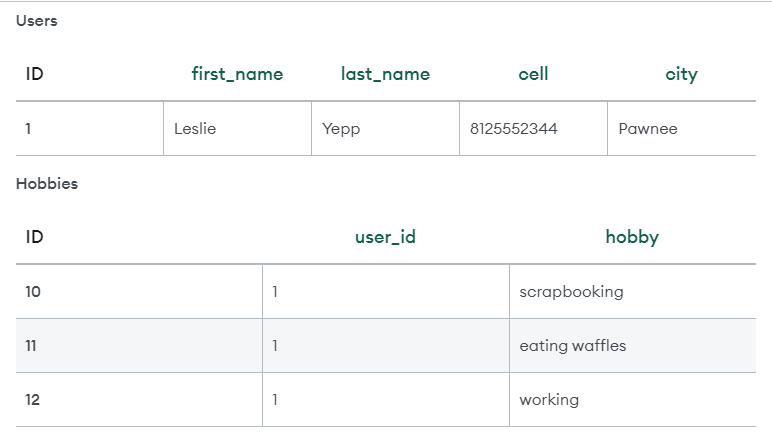
\includegraphics[width=12cm]{gambar/mongoDB1.png}
	\caption{Pemodelan RDBMS. \\ Sumber: https://www.mongodb.com/nosql-explained/}
	\label{Gambar:registrasi blueprint}
\end{figure}

\begin{figure}[H]
	\centering
	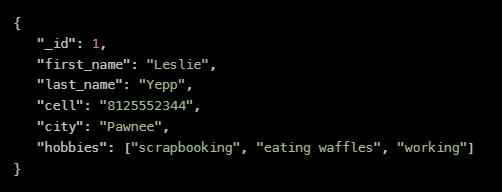
\includegraphics[width=12cm]{gambar/mongoDB2.png}
	\caption{Pemodelan NoSQL. \\ Sumber: https://www.mongodb.com/nosql-explained/}
	\label{Gambar:registrasi blueprint}
\end{figure}

Pada \textbf{Gambar 2.4} pada halaman sebelumnya, digunakan untuk menyimpan data \emph{user} dan data \emph{hobbies} dibutuhkan dua tabel terpisah dimana hal ini tidak dibutuhkan pada pemodelan NoSQL (\textbf{Gambar 2.5}) yang dapat menggabungkan dua data \emph{user} dan \emph{hobbies} pada satu dokumen serta baris yang sama. Dengan NoSQL ketika ingin memanggil dua data tersebut secara bersamaan hanya membutuhkan satu dokumen saja tanpa menggunakan \emph{joins}, yang menghasilkan \emph{queries} jauh lebih cepat dibandingkan dengan RDBMS.

\begin{enumerate}
	\item Integrasi MongoDB dan \emph{Flask}
	
	\emph{Database} MongoDB dapat diintegrasikan dengan \emph{framework flask} dengan menggunakan ekstensi yang tersedia, PyMongo adalah salah satunya. PyMongo memiliki perintah yang sama dengan perintah CLI MongoDB diantaranya membuat data, mengakses data, dan memodifikasi data. Untuk mengintegrasikan \emph{Flask} dan MongoDB diperlukan terlebih dahulu untuk menginisialisaikan projek \emph{flask} dan mengimpor ekstensi Flask-PyMongo.
	
	\begin{figure}[H]
		\centering
		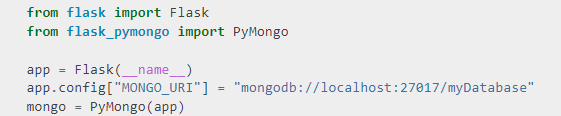
\includegraphics[width=12cm]{gambar/mongoDB3.png}
		\caption{Menambahkan Ekstensi PyMongo pada Flask. \\ Sumber: Dokumentasi PyMongo, https://flask-pymongo.readthedocs.io/en/latest/}
		\label{Gambar:registrasi blueprint}
	\end{figure}

	Inisialisasi MongoDB pada projek \emph{flask} dilakukan dengan menggunakan konstruktor PyMongo yang menerima objek app \emph{Flask} dan URI \emph{string} dari \emph{database} MongoDB. Setelah \emph{flask} dan MongoDB terintegrasi, fungsi-fungsi yang dapat kita lakukan adalah sebagai berikut:
	
	\begin{enumerate}
		\item Membuat Dokumen
		
		Metode PyMongo yang digunakan untuk menambahkan data ke dalam \emph{database} adalah db.\emph{collection}.\emph{insert\_one}() jika terdapat hanya satu data dan db.\emph{collection}.\emph{insert\_many}() jika terdapat lebih dari satu data. Untuk menambahkan dokumen ke dalam koleksi MongoDB, diperlukan untuk mendefinisikan \emph{dictionary} yang terdiri atas \emph{fields} dan \emph{values}.
		
			\begin{figure}[H]
				\centering
				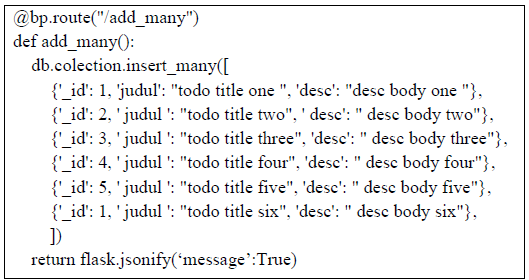
\includegraphics[width=12cm]{gambar/mongoDB4.png}
			\end{figure}
		
		Ketika mendefinisikan lebih dari satu data yang sama \emph{BulkWriteError} akan muncul, yang berarti hanya ada satu data yang terekam dan data lainnya yang sama akan hilang. Untuk mencegah hal tersebut, parameter \emph{ordered} pada fungsi \emph{insert\_many()} harus didefinisikan sebagai \emph{false} kemudian menangkap eksepsi \emph{BulkWriteError}.
		
		\item Membaca Dokumen
		
		\emph{Flask}-PyMongo memiliki beberapa metode dalam menerima data dari \emph{database}. Penerimaan semua dokumen dari koleksi menggunakan metode \emph{find()} untuk menerima semua data di \emph{database} dan \emph{find\_one()} untuk menerima satu data sesuai dengan ID yang diberikan. Metode \emph{find()} dapat menerima parameter yang digunakan sebagai \emph{filter}. Parameter \emph{filter} yang digunakan menjelaskan diksi yang mendefinisikan properti yang akan dicari.
		
		\item Memperbaharui dan Mengganti Dokumen
		
		Metode yang digunakan dalam memperbaharui data pada \emph{database} adalah \emph{update\_one()} atau \emph{replace\_one()}. Metode \emph{replace\_one()} mempunyai beberapa argumen sebagai berikut:
		
		\begin{enumerate}
			\item \emph{Filter}: berupa \emph{query} yang mendefinisikan data pada ID yang akan diganti,
			
			\item \emph{Replacement}: berupa data yang akan menggantikan data yang dihapus.
			
			\item \emph{Upsert}: adalah opsi \emph{boolean} yang jika dijadikan sebagai \emph{true} dapat membuat dokumen baru jika tidak terdapat target dokumen yang dimaksud.
			
		\end{enumerate}
	
	\item Menghapus Dokumen
	
	PyMongo menyediakan dua metode untuk menghapus satu atau lebih koleksi \emph{database} yaitu, \emph{delete\_one()} untuk menghapus satu koleksi dan \emph{delete\_many()} untuk menghapus beberapa koleksi.
	
	\begin{figure}[H]
		\centering
		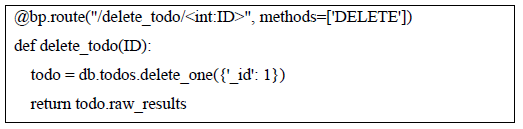
\includegraphics[width=12cm]{gambar/mongoDB5.png}
	\end{figure}

	Contoh kode di atas ketika menjalankan \emph{request} seperti http://\emph{localhost}:5000/\emph{delete}\_todo/5 PyMongo akan mencari entri berdasarkan ID yang diberikan dan menghapusnya.
	
	\item Menyimpan dan Menerima \emph{Files}
	
	MongoDB mengizinkan pengembang untuk menyimpan data biner ke dalam \emph{database} menggunakan spesifikasi GridFS. Ekstensi Flask-PyMongo menyediakan metode \emph{save\_file()} untuk menyimpan \emph{file} ke GridFS dan metode \emph{send\_file()} untuk menerima \emph{file} dari GridFS
	
	\begin{figure}[H]
		\centering
		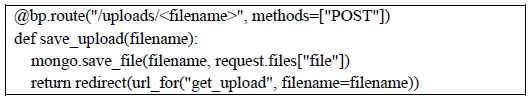
\includegraphics[width=12cm]{gambar/mongoDB6.png}
	\end{figure}
	
	Kode di atas, dibuat \emph{form} untuk menangani unggahan file dan mengembalikan nama \emph{file} yang telah terunggah.
		
	\end{enumerate}
	
\end{enumerate}

\section{Scrum}

\emph{Scrum} merupakan salah satu struktur kerja yang digunakan untuk mengembangkan produk. \emph{Scrum} diumumkan pertama kali oleh Ken Schwaber pada tahun 1995 pada konferensi Austin, namun fondasi metode \emph{scrum} sudah ada sejak tahun 1980 \citep{Oziera2016The}. \emph{Scrum} dibuat berdasarkan empirisme yang dicapai dengan beberapa kualitas. Hasil survei dari literatur, kualitas yang membangun empirisme \emph{scrum} adalah kejelasan dari setiap proses, inspeksi untuk mendeteksi masalah dan adaptasi terhadap perubahan

Setiap produk dihantarkan dengan cara yang fleksibel dan iteratif dalam kerangka kerja \emph{scrum} dimana setiap akhir \emph{sprint} terdapat produk nyata yang dapat dihantarkan. \emph{Requirement} yang dibutuhkan dalam suatu proyek berupa \emph{product backlog} yang diperbaharui secara berkala.

\emph{Scrum} mempunyai tiga elemen, di antaranya:

\begin{enumerate}
	\item \emph{Roles}
	
	\emph{Role} dalam \emph{scrum} terbagi menjadi empat \emph{role} utama, yaitu:
	
	\begin{enumerate}
		\item Tim \emph{Scrum}
		
		Tim \emph{scrum} merupakan kelompok kecil yang terdiri dari satu \emph{scrum master}, satu \emph{product owner}, dan pengembang. Pada tim \emph{scrum} tidak terdapat tim kecil ataupun hierarki. Seluruh anggota tim memiliki kemampuan penting untuk memberikan nilai ke dalam setiap \emph{sprint} dan fokus dengan satu tujuan pada satu waktu, \emph{product goal}.
		
		Tim \emph{scrum} bertanggung jawab dalam setiap aktivitas produk seperti kolaborasi dengan \emph{stakeholder}, \emph{maintenance}, verifikasi, \emph{research}, \emph{operation}, \emph{experimentation} dan pengembangan. Tim \emph{scrum} menghantarkan produk secara \emph{iterative} menggunakan \emph{sprint}, oleh karena itu tim \emph{scrum} juga bertanggung jawab untuk menciptakan nilai pada setiap \emph{sprint}-nya.
		
		\break
		
		\item \emph{Scrum Master}
		
		\emph{Scrum master} memiliki tanggung jawab dalam merealisasikan \emph{scrum} yang terdefinisi pada panduan \emph{scrum}. Setiap anggota tim dibantu \emph{scrum master} untuk mengerti bagaimana teori dan praktik kerangka kerja pada metode \emph{scrum}. Selain itu, menjaga efektivitas dari tim \emph{scrum} juga menjadi tanggung jawab \emph{scrum master}.
		
		\item \emph{Product Owner}
		
		\emph{Product owner} memiliki tanggung jawab untuk meningkatkan nilai komersial produk yang dihasilkan oleh \emph{development team} dan mengelola \emph{product backlog} agar lebih maksimal. Hanya \emph{product owner} yang memiliki tanggung jawab untuk mengelola \emph{product backlog}. Adapun pengelolaan \emph{product backlog}:
		
		\begin{enumerate}
			\item Penyampaian isi \emph{product backlog}.
			\item Memastikan \emph{development team} memahami \emph{product backlog}.
			\item Memastikan isi daripada \emph{product backlog} transparan dan jelas bagi seluruh anggota tim.
			\item Mengurutkan item pada \emph{product backlog} untuk mencapai tujuan secara optimal.
			
		\end{enumerate}
	
		\item \emph{Development Team}
		
		\emph{Development team} atau tim pengembang adalah profesional yang mengeksekusi isi yang tercantum di dalam \emph{product backlog}. Tim Pengembang berkomitmen untuk membuat semua aspek \emph{increment} yang dapat berfungsi pada setiap \emph{sprint}. Namun, tim Pengembang juga selalu bertanggung jawab untuk:
		
		\begin{enumerate}
			\item Membuat rancangan \emph{sprint} atau dikenal dengan \emph{sprint backlog}.
			\item Membuat definisi penyelesaian sebuah \emph{task}.
			\item Mengadaptasikan semua \emph{plan} setiap hari sampai \emph{sprint goal}.
			\item Mengurutkan \emph{item} pada \emph{product backlog} untuk mencapai tujuan secara optimal.
			
		\end{enumerate}
		
	\end{enumerate}
	
	\item \emph{Artifacts}
	
	Artefak \emph{scrum} dirancang untuk memaksimalkan transparansi informasi utama dan kesempatan untuk menginspeksi dan mengadaptasi.
	
	\begin{enumerate}
		\item \emph{Product Backlog}
		
		\emph{Product backlog} atau umumnya disebut dengan \emph{user stories} merupakan kumpulan fitur-fitur yang terdapat pada suatu produk . \emph{User stories} dapat ditambahkan, dimodifikasi, atau dihilangkan dari \emph{product backlog} selama proyek berjalan.
		
		\item \emph{Sprint Backlog}
		
		\emph{Sprint backlog} adalah beberapa \emph{user stories} yang diambil dari \emph{product backlog} untuk dijalankan pada satu \emph{sprint}. \emph{Sprint backlog} mencakup seluruh kegiatan kerja yang diperlukan untuk mencapai \emph{sprint goal}.
		
		Pada satu \emph{sprint} terdapat \emph{increment} yang merupakan manifestasi dari \emph{user stories} yang diselesaikan dan total \emph{increment} dari seluruh \emph{sprint} sebelumnya.
		
	\end{enumerate}
	
	\item Events
	
	\emph{Event} merupakah wadah dari semua \emph{event} yang terdapat pada \emph{scrum}. \emph{Event} dibuat sebagai perwujudan salah satu dari tiga pilar \emph{scrum}. Seluruh \emph{event} berjalan secara bersamaan untuk mengurangi kompleksitas.
	
		\begin{enumerate}
		\item \emph{Sprint}
		
		\emph{Sprint} adalah komponen utama kerangka kerja \emph{scrum}, dimana sebuah ide menjadi sebuah nilai. Lama durasi \emph{sprint} bersifat tetap yaitu satu hingga empat minggu untuk menjaga konsistensi.
		
		\emph{Sprint} berfokus untuk menghantarkan beberapa \emph{user stories} pada \emph{product backlog}. Setiap satu \emph{sprint} memiliki beberapa kegiatan diantaranya \emph{sprint planning}, \emph{sprint review} dan \emph{sprint retrospective}.
		
		\item \emph{Sprint Planning}
		
		\emph{Sprint backlog} adalah beberapa \emph{user stories} yang diambil dari \emph{product backlog} untuk dijalankan pada satu \emph{sprint}. \emph{sprint backlog} mencakup semua kegiatan kerja yang dibutuhkan untuk mencapai \emph{sprint goal}.
		
		Sebelum memulai \emph{sprint}, perencanaan apa yang akan dilaksanakan pada saat \emph{sprint} dilakukan pada saat \emph{sprint planning} oleh seluruh anggota tim \emph{scrum}. Waktu untuk melaksanakan \emph{sprint planning} terbatas dengan lama durasi hingga delapan jam. Fungsi dari \emph{sprint planning} adalah memutuskan apa yang dapat dimasukkan ke dalam \emph{increment} dari \emph{sprint} dan bagaimana penyelesaian yang dibutuhkan untuk menghantarkan \emph{increment}.
		
		\item \emph{Daily Scrum}
		
		\emph{Daily scrum} adalah kegiatan 15 menit bagi para pengembang untuk memeriksa perkembangan menuju \emph{sprint goal} dan menyesuaikan pekerjaan yang akan dikerjakan selama 24 jam ke depan. Pada kegiatan \emph{daily scrum}, hal apa saja yang akan dikerjakan hari ini, apa yang telah dikerjakan kemarin dan hambatan yang telah dialami dalam mencapai \emph{sprint goal} akan didiskusikan oleh tim pengembang.
		
		\break
		\item \emph{Sprint Review}
		
		Tahap ini dilaksanakan pada akhir \emph{sprint}, tujuannya untuk mengawasi apa yang telah diselesaikan di \emph{sprint}. Menurut hasil tinjauan serta perubahan \emph{product backlog}, tim \emph{scrum} menentukan kembali pekerjaan selanjutnya yang dapat mengoptimalkan produk.
		
		\emph{Sprint review} bersifat informal dan diselenggarakan dengan lama durasi empat jam untuk sprint dalam waktu satu bulan. Semakin singkat durasi \emph{sprint}, maka semakin singkat juga durasi \emph{sprint review}.
		
	\end{enumerate}
	
\end{enumerate}

\begin{comment}
\section{Studi Banding Sistem Informasi Rumah Sakit}

Dalam melakukan studi banding, peneliti menggunakan 3 jurnal yang didapat dari internet. Jurnal pertama peneliti ambil dari penelitian yang dilakukan oleh Ardiansyah dengan judul "Analisis dan Perancangan Sistem Informasi Manajemen Rumah Sakit Berbasis \emph{Website} Pada Rumah Sakit Umum Kambang Kota Jambi". \citep{Ardiansyah2021analisis:10}. Jurnal kedua peneliti ambil dari jurnal yang berjudul "Sistem Informasi Rekam Medis Pada Rumah Sakit Umum Daerah (RSUD) Pacitan Berbasis \emph{Web Base}" oleh Gunawan Susanto. \citep{Gunawan2011sistem:11}. Dan Jurnal Ketiga peneliti ambil dari penelitian yang dilakukan oleh Inah Carminah dengan judul "Aplikasi Monitoring Perawatan Luka Diabetes Melitus Berbasis \emph{Website}". \cite{Carminah2021aplikasi:12}.

\subsection{Studi Banding Berdasarkan Fitur}
Berikut diagram \emph{use case} dari ketiga jurnal yang telah peneliti sebutkan di atas.

\begin{enumerate}
	\item Diagram \emph{use case} pada jurnal pertama
	
	Diagram \emph{use case} ada pada halaman berikutnya pada \textbf{Gambar 2.1}
	\begin{figure}[H]
		\centering
		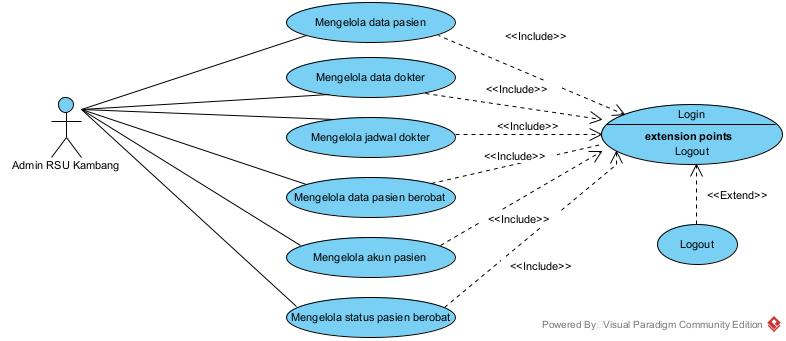
\includegraphics[width=12cm]{gambar/jurnal1_use_case_admin.jpg}
		\caption{Diagram \emph{use case} admin jurnal pertama \\ Sumber: \citep{Ardiansyah2021analisis:10}} 
		\label{Gambar:usecaseadminjurnalpertama}
	\end{figure}
	
	\begin{figure}[H]
		\centering
		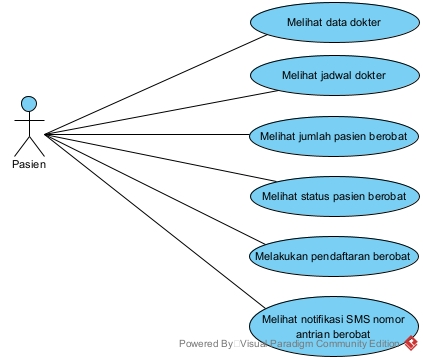
\includegraphics[width=12cm]{gambar/jurnal1_use_case_pasien.jpg}
		\caption{Diagram \emph{use case} pasien jurnal pertama \\ Sumber: \citep{Ardiansyah2021analisis:10}}
		\label{Gambar:usecasepasienjurnalpertama}
	\end{figure}
	
	\item \emph{Data flow diagram}(DFD) pada jurnal kedua.
	
	Pada jurnal kedua tidak ditemukan \emph{use case} diagram dan hanya tersedia \emph{data flow diagram}. Berikut \emph{data flow diagram} pada jurnal kedua.
	
	\begin{figure}[H]
		\centering
		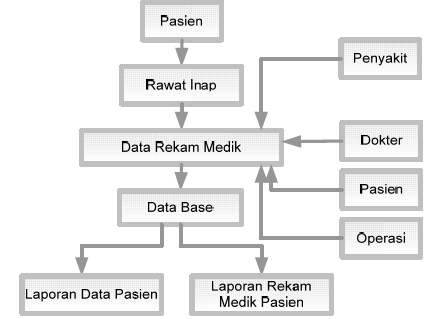
\includegraphics[width=8cm]{gambar/data_flow_diagram_jurnal2.png}
		\caption{Diagram \emph{data flow diagram} jurnal kedua \\ Sumber: \citep{Gunawan2011sistem:11}}
		\label{Gambar:dataflowdiagramjurnalkedua}
	\end{figure}
	
	\item Diagram \emph{use case} pada jurnal ketiga
	
	\begin{figure}[H]
		\centering
		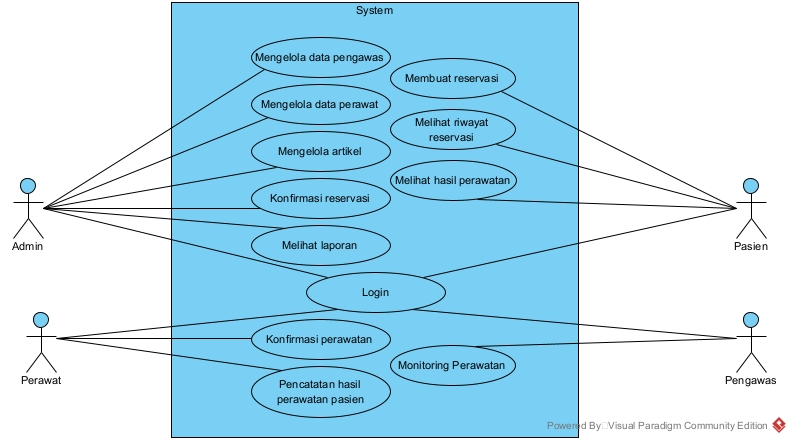
\includegraphics[width=12cm]{gambar/diagram_use_case_jurnal3.jpg}
		\caption{Diagram \emph{use case} jurnal ketiga \\ Sumber: \citep{Carminah2021aplikasi:12}}
		\label{Gambar:usecasejurnalketiga}
	\end{figure}
	
\end{enumerate}

\subsection{Studi Banding Berdasarkan UI/UX}

\begin{enumerate}
	\item UI/UX pada jurnal pertama
	
	Berikut di bawah ini merupakan UI/UX yang ditampilkan didalam jurnal pertama: 
	
	\textbf{Gambar 2.5} menampilkan rancangan halaman utama registrasi \emph{online} RSU Kambang yang berisi sosial media, dan alamat beserta tombol menu.
	
	\begin{figure}[H]
		\centering
		
\includegraphics[width=12cm]{gambar/halaman_utama_registrasi_online.png}
		\caption{Rancangan halaman registrasi \emph{online} \\ Sumber: \citep{Ardiansyah2021analisis:10}}
		\label{Gambar:halamanutamaregistrasionline}
	\end{figure}
	
	\begin{figure}[H]
		\centering
		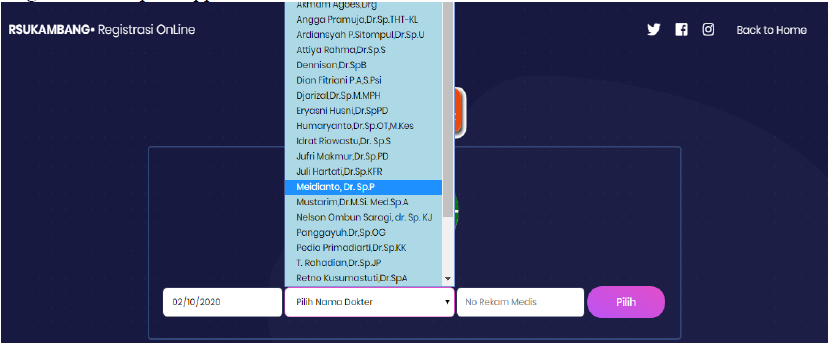
\includegraphics[width=12cm]{gambar/halaman_pilih_appointment.png}
		\caption{Rancangan Halaman pilih \emph{appointment} \\ Sumber: \citep{Ardiansyah2021analisis:10}}
		\label{Gambar:halamanpilihappointment}
	\end{figure}
	
	\textbf{Gambar 2.6} menampilkan rancangan halaman \emph{appointment} RSU Kambang yang berisi \emph{field} tanggal \emph{appointment}, \emph{field} nama dokter yang dituju, \emph{field} nomor rekam medis, sosial media, tombol pilih dan tombol \emph{back to home}.
	
	\textbf{Gambar 2.7} pada halaman selanjutnya menampilkan rancangan daftar pasien yang sudah mendaftar berobat RSU Kambang yang berisi tanggal, nama dokter, sosial media, tombol \emph{back to home}. Lalu ada tabel berupa nomor, nomor rekam medis, nama pasien, nomor antrian, dan status beserta tombol daftar shift pagi dan shift siang.
	
	\begin{figure}[H]
		\centering
		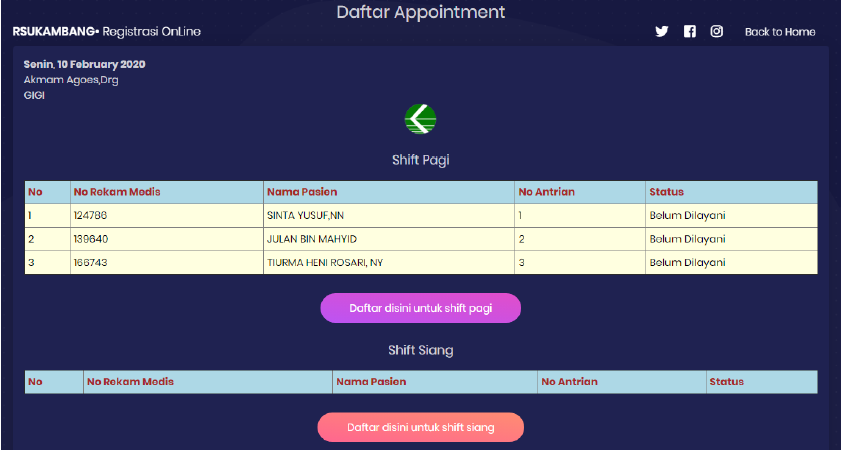
\includegraphics[width=12cm]{gambar/halaman_tampil_daftar_pasien_mendaftar.png}
		\caption{Rancangan halaman daftar pasien yang sudah mendaftar berobat \\ Sumber: \citep{Ardiansyah2021analisis:10}}
		\label{Gambar:halamandaftarpasienyangsudahmendaftar}
	\end{figure}
	
	\begin{figure}[H]
		\centering
		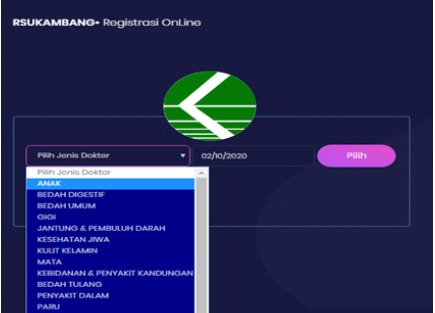
\includegraphics[width=10cm]{gambar/halaman_jadwal_dokter.png}
		\caption{Rancangan halaman jadwal dokter \\ Sumber: \citep{Ardiansyah2021analisis:10}}
		\label{Gambar:halamanjadwaldokter}
	\end{figure}
	
	\textbf{Gambar 2.8} pada halaman sebelumnya menampilkan rancangan halaman jadwal dokter yang berisi \emph{field} pilih jenis dokter dan \emph{field} tanggal beserta tombol pilih.
	
	\textbf{Gambar 2.9} menampilkan rancangan halaman \emph{input} registrasi berobat yang berisi \emph{field} nama dokter, \emph{field} nomor rekam medis, \emph{field} nama pasien, \emph{field} pilihan pendaftaran, \emph{field} nomor \emph{handphone}, \emph{field} tanggal lahir, \emph{field} jam registrasi berobat beserta \emph{field} tanggal registrasi berobat.
	
	\begin{figure}[H]
		\centering
		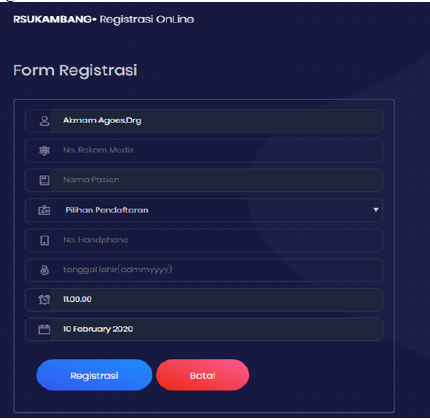
\includegraphics[width=10cm]{gambar/halaman_input_registrasi.png}
		\caption{Rancangan halaman \emph{input} registrasi berobat \\ Sumber: \citep{Ardiansyah2021analisis:10}}
		\label{Gambar:halamaninputregistrasiobat}
	\end{figure}
	
	\textbf{Gambar 2.10} pada halaman selanjutnya menampilkan rancangan halaman utama admin yang berisi ucapan selamat datang, foto RSU Kambang Jambi, beserta tombol pengaturan.
	
	\begin{figure}[H]
		\centering
		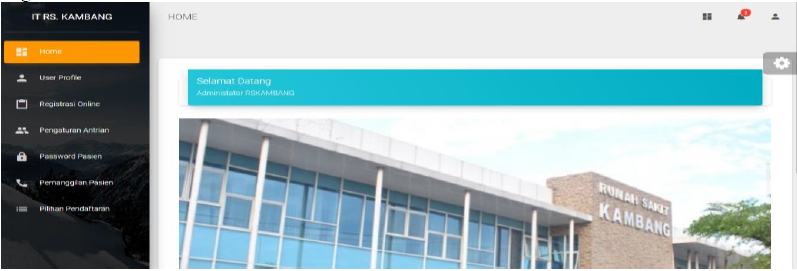
\includegraphics[width=12cm]{gambar/halaman_utama_admin.png}
		\caption{Rancangan halaman utama admin \\ Sumber: \citep{Ardiansyah2021analisis:10}}
		\label{Gambar:halamanutamaadmin}
	\end{figure}
	
	\textbf{Gambar 2.11} menampilkan rancangan halaman \emph{user profile} yang berisi tombol pengaturan, dan tabel Data Login Admin yang berisi \emph{username}, nama, Jabatan, No. HP, Email, Status, dan Opsi.
	
	\begin{figure}[H]
		\centering
		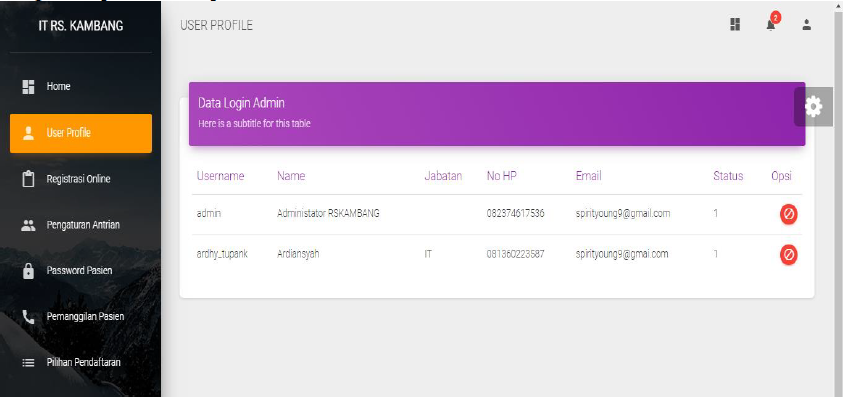
\includegraphics[width=12cm]{gambar/halaman_tampil_data_user_profile.png}
		\caption{Rancangan halaman \emph{user profile} \\ Sumber: \citep{Ardiansyah2021analisis:10}}
		\label{Gambar:halamanuserprofile}
	\end{figure}
	
	\textbf{Gambar 2.12} pada halaman selanjutnya menampilkan rancangan halaman \emph{user} yang melakukan registrasi \emph{online} yang berisi \emph{field} tanggal, tombol pilih, tombol pengaturan, tabel data registrasi pasien yang berisi Nama Daftar, No. RM, No. HP, Tanggal Registrasi, Tanggal Berobat, Status, Nama Dokter, dan Aksi.
	
	\begin{figure}[H]
		\centering
		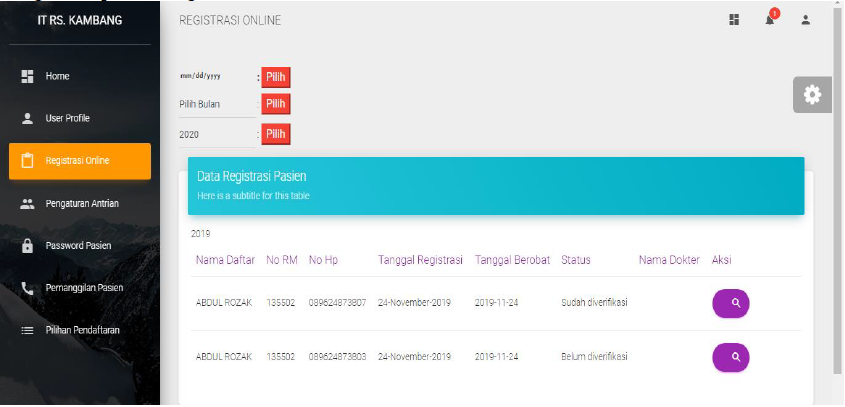
\includegraphics[width=12cm]{gambar/halaman_tampil_data_registrasi_online.png}
		\caption{Rancangan halaman \emph{list user} melakukan registrasi \emph{online} \\ Sumber: \citep{Ardiansyah2021analisis:10}}
		\label{Gambar:halamanusermelakukanregistrasi}
	\end{figure}
	
	\textbf{Gambar 2.13} menampilkan rancangan halaman detail data \emph{user} yang melakukan registrasi \emph{online} yang berisi tabel data registrasi antrian berupa No. RM, Nama, Tanggal Lahir, No. Telephone, Tanggal Registrasi, No. HP, Status, dan No. Antrian. Terdapat tabel informasi dokter yang dituju berupa Nama Dokter, Status Dokter, Jam Dokter, Tanggal Berobat, dan Poliklinik. Tabel \emph{cancel} berupa status antrian dan keterangan. Dan ada tombol pengaturan.
	
	\begin{figure}[H]
		\centering
		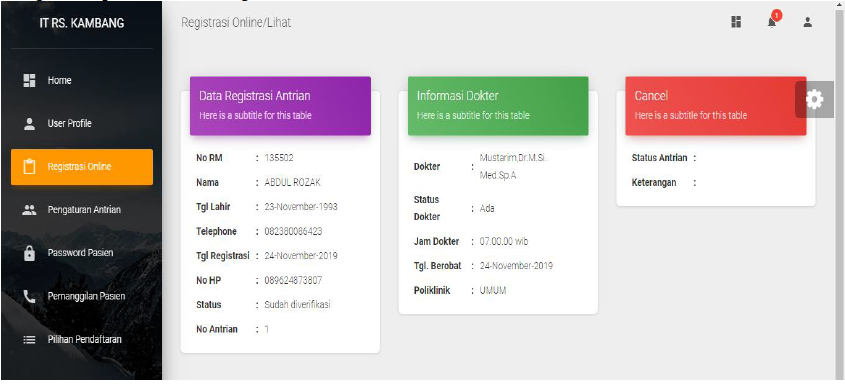
\includegraphics[width=12cm]{gambar/halaman_tampil_detail_data_registrasi_online.png}
		\caption{Rancangan halaman detail data \emph{user} melakukan registrasi \emph{online} \\ Sumber: \citep{Ardiansyah2021analisis:10}}
		\label{Gambar:halamandetaildatausermelakukanregistrasionline}
	\end{figure}
	
	\textbf{Gambar 2.14} pada halaman selanjutnya menampilkan rancangan halaman tampil daftar alasan \emph{cancel} registrasi yang berisi tabel alasan \emph{cancel} registrasi berupa Nomor, alasan, tombol tambah data, edit dan hapus.
	
	\begin{figure}[H]
		\centering
		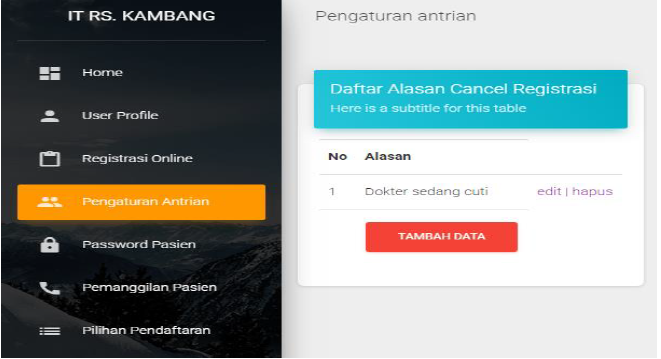
\includegraphics[width=10cm]{gambar/halaman_tampil_daftar_alasan_cancel_registrasi.png}
		\caption{Rancangan halaman daftar alasan \emph{cancel} registrasi \\ Sumber: \citep{Ardiansyah2021analisis:10}}
		\label{Gambar:halamandaftaralasancancelregistrasi}
	\end{figure}
	
	Berikut merupakan tampilan UI/UX live pada website  \emph{live} RSU Kambang Jambi pada \url{https://rsukambang.com/}
	
	\begin{figure}[H]
		\centering
		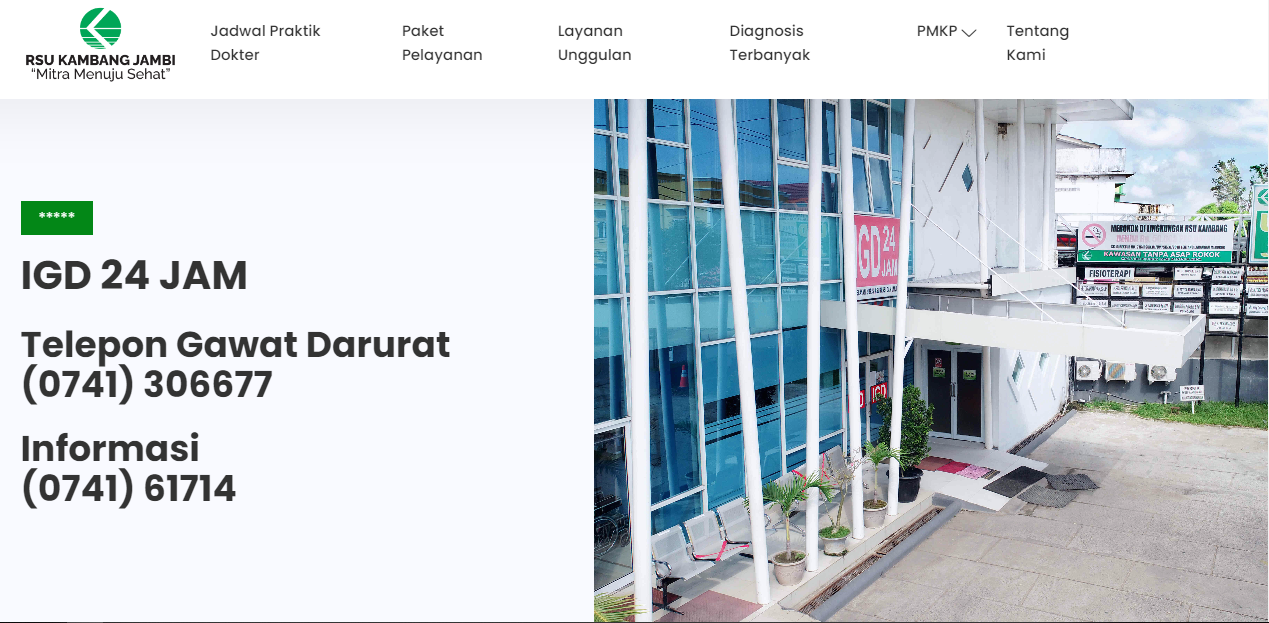
\includegraphics[width=12cm]{gambar/halaman_utama_rsu_kambang_jambi_live.png}
		\caption{halaman utama RSU Kambang \emph{live} \\ Sumber: \url{https://rsukambang.com/}}
		\label{Gambar:halamanutamarsukambanglive}
	\end{figure}
	
	\textbf{Gambar 2.15} menampilkan halaman utama RSU Kambang \emph{live} yang berisi informasi nomor \emph{telephone}, visi, misi, info pelayanan, daftar berobat via whatsapp. (\textbf{Gambar 2.16}) pada halaman berikutnya berisi info asuransi yang diterima, dan lokasi RS.
	
	\begin{figure}[H]
		\centering
		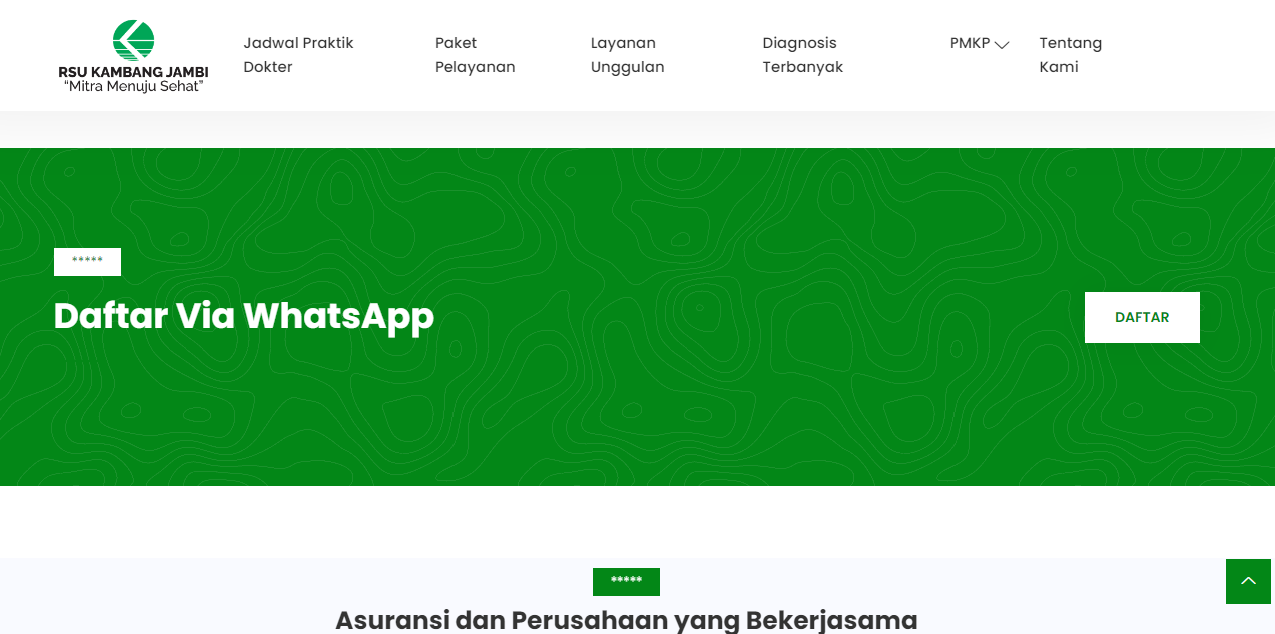
\includegraphics[width=12cm]{gambar/halaman_utama_lanjutan_daftar_berobat_live.png}
		\caption{halaman utama RSU Kambang \emph{live} lanjutan \\ Sumber: \url{https://rsukambang.com/}}
		\label{Gambar:halamanutamarsukambanglivelanjutan}
	\end{figure}
	
	\textbf{Gambar 2.17} menampilkan halaman jadwal praktik dokter \emph{live} yang berisi \emph{flyer} jadwal praktik dokter.
	
	\begin{figure}[H]
		\centering
		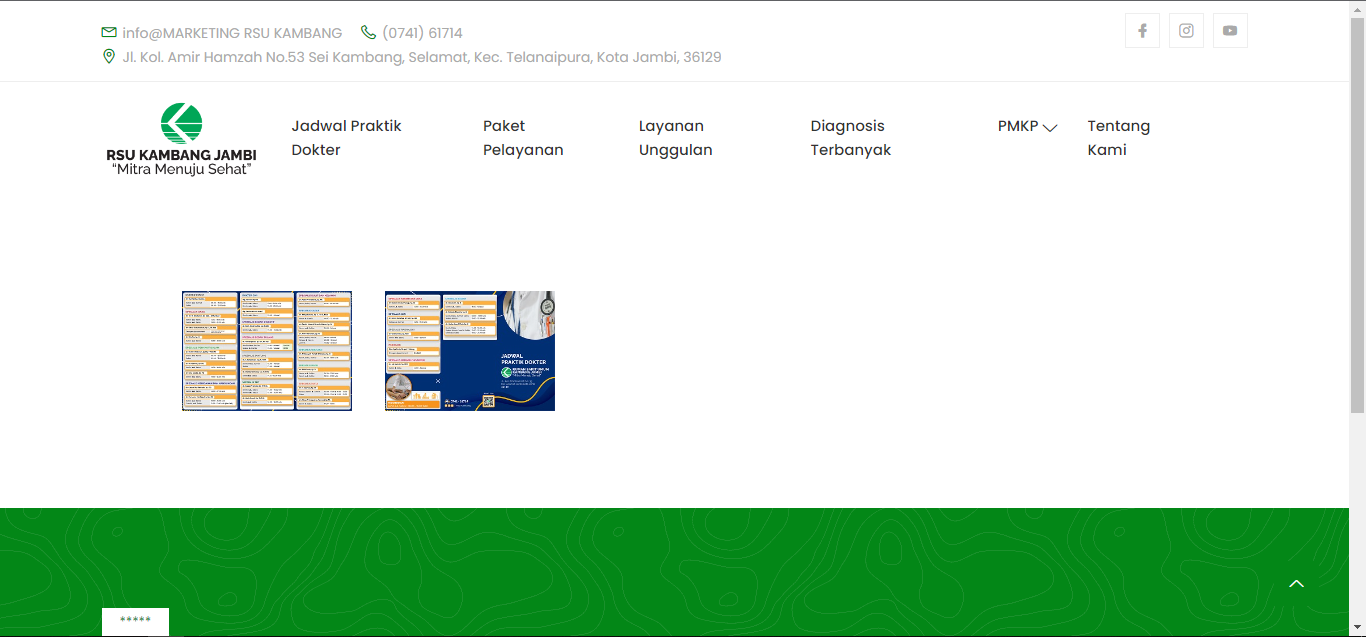
\includegraphics[width=12cm]{gambar/halaman_jadwal_praktik_dokter_rsu_kambang_live.png}
		\caption{halaman jadwal praktik dokter \emph{live} \\ Sumber: \url{https://rsukambang.com/}}
		\label{Gambar:halamanjadwalpraktikdokterlive}
	\end{figure}
	
	\textbf{Gambar 2.18} pada halaman selanjutnya menampilkan halaman paket pelayanan \emph{live} yang berisi flyer paket pelayanan beserta harganya.
	
	\begin{figure}[H]
		\centering
		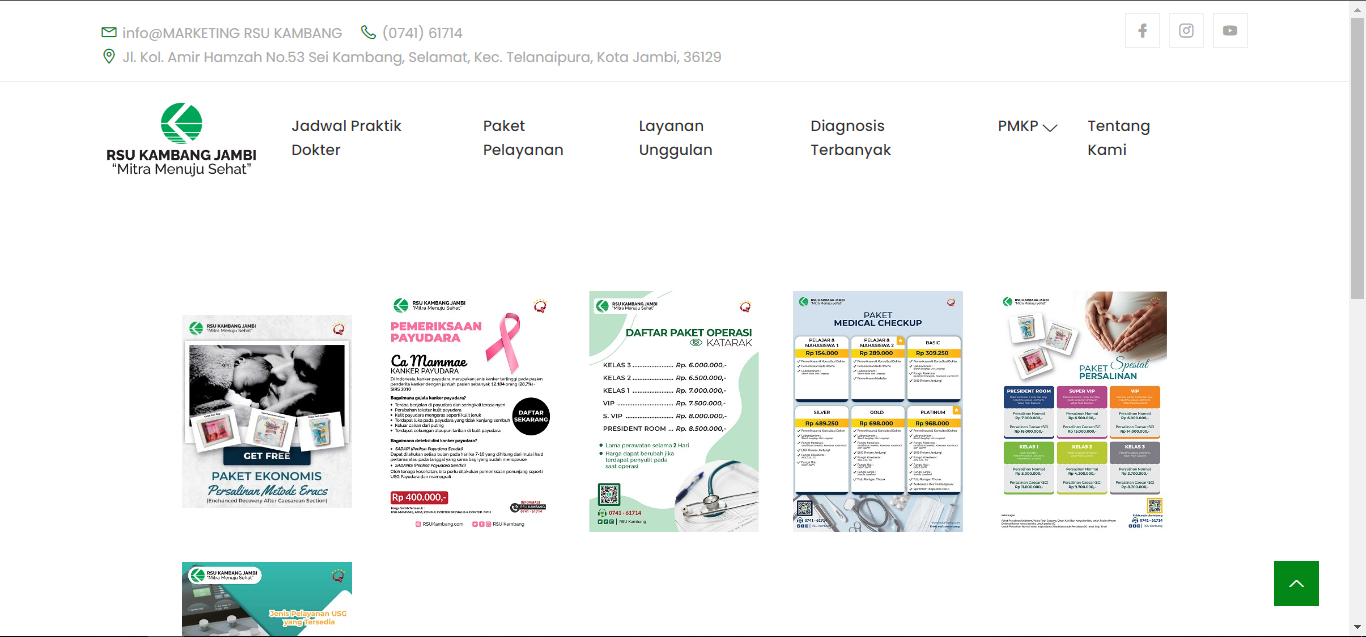
\includegraphics[width=12cm]{gambar/halaman_paket_pelayanan_live.png}
		\caption{halaman paket pelayanan \emph{live} \\ Sumber: \url{https://rsukambang.com/}}
		\label{Gambar:halamanpaketpelayananlive}
	\end{figure}
	
	
	\textbf{Gambar 2.19} menampilkan halaman layanan unggulan \emph{live} yang berisi daftar pelayanan dan penunjang medis beserta daftar sarana dan prasarana yang ada di RSU Kambang.
	
	\begin{figure}[H]
		\centering
		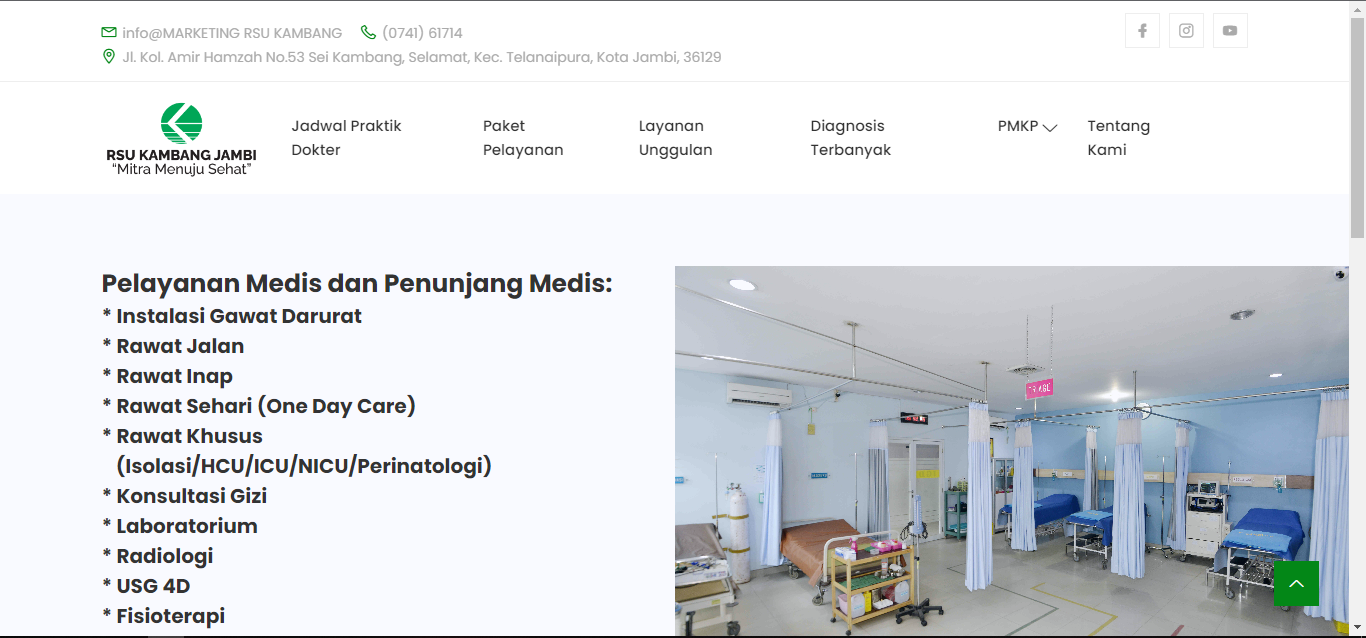
\includegraphics[width=12cm]{gambar/halaman_layanan_unggulan_live.png}
		\caption{halaman layanan unggulan \emph{live} \\ Sumber: \url{https://rsukambang.com/}}
		\label{Gambar:halamanlayananunggulanlive}
	\end{figure}
	
	\textbf{Gambar 2.20} pada halaman berikutnya menampilkan halaman diagnosis terbanyak \emph{live} yang berisis tabel daftar 10 Besar Penyakit Rawat Jalan Tahun 2022 dan tabel daftar 10 Besar Penyakit Rawat Inap Tahun 2022.
	
	\begin{figure}[H]
		\centering
		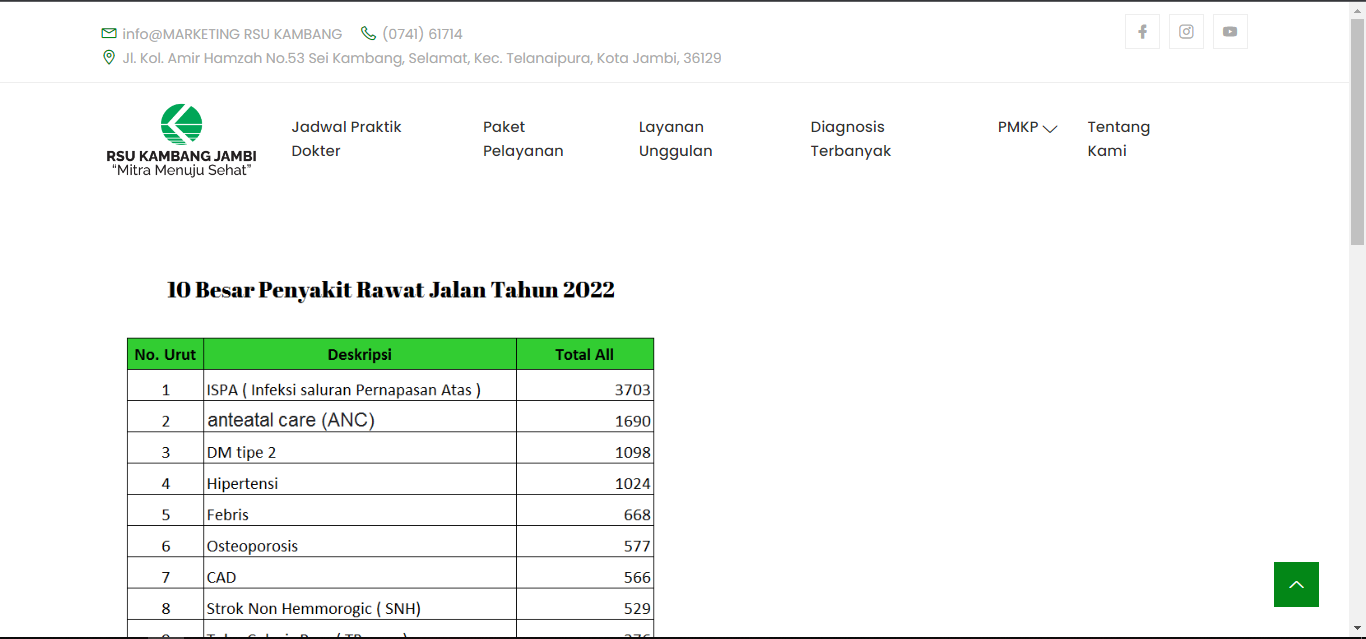
\includegraphics[width=12cm]{gambar/halaman_diagnosis_terbanyak_live.png}
		\caption{halaman diagnosis terbanyak \emph{live} \\ Sumber: \url{https://rsukambang.com/}}
		\label{Gambar:halamandiagnosisterbanyaklive}
	\end{figure}
	
	\textbf{Gambar 2.21} menampilkan halaman PKMP \emph{live} yang berisi 13 indikator nasional mutu dalam bentuk grafik.
	
	\begin{figure}[H]
		\centering
		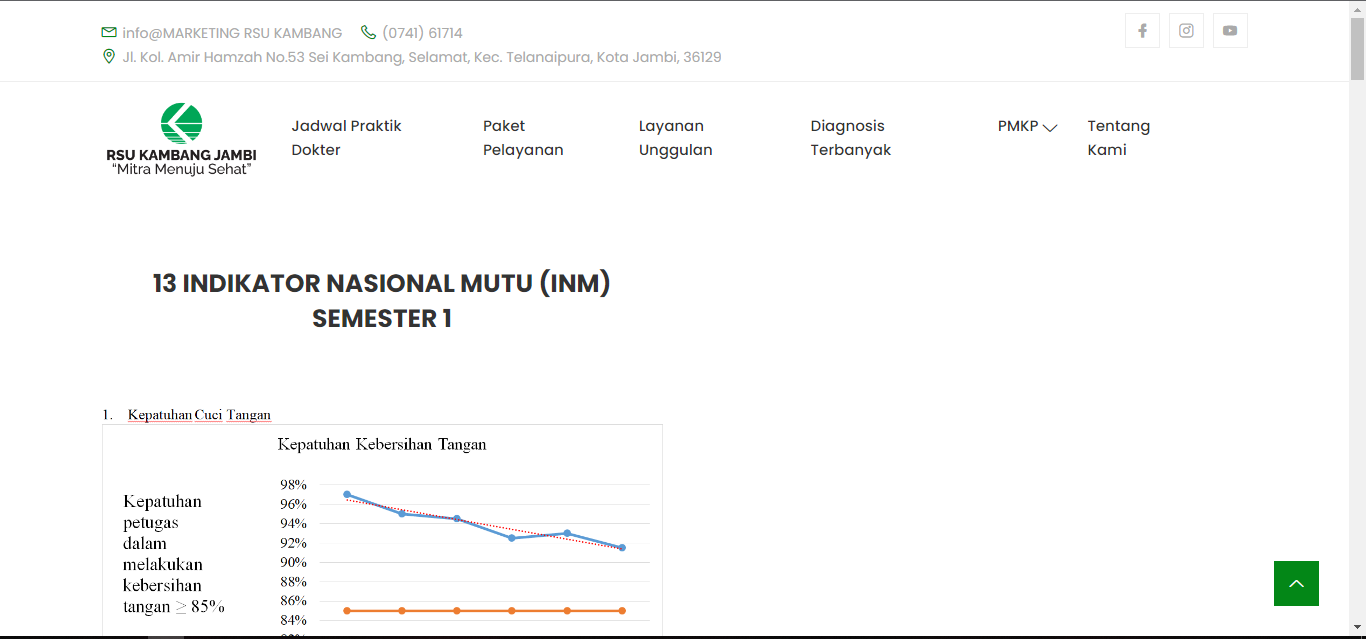
\includegraphics[width=12cm]{gambar/halaman_pkmp_live.png}
		\caption{halaman pkmp \emph{live} \\ Sumber: \url{https://rsukambang.com/}}
		\label{Gambar:halamanpkmplive}
	\end{figure}
	
	\textbf{Gambar 2.22} pada halaman selanjutnya menampilkan halaman tentang kami \emph{live} yang berisi profil, visi, dan misi RSU Kambang Jambi.
	
	\begin{figure}[H]
		\centering
		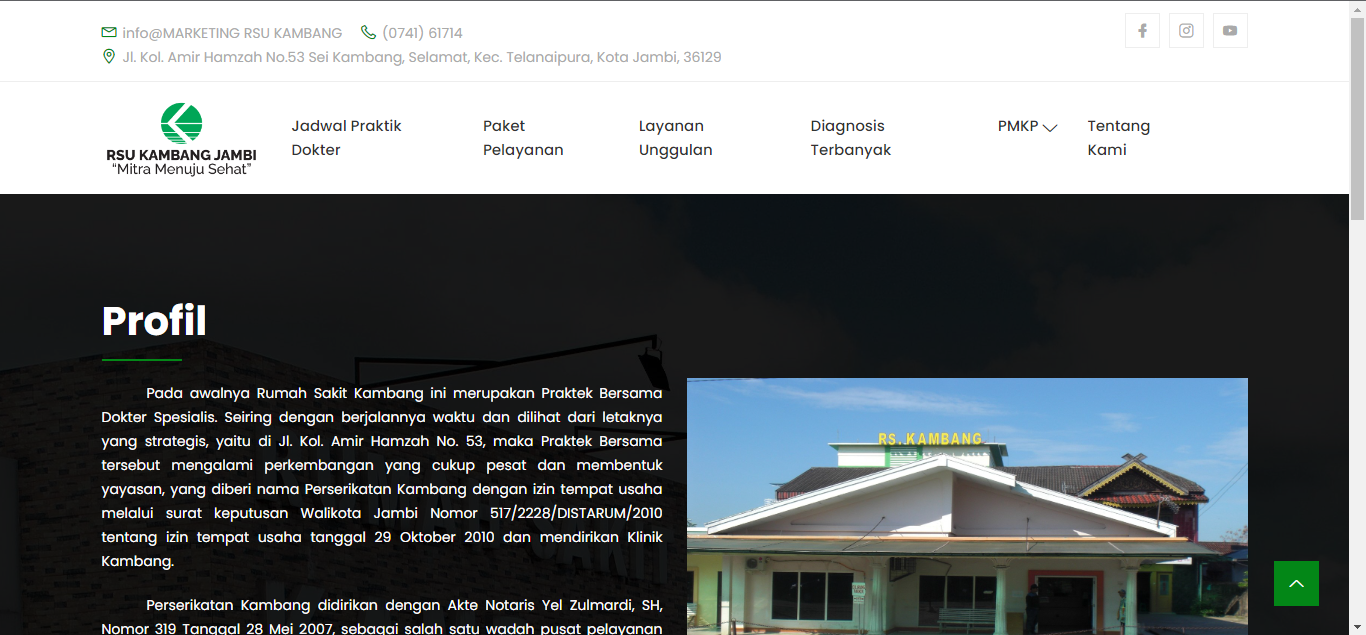
\includegraphics[width=12cm]{gambar/halaman_tentang_kami_live.png}
		\caption{halaman tentang kami \emph{live} \\ Sumber: \url{https://rsukambang.com/}}
		\label{Gambar:halamantentangkamilive}
	\end{figure}
	
	\item UI/UX pada jurnal kedua
	
	Berikut di bawah ini merupakan UI/UX yang ditampilkan didalam jurnal kedua:
	
	\begin{figure}[H]
		\centering
		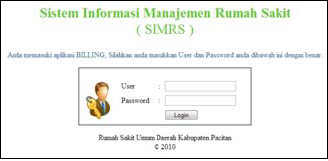
\includegraphics[width=12cm]{gambar/halaman_login.png}
		\caption{Rancangan halaman \emph{login} Sistem Informasi Manajemen Rumah Sakit \\ Sumber: \citep{Gunawan2011sistem:11}}
		\label{Gambar:halamanloginsisteminformasimanajemenrumahsakit}
	\end{figure}
	
	\textbf{Gambar 2.23} menampilkan rancangan halaman \emph{login} Sistem Informasi Manajemen Rumah Sakit yang berisi \emph{field} user dan \emph{field password} beserta tombol login.
	
	\begin{figure}[H]
		\centering
		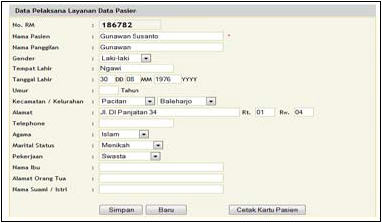
\includegraphics[width=12cm]{gambar/halaman_petugas_mendaftarkan_pasien.png}
		\caption{Rancangan halaman daftar pasien \\ Sumber: \citep{Gunawan2011sistem:11}}
		\label{Gambar:halamandaftarpasien}
	\end{figure}
	
	\textbf{Gambar 2.24} menampilkan rancangan halaman daftar pasien yang berisi \emph{field} No. RM, \emph{field} nama pasien, \emph{field} nama panggilan, \emph{field} gender, \emph{field} tempat lahir, \emph{field} tanggal lahir, \emph{field} umur, \emph{field} kecamatan/kelurahan, \emph{field} alamat/rt/rw, \emph{field telephone}, \emph{field} agama, \emph{field} marital status, \emph{field} pekerjaan, \emph{field} nama ibu, \emph{field} alamat orang tua, \emph{field} nama suami/istri,  beserta tombol simpan, baru, dan cetak kartu pasien.
	
	\begin{figure}[H]
		\centering
		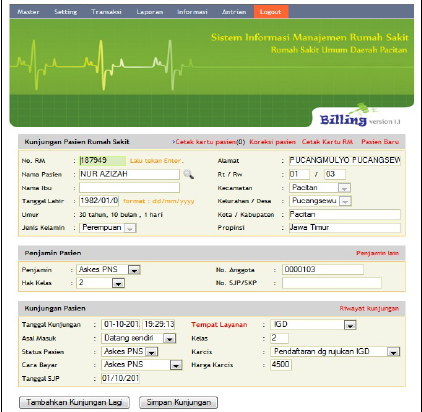
\includegraphics[width=8cm]{gambar/halaman_petugas_mengunjungkan_pasien_ke_poli.png}
		\caption{Rancangan halaman petugas mengunjungkan pasien ke poliklinik. \\ Sumber: \citep{Gunawan2011sistem:11}}
		\label{Gambar:halamanpetugasmengunjungkanpasienkepoliklinik}
	\end{figure}
	
	\textbf{Gambar 2.25} menampilkan rancangan halaman petugas mengunjungkan pasien ke poliklinik yang berisi tabel kunjungan pasien rumah sakit berisi \emph{field} No. RM, \emph{field} nama pasien, \emph{field} nama ibu, \emph{field} tanggal lahir, \emph{field} umur, \emph{field} jenis kelamin, \emph{field} alamat, \emph{field} rt/rw, \emph{field} kecamatan, \emph{field} kelurahan/desa, \emph{field} kota/kabupaten, dan \emph{field} provinsi. Lalu ada tabel penjamin pasien berisi \emph{field} penjamin, \emph{field} hak kelas, \emph{field} No. Anggota, \emph{field} No. SJP/SKP. Dan tabel kunjungan pasien berisi \emph{field} tanggal kunjungan, \emph{field} asal masuk, \emph{field} status pasien, \emph{field} cara bayar, \emph{field} tanggal SJP, \emph{field} tempat pelayanan, \emph{field} kelas, \emph{field} karcis, dan \emph{field} harga karcis. beserta tombol tambahkan kunjungan lagi dan simpan kunjungan.
	
	\begin{figure}[H]
		\centering
		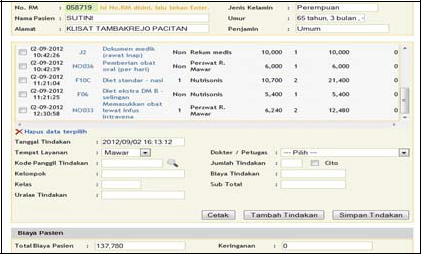
\includegraphics[width=12cm]{gambar/halaman_pembuatan_tagihan_billing.png}
		\caption{Rancangan halaman pembuatan tagihan billing. \\ Sumber: \citep{Gunawan2011sistem:11}}
		\label{Gambar:halamanpembuatantagihanbilling}
	\end{figure}
	
	\textbf{Gambar 2.26} menampilkan rancangan halaman pembuatan tagihan billing yang berisi \emph{field} No. RM, \emph{field} nama pasien, \emph{field} alamat, \emph{field} jenis kelamin, \emph{field} umur, \emph{field} penjamin, \emph{field} pilihan layanan atau barang yang digunakan, \emph{field} tanggal tindakan, \emph{field} tempat layanan, \emph{field} kode panggil tindakan, \emph{field} kelompok, \emph{field} kelas, \emph{field} uraian tindakan, \emph{field} dokter/petugas, \emph{field} jumlah tindakan, \emph{field} biaya tindakan, \emph{field} subtotal, \emph{field} total biaya pasien, \emph{field} keringanan beserta tombol cetak, tambah tindakan, dan simpan tindakan.
	
	\textbf{Gambar 2.27} pada halaman berikutnya menampilkan rancangan halaman pengelompokan penyakit berdasarkan icd yang berisi \emph{field} kode diagnosis ICD, \emph{field} diagnosis ICD, \emph{field} search, dan \emph{field} daftar penyakit beserta tombol tambah, koreksi, dan hapus.
	
	\begin{figure}[H]
		\centering
		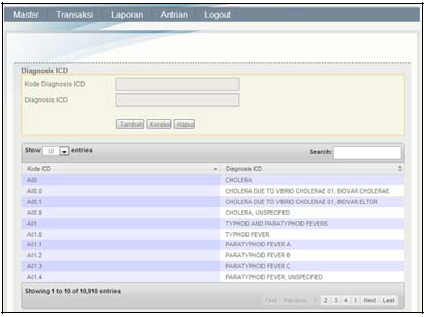
\includegraphics[width=12cm]{gambar/halaman_pengelompokan_penyakit_icd.png}
		\caption{Rancangan halaman pengelompokan penyakit berdasarkan ICD. \\ Sumber: \citep{Gunawan2011sistem:11}}
		\label{Gambar:halamanpengelompokanpenyakitberdasarkanicd}
	\end{figure}
	
	\begin{figure}[H]
		\centering
		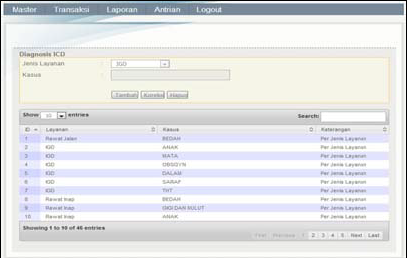
\includegraphics[width=12cm]{gambar/halaman_pengelompokan_kasus_penyakit_berdasarkan_poli.png}
		\caption{Rancangan halaman pengelompokan kasus penyakit berdasarkan poliklinik. \\ Sumber: \citep{Gunawan2011sistem:11}}
		\label{Gambar:halamanpengelompoankasuspenyakitberdasarkanpoliklinik}
	\end{figure}
	
	\textbf{Gambar 2.28} menampilkan rancangan halaman pengelompokan kasus penyakit berdasarkan poliklinik yang berisi \emph{field} jenis layanan, \emph{field} kasus, \emph{field} search, dan \emph{field} daftar layanan beserta tombol tambah, koreksi, dan hapus. 
	
	\begin{figure}[H]
		\centering
		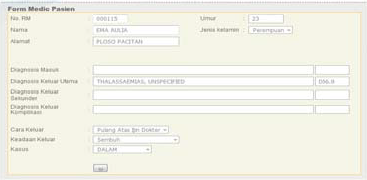
\includegraphics[width=12cm]{gambar/halaman_input_data_rekam_diagnosa.png}
		\caption{Rancangan halaman input form medis pasien. \\ Sumber: \citep{Gunawan2011sistem:11}}
		\label{Gambar:halamaninputformedispasien}
	\end{figure}
	
	\textbf{Gambar 2.29} menampilkan Rancangan halaman input form medis pasien yang berisi \emph{field} No. RM, \emph{field} nama, \emph{field} alamat, \emph{field} umur, \emph{field} jenis kelamin, \emph{field} diagnosa masuk, \emph{field} diagnosa keluar utama, \emph{field} diagnosa keluar sekunder, \emph{field} diagnosa keluar komplikasi, \emph{field} cara keluar, \emph{field} keadaan keluar, \emph{field} kasus, dan tombol ok.
	
	Dan berikut merupakan tampilan \emph{live} dari aplikasi \emph{web} jurnal kedua.
	
	\textbf{Gambar 2.30} pada halaman selanjutnya (A)menampilkan halaman \emph{login} yang berisi \emph{field} \emph{username}/\emph{email}, \emph{field} \emph{password}, tombol masuk, tombol \emph{login} dengan akun google, \emph{link} membuat akun baru, \emph{link} \emph{reset password}, dan \emph{link} bantuan. (B) menampilkan halaman registrasi yang berisi \emph{field} email, \emph{field username}, \emph{field} \emph{password}, \emph{field} nama lengkap, \emph{field} No. KTP, \emph{field} No. Telepon beserta tombol ceklis. Dan (C) menampilkan menu utama aplikasi yang berisi menu daftar \emph{online} rawat jalan, menu profil, menu rawat inap, menu dokter, menu rawat jalan, menu penunjang, menu galeri, menu daftar \emph{online}, menu efek samping obat, menu info kamar, menu telepon, menu akun, dan menu lainnya.
	
	\begin{figure}[H]
		\centering
		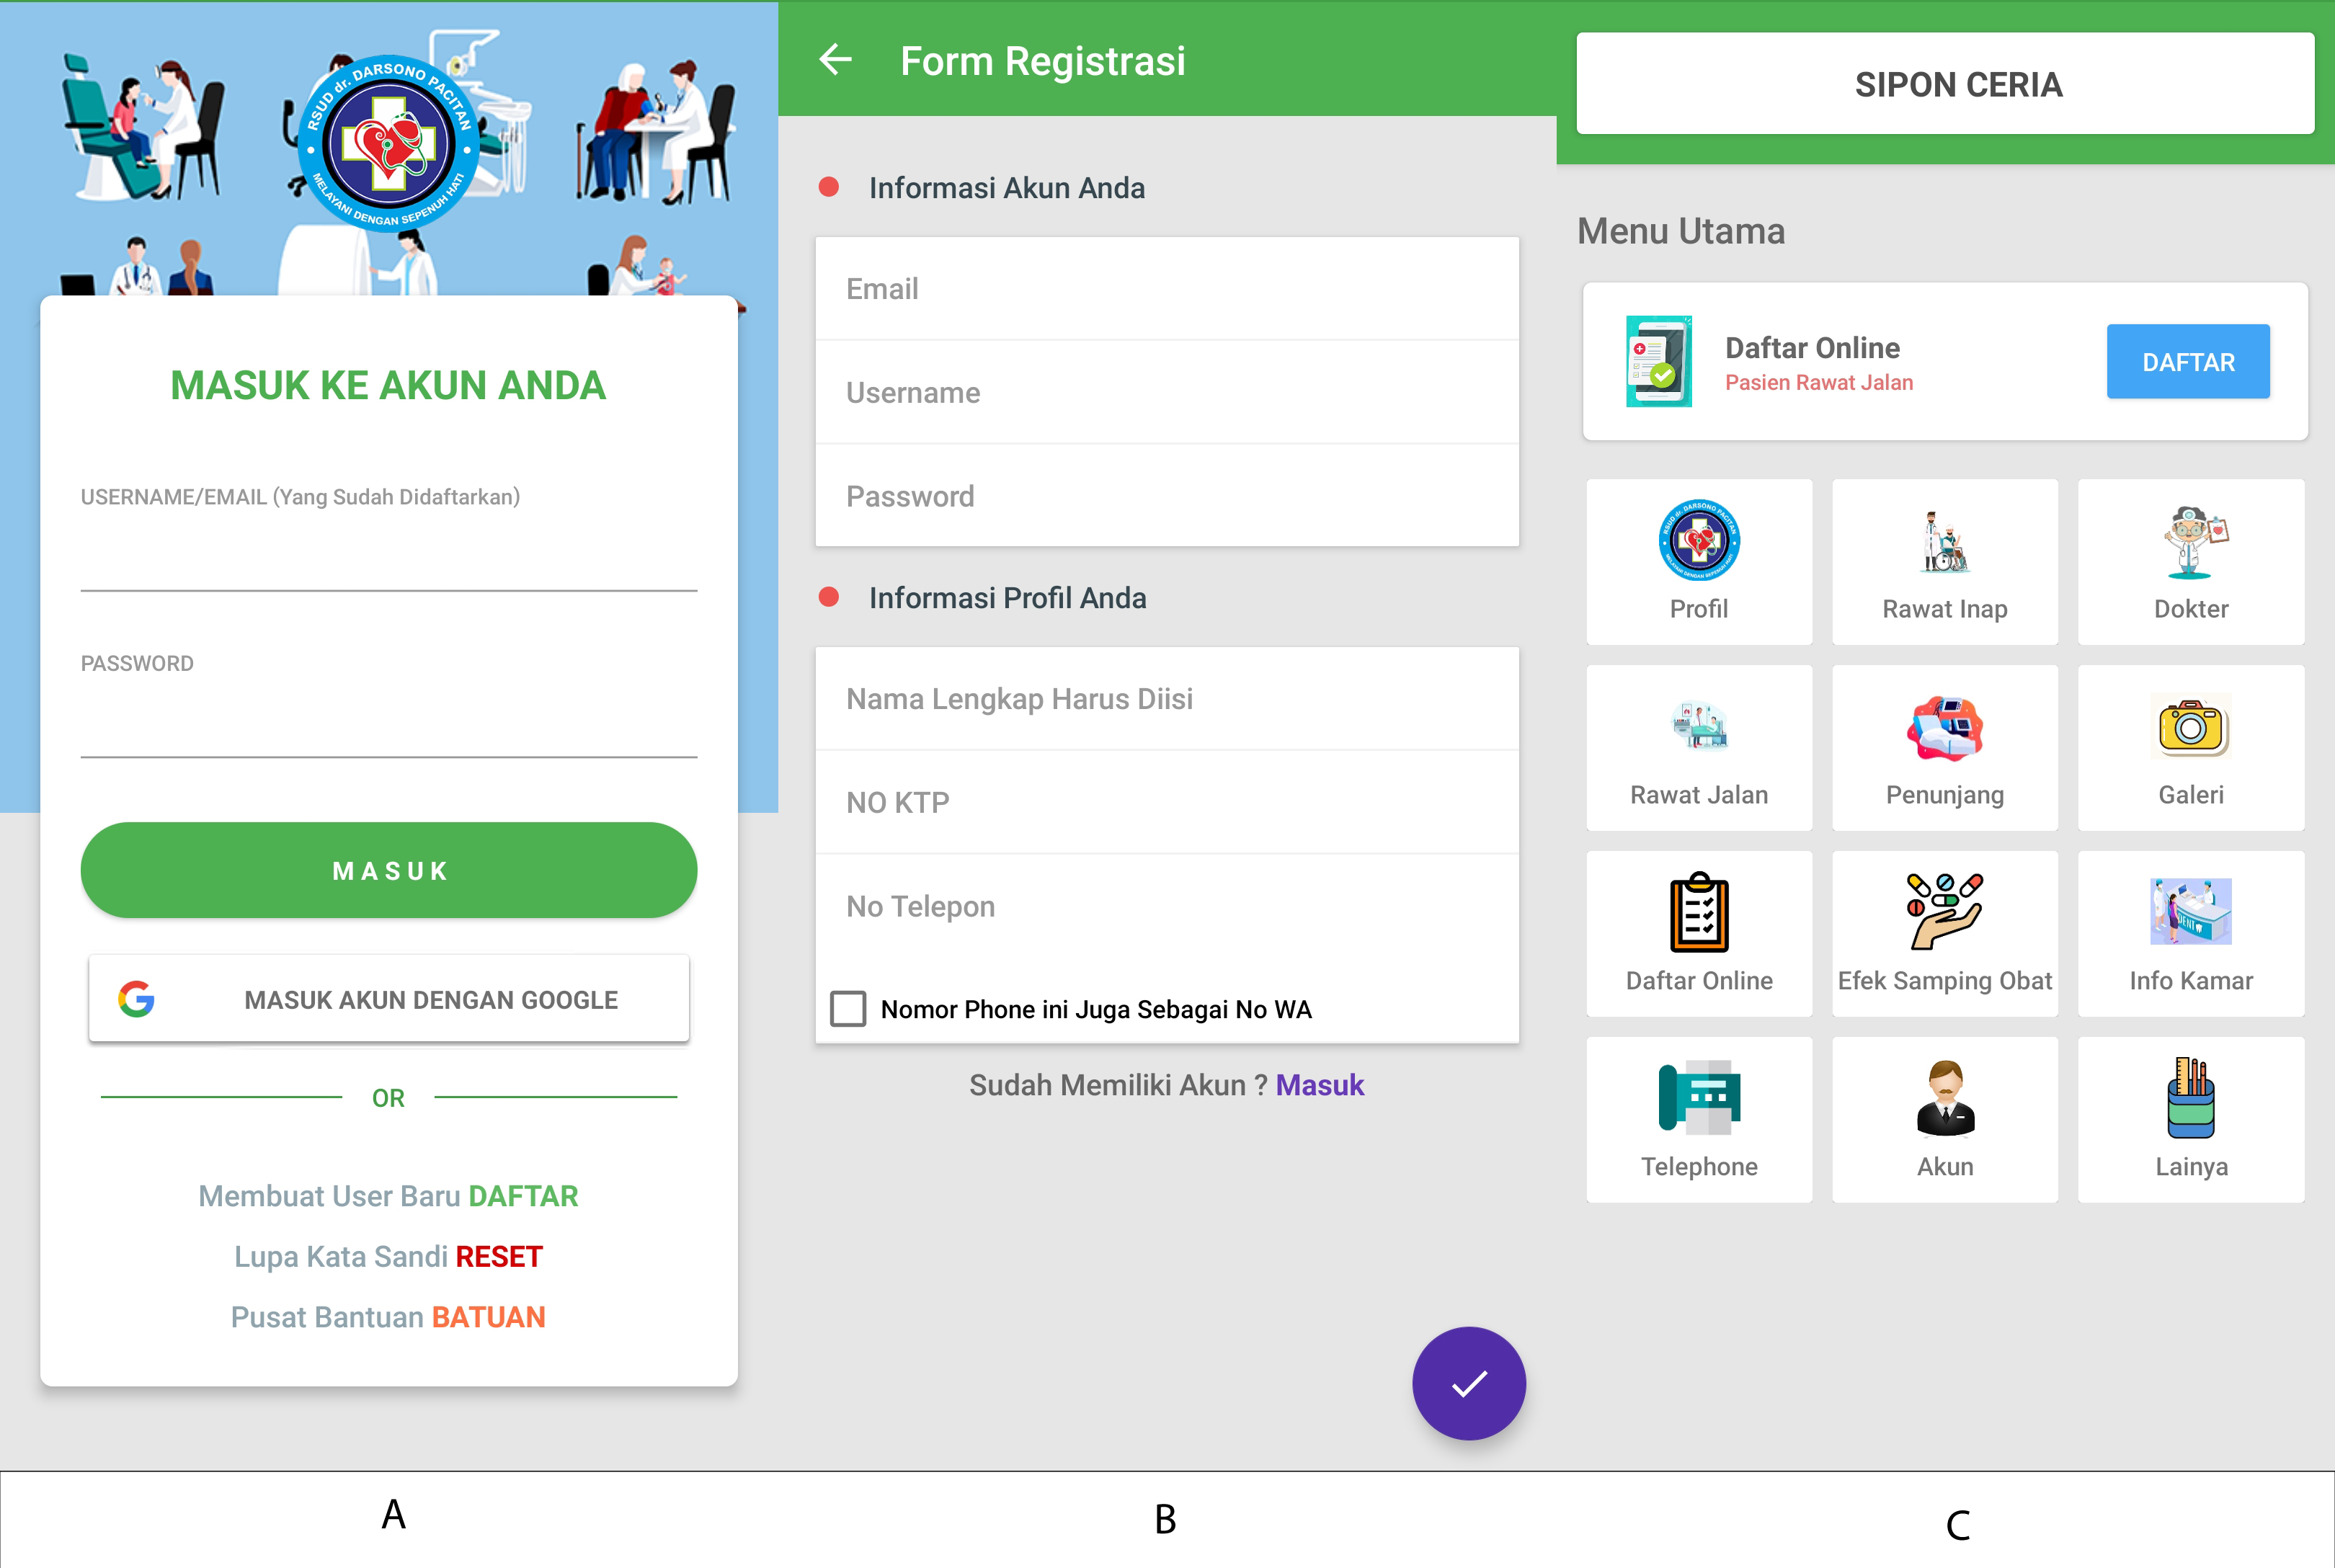
\includegraphics[width=12cm]{gambar/1.jpg}
		\caption{(A) Halaman login. (B)Halaman registrasi. (C)Halaman awal. \\ Sumber: Aplikasi android SIPON CERIA}
		\label{Gambar:halamanlive0jurnal2}
	\end{figure}
	
	\textbf{Gambar 2.31} pada halaman selanjutnya (A)menampilkan halaman input data pasien yang berisi \emph{field} hubungan dengan keluarga, \emph{field} No. RM, \emph{field} tanggal lahir pasien, \emph{field} No. Telepon, \emph{field} email, dan \emph{field} No. KTP. (B) menampilkan halaman bukti pendaftaran pasien. Dan (C) menampilkan halaman riwayat daftar \emph{online}.
	
	\begin{figure}[H]
		\centering
		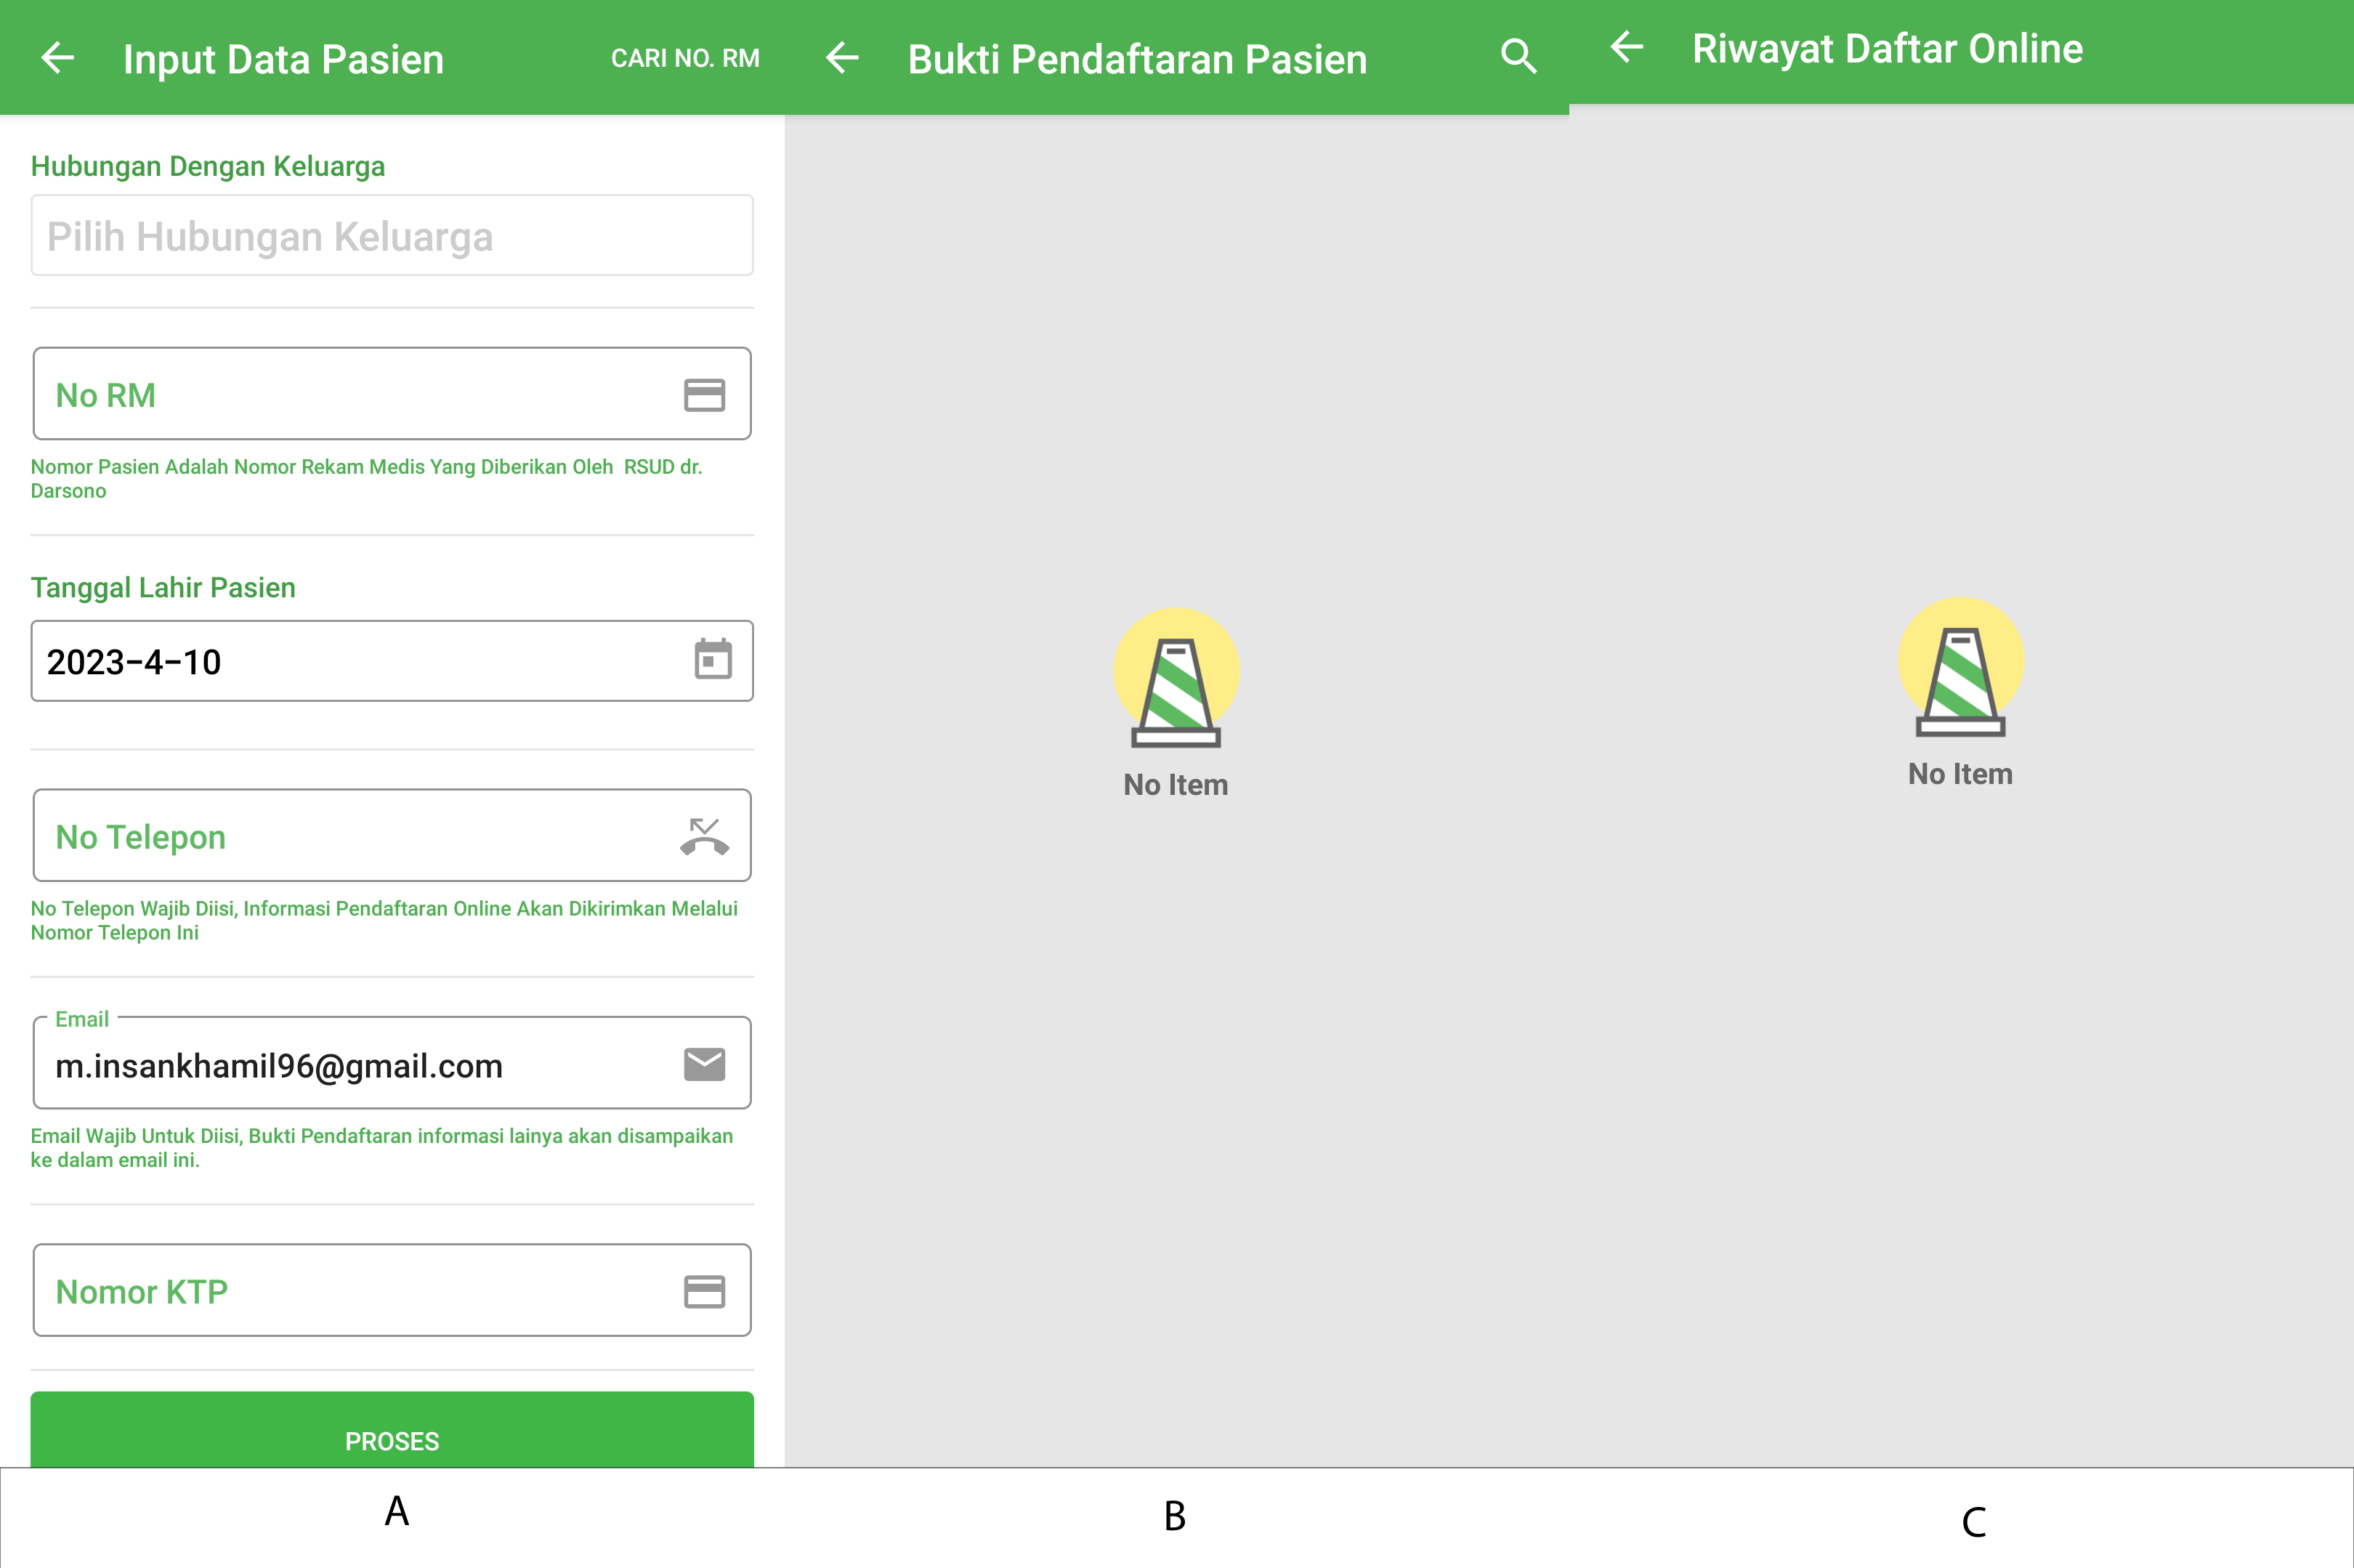
\includegraphics[width=12cm]{gambar/2.jpg}
		\caption{(A) Halaman \emph{input} data pasien. (B) Halaman bukti pendaftaran pasien. (C) Halaman riwayat daftar pasien. \\ Sumber: Aplikasi android SIPON CERIA}
		\label{Gambar:halamanlive1jurnal2}
	\end{figure}
	
	
	\begin{figure}[H]
		\centering
		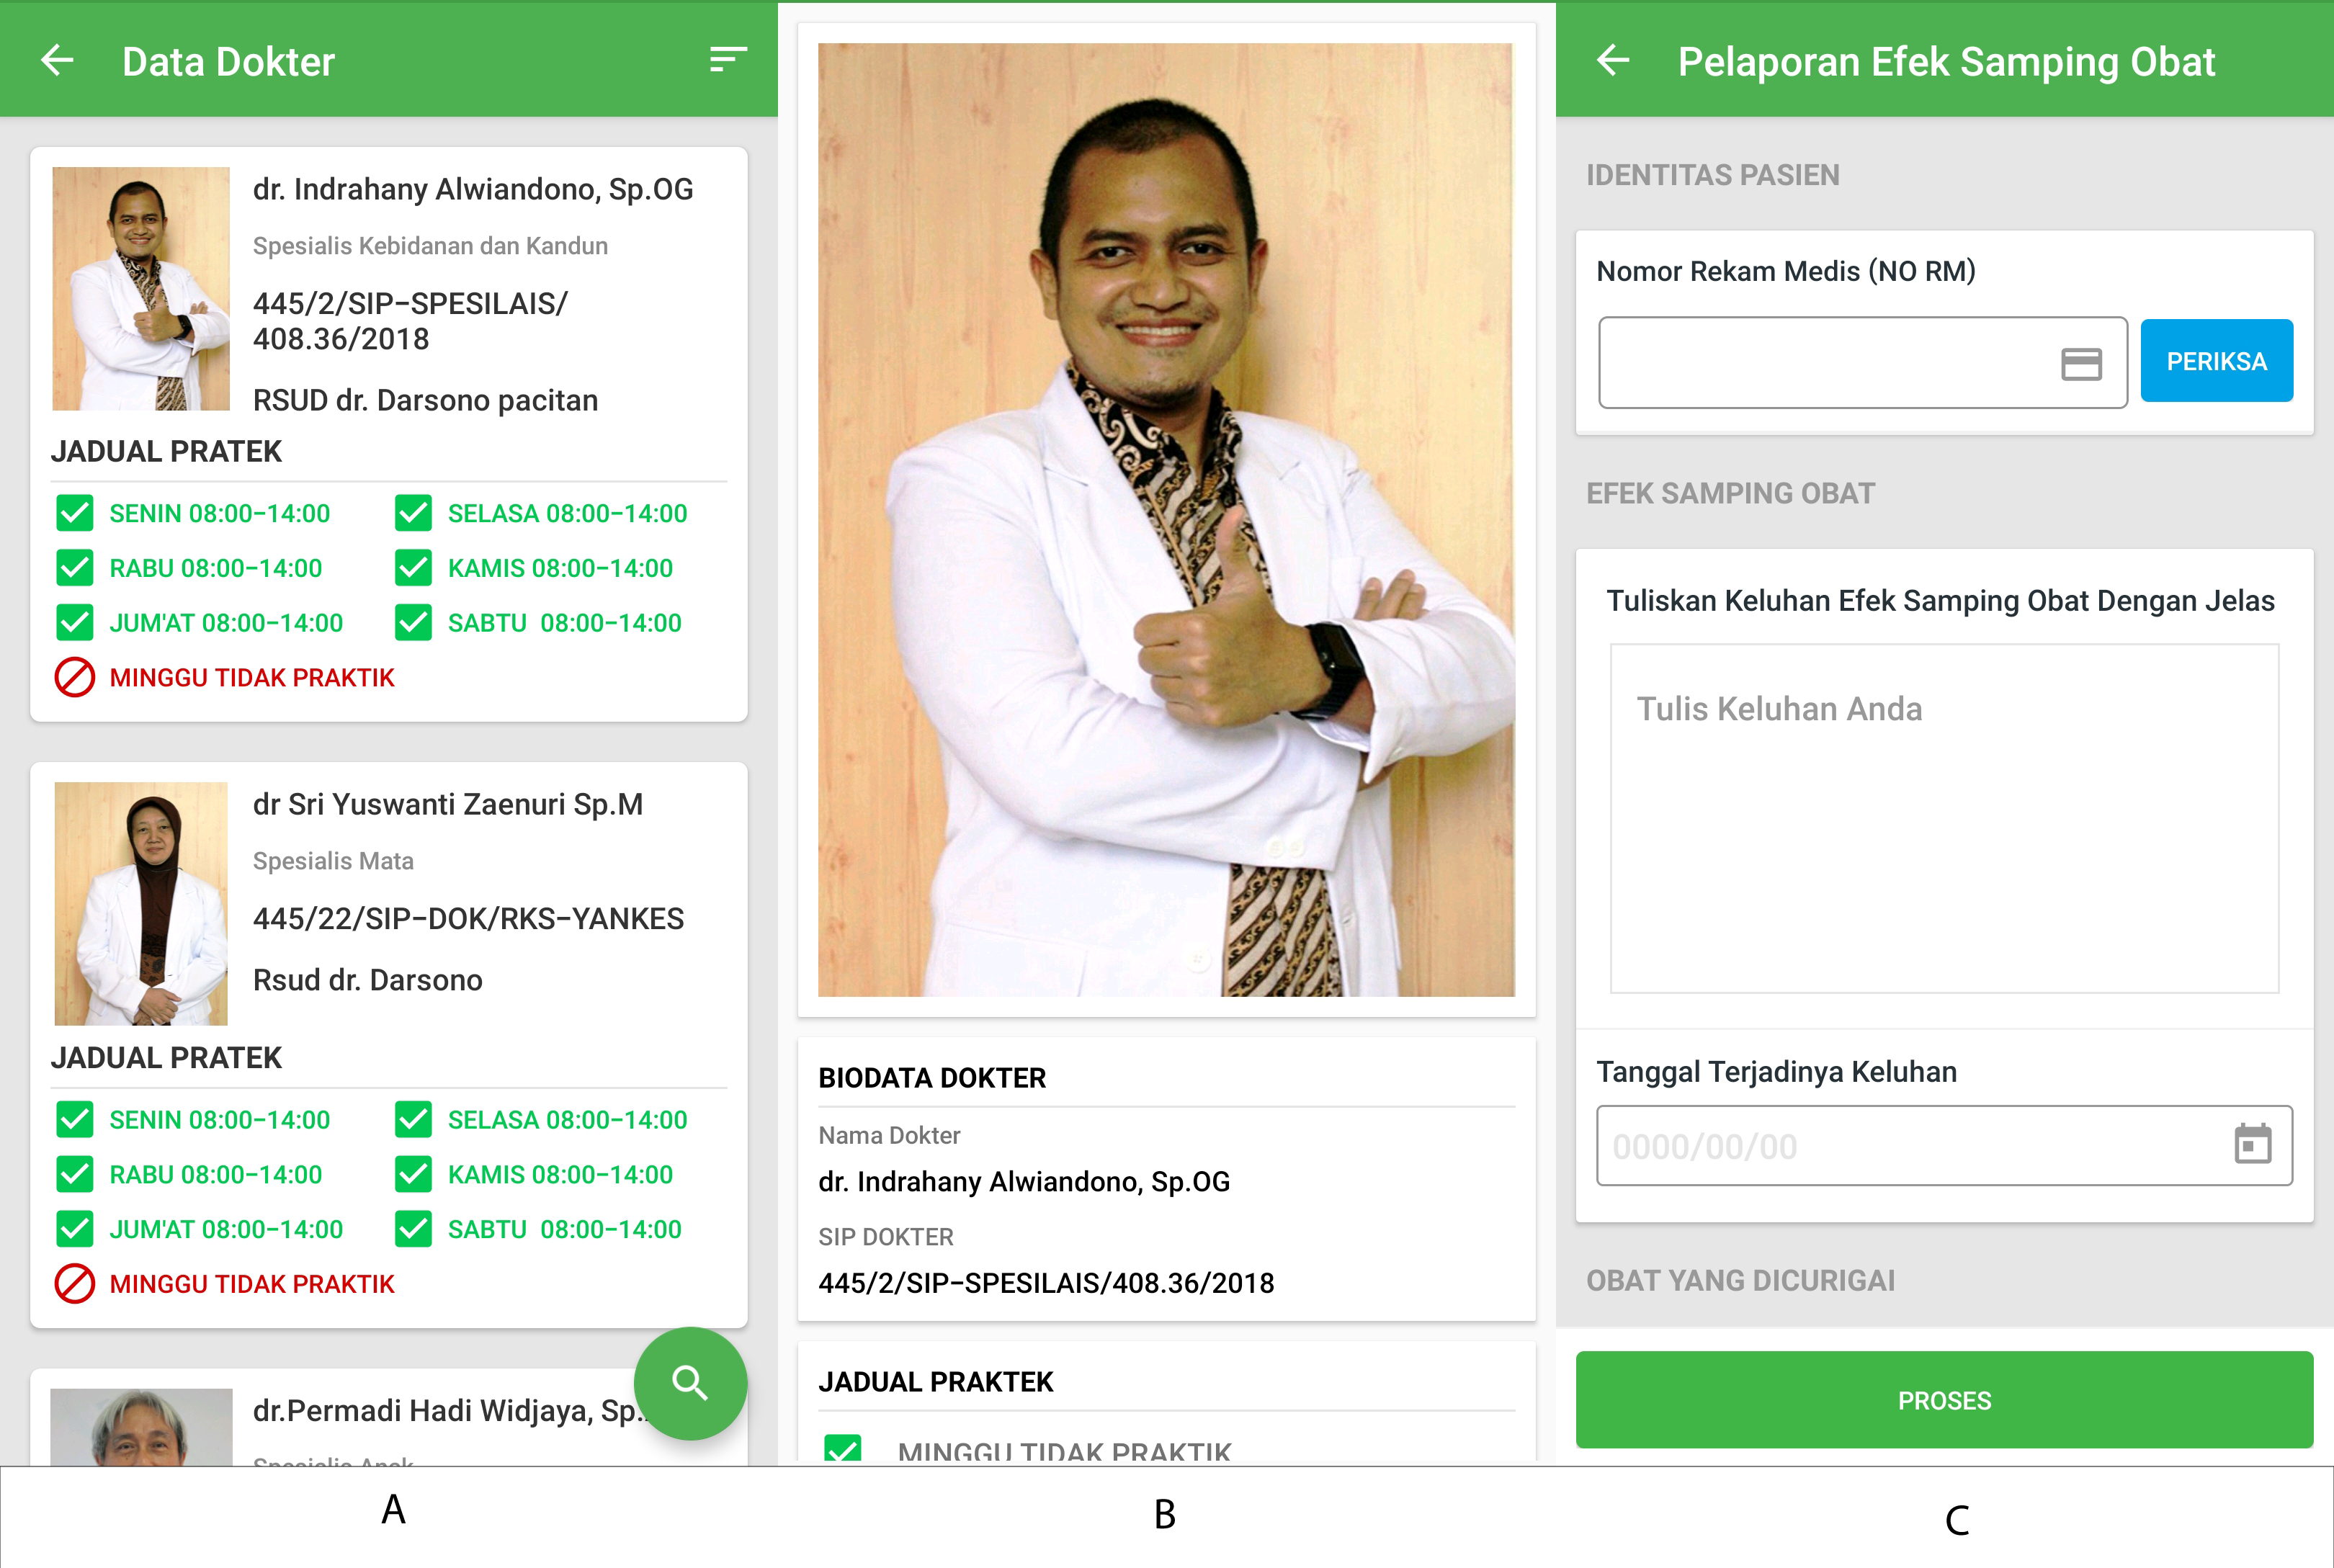
\includegraphics[width=12cm]{gambar/3.jpg}
		\caption{(A) Halaman \emph{list} dokter. (B) Halaman detail data dokter. (C) Halaman menu pelaporan efek samping obat. \\ Sumber: Aplikasi android SIPON CERIA}
		\label{Gambar:halamanlive2jurnal2}
	\end{figure}
	
	\textbf{Gambar 2.32} (A)menampilkan halaman \emph{list} dokter yang berisi \emph{list} dokter yang tersedia lengkap dengan foto, nama, spesialis bidang, dan jadwal praktek. (B) menampilkan halaman detail data dokter yang berisi biodata dokter lengkap. Dan (C) menampilkan halaman menu pelaporan efek samping obat yang berisi \emph{field} No. RM, \emph{field} keluhan efek samping, \emph{field} tanggal terjadinya keluhan dan \emph{field} nama obat yang dicurigai.
	
	\textbf{Gambar 2.33} (A)menampilkan halaman menu rawat jalan yang berisi \emph{list} poliklinik beserta jadwal pelayanan. (B) menampilkan halaman \emph{list} data dokter yang berkaitan dengan poliklinik yang dipilih. Dan (C) menampilkan halaman \emph{list} fasilitas poliklinik yang dipilih.
	
	\begin{figure}[H]
		\centering
		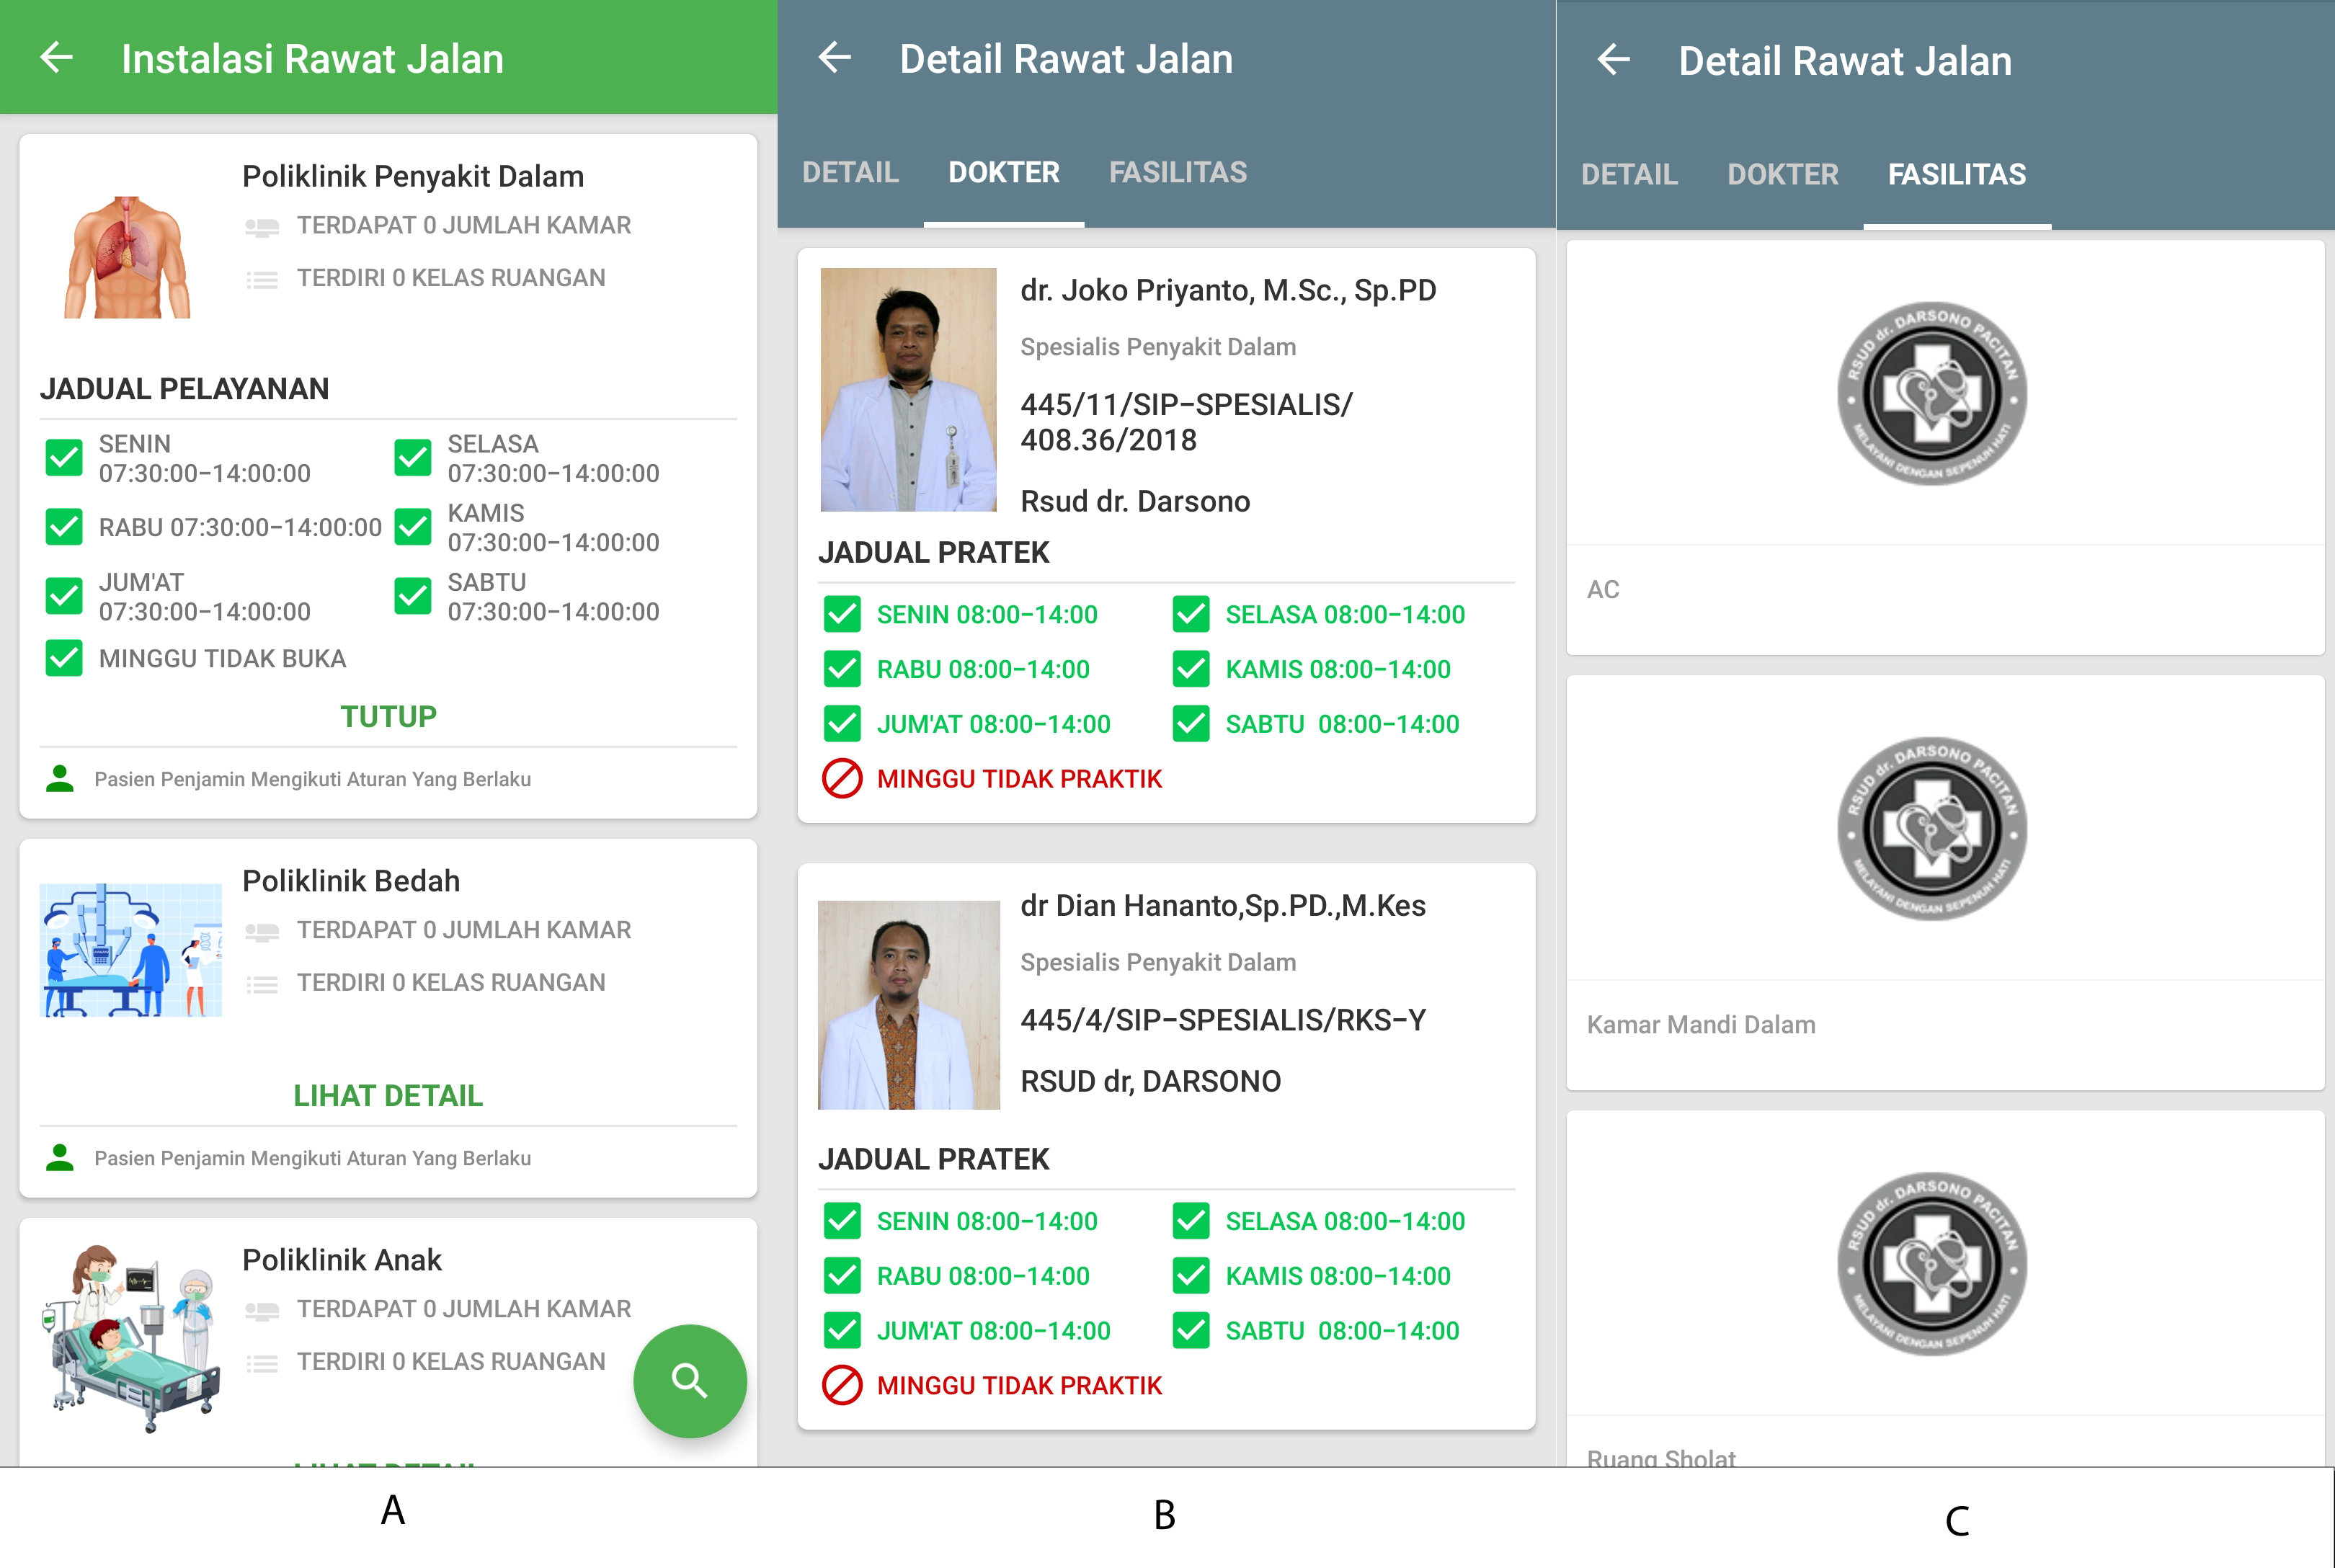
\includegraphics[width=12cm]{gambar/4.jpg}
		\caption{(A) Halaman menu rawat jalan. (B) Halaman detail rawat jalan \emph{list} dokter. (C) Halaman detail rawat jalan \emph{list} fasilitas. \\ Sumber: Aplikasi android SIPON CERIA}
		\label{Gambar:halamanlive3jurnal2}
	\end{figure}
	
	\begin{figure}[H]
		\centering
		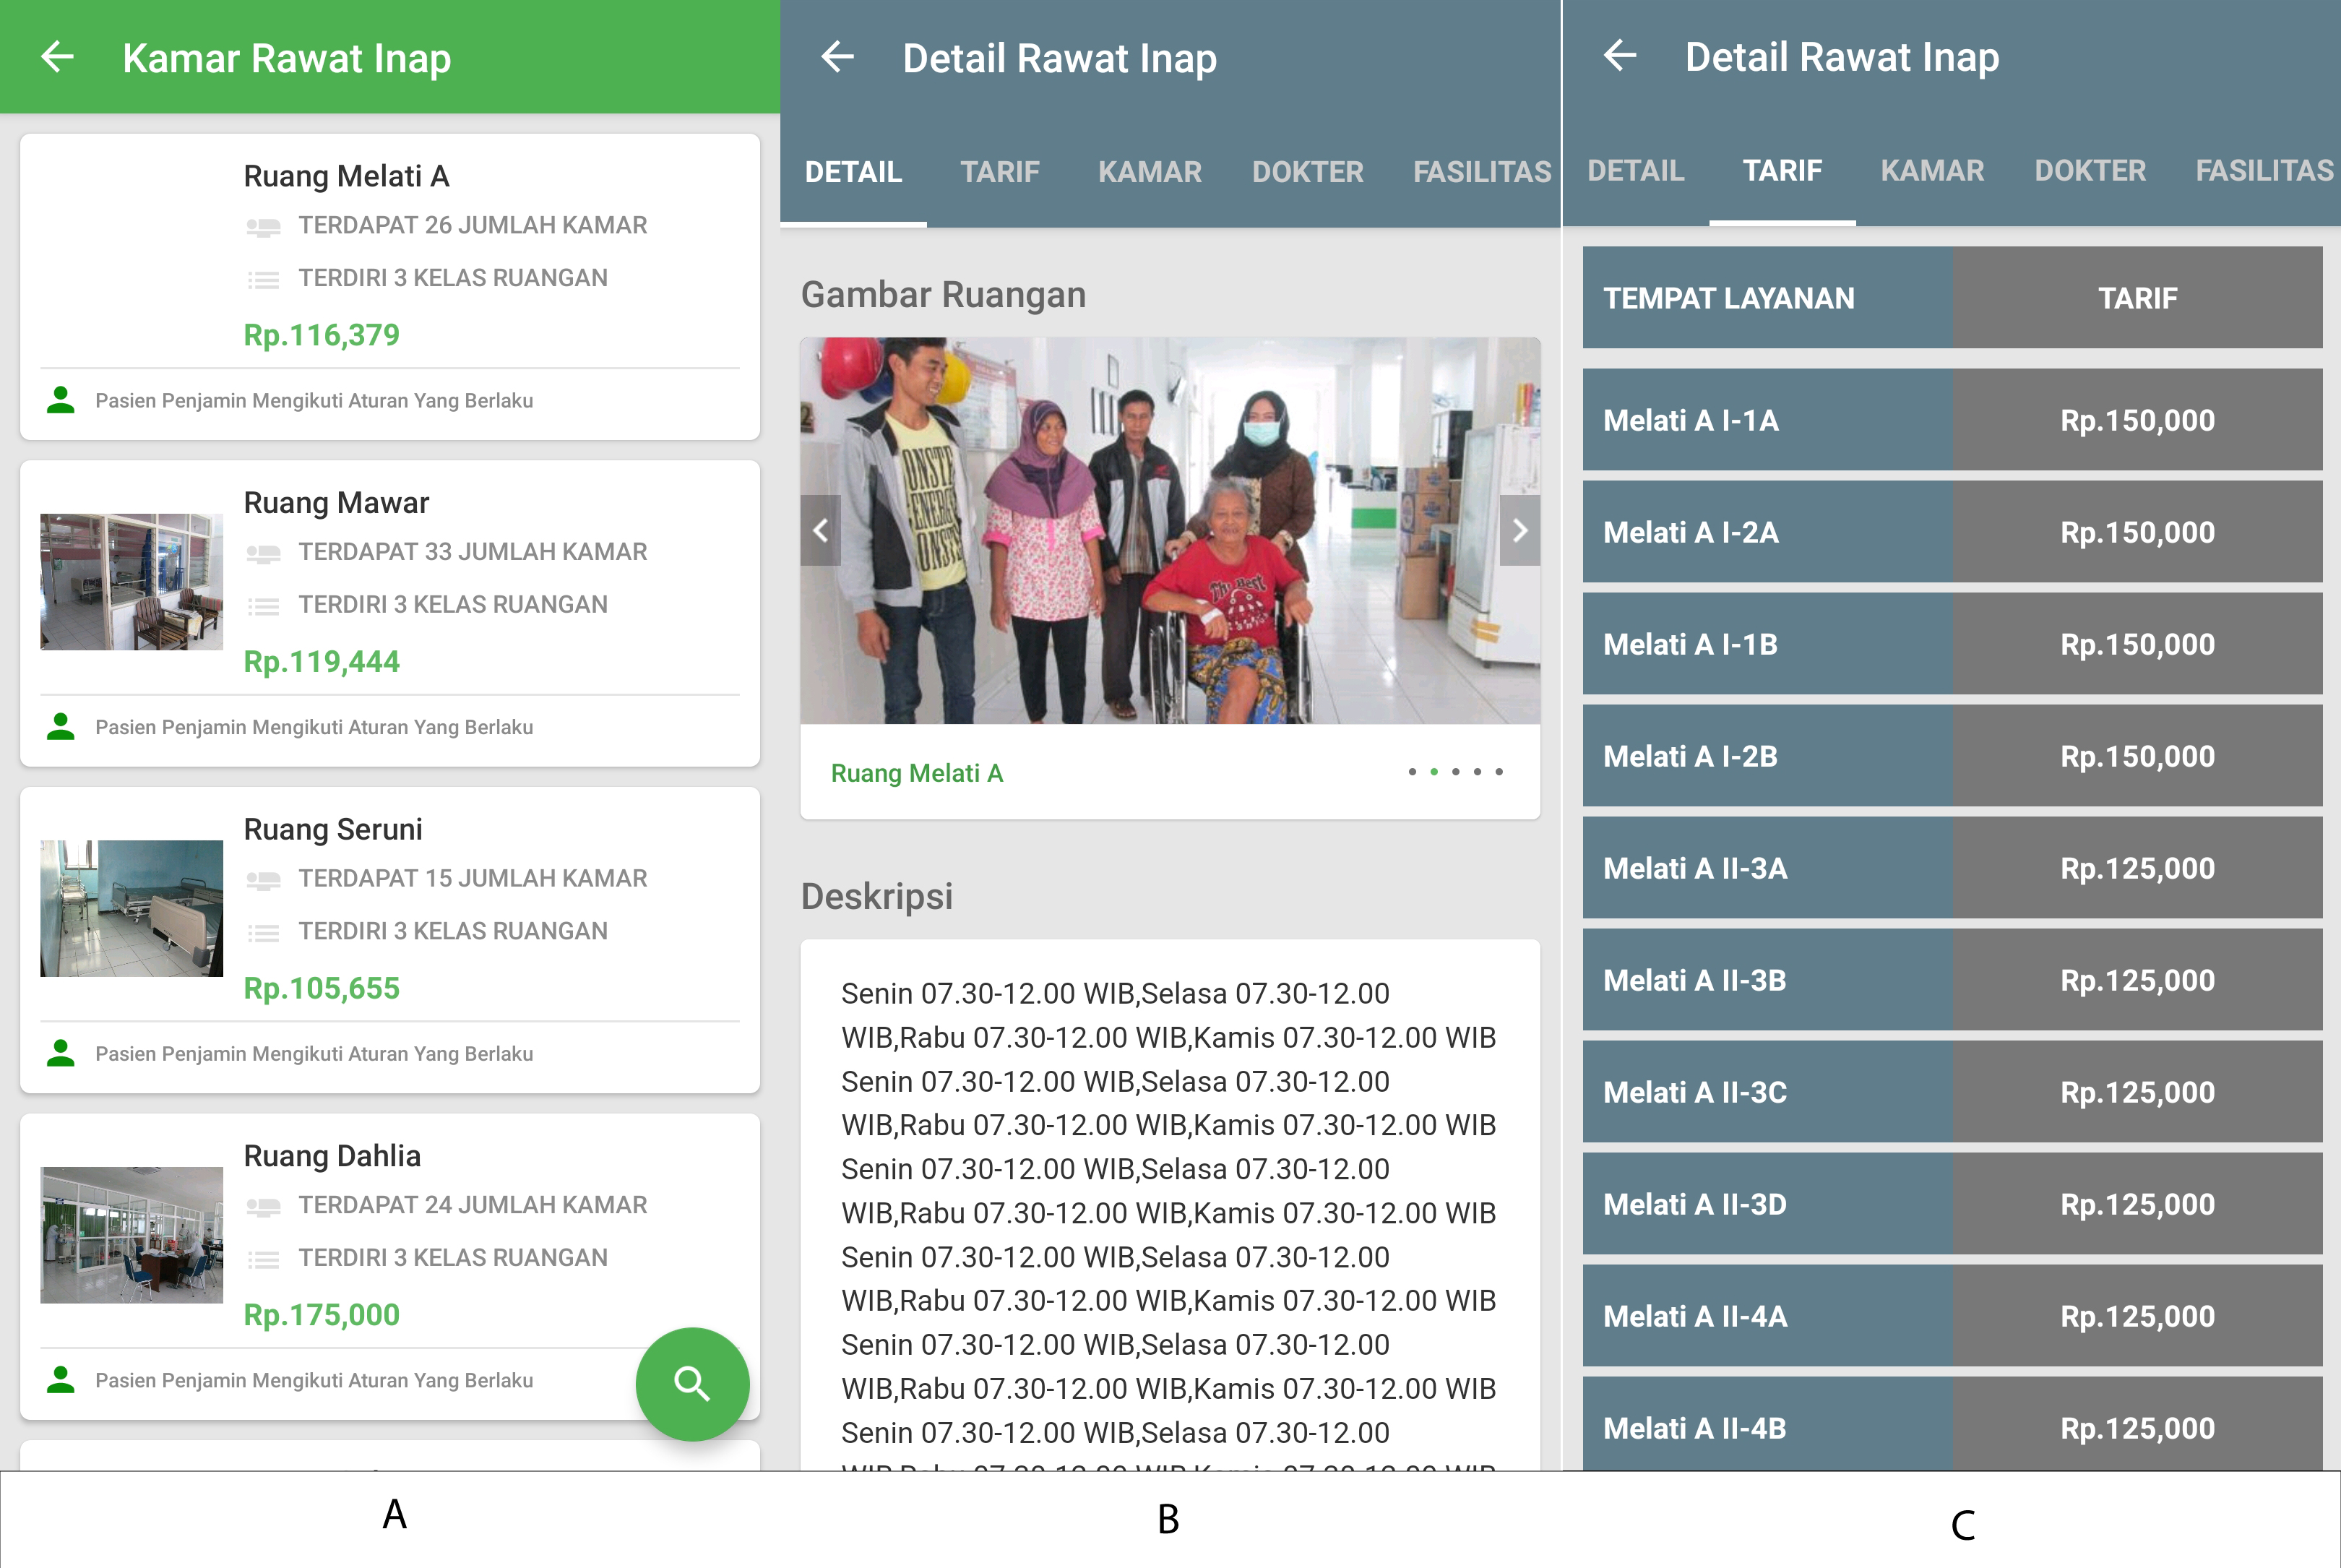
\includegraphics[width=12cm]{gambar/5.jpg}
		\caption{(A) Halaman menu rawat inap. (B) Halaman detail rawat inap detail. (C) Halaman detail rawat inap \emph{list} tarif. \\ Sumber: Aplikasi android SIPON CERIA}
		\label{Gambar:halamanlive4jurnal2}
	\end{figure}
	
	\textbf{Gambar 2.34} (A)menampilkan halaman menu rawat inap yang berisi \emph{list} ruang rawat inap beserta foto ruangan dan harganya. (B) menampilkan halaman detail ruang rawat inap yang dipilih. Dan (C) menampilkan halaman \emph{list} harga ruangan rawat inap yang dipilih sesuai kelas.
	
	\textbf{Gambar 2.35} pada halaman selanjutnya (A)menampilkan halaman \emph{list} ruang rawat inap berdasarkan kelas, detail dan harganya. (B) menampilkan halaman \emph{list} dokter yang berkaitan dengan rawat inap . Dan (C) menampilkan halaman \emph{list} fasilitas ruangan rawat inap yang dipilih.
	
	\begin{figure}[H]
		\centering
		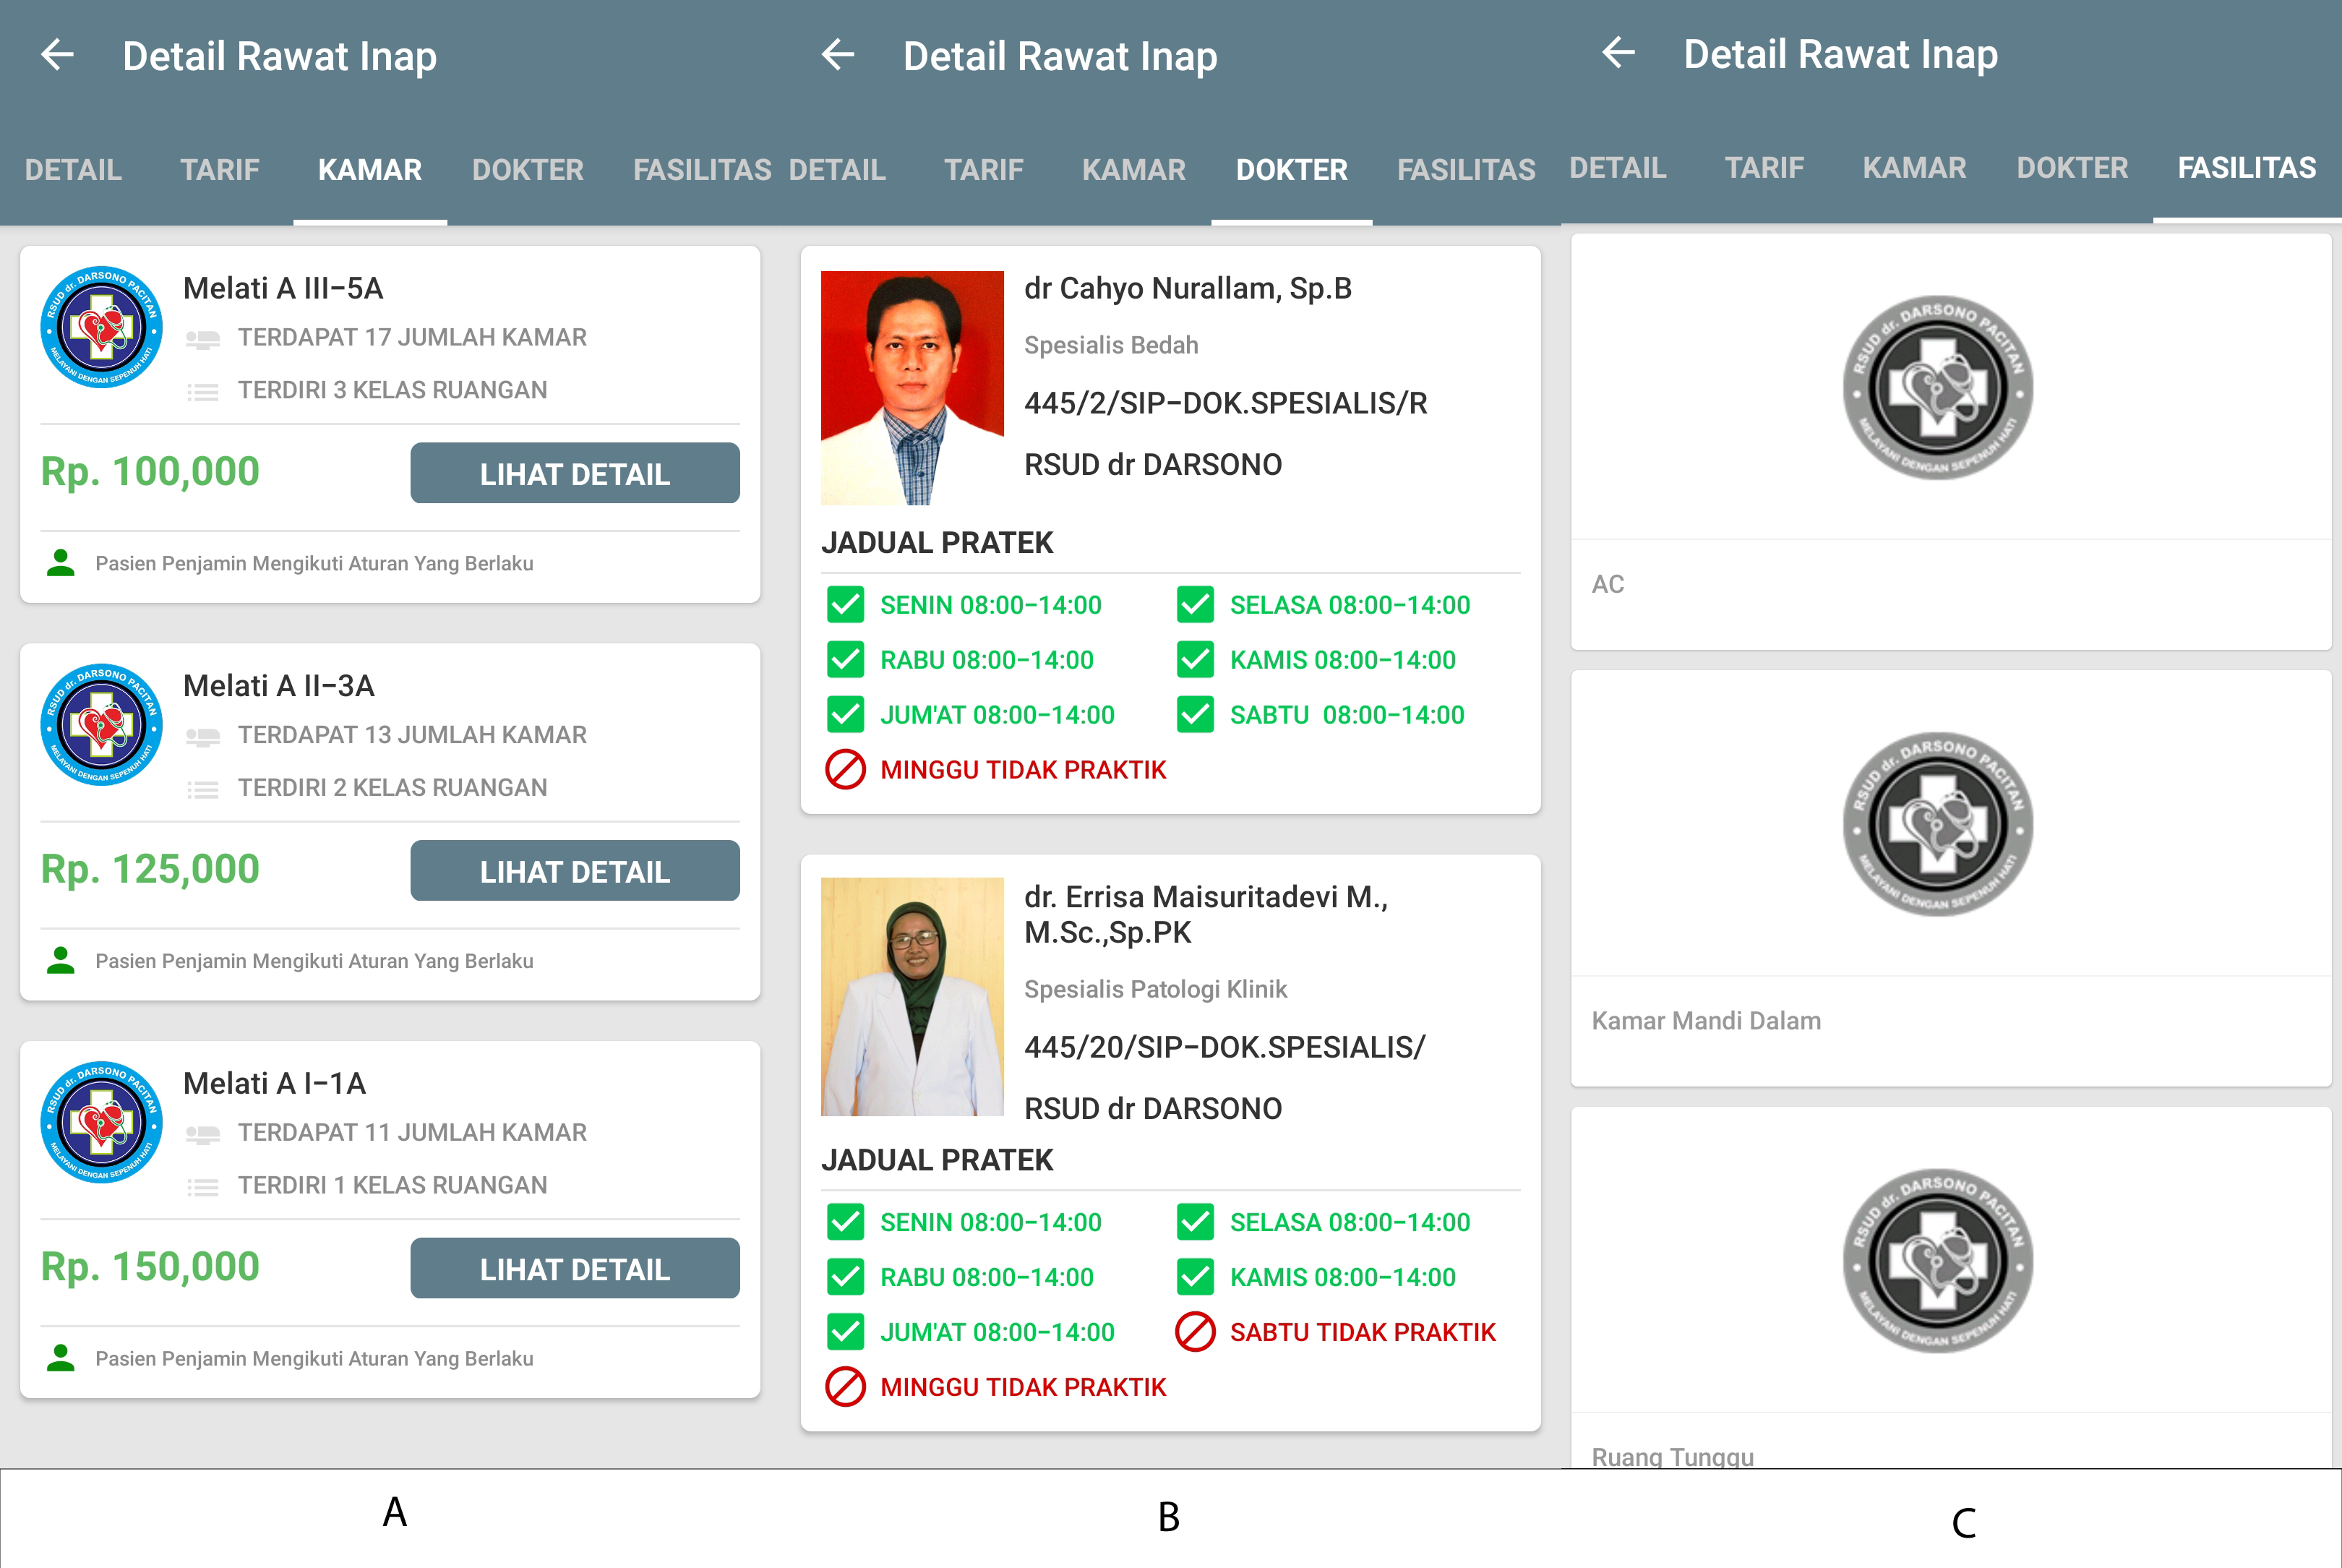
\includegraphics[width=12cm]{gambar/6.jpg}
		\caption{(A) Halaman detail rawat inap \emph{list} kamar. (B) Halaman detail rawat inap \emph{list} dokter. (C) Halaman \emph{list} fasilitas ruangan rawat inap. \\ Sumber: Aplikasi android SIPON CERIA}
		\label{Gambar:halamanlive5jurnal2}
	\end{figure}
	
	\item UI/UX pada jurnal ketiga
	
	Berikut di bawah ini merupakan UI/UX yang ditampilkan didalam jurnal ketiga. Pada jurnal ini hanya ditampilkan satu dari 12 UI/UX, yaitu halaman membuat reservasi.
	
	\textbf{Gambar 2.36} pada halaman selanjutnya menampilkan Rancangan halaman membuat reservasi berobat yang berisi \emph{field} nama pasien, \emph{field} jenis kelamin, \emph{field} tempat lahir, \emph{field} tanggal lahir, \emph{field} umur, \emph{field} status pernikahan, \emph{field} tanggal reservasi, \emph{field} pekerjaan, \emph{field} alamat lengkap, \emph{field} kecamatan.
	
	\begin{figure}[H]
		\centering
		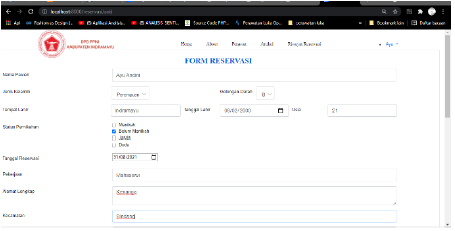
\includegraphics[width=12cm]{gambar/halaman_membuat_reservasi.png}
		\caption{Rancangan halaman membuat reservasi \emph{online} \\ Sumber: \cite{Carminah2021aplikasi:12}}
		\label{Gambar:halamanmembuatreservasionline}
	\end{figure}
	
	Dan pada jurnal ketiga tidak ditemukan \emph{website live}-nya.
	
\end{enumerate}

\subsection{Kesimpulan Studi Banding}

Tabel di bawah ini merupakan tabel fitur sistem informasi rumah sakit berdasarkan 3 jurnal yang telah peneliti sebutkan sebelumnya.

\begin{table}[H]
	\centering
	\caption{Tabel fitur sistem informasi rumah sakit}
	\label{tabel_input}
	\begin{tabular}{|c|m{7cm}|c|c|c|}
		\hline
		\textbf{No} & \textbf{Fitur} & \textbf{Jurnal 1} & \textbf{Jurnal 2} & \textbf{Jurnal 3} \\
		\hline
		
		& 
		\textbf{Dari sisi pasien} &
		& &\\
		\hline 
		
		1& 
		Melihat data dokter                      
		(pasien dapat melihat detail data dokter) &
		\tickYes& &\\
		\hline
		
		2& 
		Melihat jadwal dokter
		(pasien dapat melihat jadwal dokter) &
		\tickYes& &\\
		\hline
		
		3 & 
		Melihat jumlah pasien yang telah nendaftar berobat
		(pasien dapat melihat pasien lain yang telah daftar berobat) &
		\tickYes& &\\
		\hline
		
	\end{tabular}
\end{table}

\begin{table}[H]
	\centering
	\caption{Fitur sistem informasi rumah sakit - lanjutan 1}
	\label{tabel_input}
	\begin{tabular}{|c|m{7cm}|c|c|c|}
		\hline
		\textbf{No} & \textbf{Fitur} & \textbf{Jurnal 1} & \textbf{Jurnal 2} & \textbf{Jurnal 3} \\
		\hline
		
		& 
		\textbf{Dari sisi pasien} &
		& &\\
		\hline
		
		4 & 
		Pasien bisa mengelola akun sendiri
		(pasien dapat membuat dan merubah akun \emph{online} secara mandiri) &
		& \tickYes &\\
		\hline
		
		5 & 
		Melakukan pendaftaran berobat secara \emph{online}
		(pasien dapat melakukan pendaftaran berobat \emph{online}) &
		\tickYes& \tickYes &\\
		\hline
		
		6 & 
		Melihat notifikasi sms nomor antrian berobat
		(pasien mendapatkan sms dan dapat mengetahui nomor antrian berobatnya) &
		\tickYes& &\\
		\hline
		
		7 & 
		Melihat status berobat (pasien dapat melihat status berobat mereka yaitu sudah diverifikasi, belum diverifikasi, \emph{cancel})&
		\tickYes & &\\
		\hline
		
		& 
		\textbf{Dari sisi pegawai rumah sakit} &
		& &\\
		\hline
		
		8 & 
		Mengelola akun pasien (pegawai rumah sakit dapat menambah, menghapus, merubah akun pasien) &
		\tickYes & \tickYes &\\
		\hline
		
		9 & 
		Mengelola akun pegawai rumah sakit (pegawai rumah sakit dapat menambah, menghapus, merubah akun pegawai rumah sakit) &
		\tickYes & & \tickYes \\
		\hline
		
	\end{tabular}
\end{table}

\begin{table}[H]
	\centering
	\caption{Tabel fitur sistem informasi rumah sakit - lanjutan 2}
	\label{tabel_input}
	\begin{tabular}{|c|m{7cm}|c|c|c|}
		\hline
		\textbf{No} & \textbf{Fitur} & \textbf{Jurnal 1} & \textbf{Jurnal 2} & \textbf{Jurnal 3} \\
		\hline
		
		& 
		\textbf{Dari sisi pegawai rumah sakit} &
		& &\\
		\hline
		
		10 & 
		Mendaftarkan pasien berobat (pegawai rumah sakit dapat mendaftarkan pasien berobat secara \emph{offline} di tempat) &
		& \tickYes &\\
		\hline
		
		11 & 
		Mengelola status pasien berobat (pegawai rumah sakit dapat memberikan status verifikasi atau \emph{cancel}) &
		\tickYes& & \tickYes \\
		\hline
		
		12 & 
		Membuat data rekam medis pasien (pegawai rumah sakit dapat membuat laporan data rekam medis pasien yang telah berobat) &
		& \tickYes & \tickYes \\
		\hline
		
		13 & 
		Mengelola jadwal dokter (pegawai rumah sakit dapat menambah dan merubah jadwal praktik dokter sesuai kebutuhan) &
		\tickYes& &\\
		\hline
		
		14 & 
		Mengelola jadwal dokter (pegawai rumah sakit dapat menambah dan merubah jadwal praktik dokter sesuai kebutuhan) &
		\tickYes& &\\
		\hline
		
		15 & 
		Mengelola inventaris rumah sakit (pegawai rumah sakit dapat menambah \emph{item}, menghapus \emph{item}, merubah \emph{item}, mengurangi kuantitas \emph{item}, menambah kuantitas \emph{item} inventaris rumah sakit)  &
		& \tickYes &\\
		\hline
		
	\end{tabular}
\end{table}

\begin{table}[H]
	\centering
	\caption{Tabel fitur sistem informasi rumah sakit - lanjutan 3}
	\label{tabel_input}
	\begin{tabular}{|c|m{7cm}|c|c|c|}
		\hline
		\textbf{No} & \textbf{Fitur} & \textbf{Jurnal 1} & \textbf{Jurnal 2} & \textbf{Jurnal 3} \\
		\hline
		
		& 
		\textbf{Dari sisi pegawai rumah sakit} &
		& &\\
		\hline
		
		16 & 
		Membuat \emph{bill} tagihan pasien rumah sakit (pegawai rumah sakit dapat membuat \emph{bill} tagihan total baik layanan maupun \emph{item} yang telah digunakan pasien) &
		& \tickYes &\\
		\hline
		
		17 & 
		Mengelola artikel (pegawai rumah sakit dapat menambah, menghapus, merubah artikel yang dipublikasi pada laman \emph{web} rumah sakit)&
		&  & \tickYes \\
		\hline
		
		& 
		\textbf{Dari sisi aplikasi} &
		& &\\
		\hline
		
		18 & 
		Aplikasi sudah ter-\emph{deploy} &
		& \tickYes &\\
		\hline
		
	\end{tabular}
\end{table}

Peneliti melakukan perhitungan angka persentase fitur yang ter-\emph{deploy} terhadap rancangan fitur yang ada pada jurnal. Dan didapat hasilnya dibawah ini:

\textbf{Persentase fitur yang ter-\emph{deploy} pada jurnal pertama}

0/6 = \textbf{0\%}

ada 0 dari 6 rancangan fitur yang ter-\emph{deploy}.

\textbf{Persentase fitur yang ter-\emph{deploy} pada jurnal kedua}

1/6 = \textbf{16,7\%}

ada 1 dari 6 rancangan fitur yang ter-\emph{deploy}.

\textbf{Persentase fitur yang ter-\emph{deploy} pada jurnal ketiga}

0/4 = \textbf{0\%}

ada 0 dari 4 rancangan fitur yang ter-\emph{deploy}.

Peneliti juga melakukan perhitungan angka persentase UI/UX yang terealisasi terhadap rancangan UI/UX yang terdapat pada jurnal.

\textbf{Persentase UI/UX yang terealisasi pada jurnal pertama}

0/5 = \textbf{0\%}

ada 0 dari 5 rancangan UI/UX yang terealisasi.

\textbf{Persentase UI/UX yang terealisasi pada jurnal kedua}

0/6 = \textbf{0\%}

ada 0 dari 6 rancangan UI/UX yang terealisasi.

\textbf{Persentase UI/UX yang terealisasi pada jurnal ketiga}

0/1 = \textbf{0\%}

ada 0 dari 1 rancangan UI/UX yang terealisasi.

Pada aplikasi \emph{web} pada jurnal 1 hanya terdapat \emph{landing page web} dan aplikasi rancangan \emph{web} sesuai jurnal 1 belum ter-\emph{deploy} hingga saat ini sehingga belum bisa digunakan. Karena belum ter-\emph{deploy} maka UI/UX pada saat perancangan didalam jurnal belum ada yang terealisasi.

Selanjutnya aplikasi \emph{web} kedua hanya ada 1 fitur yang ter-\emph{deploy} yaitu melakukan pendaftaran berobat secara online oleh pasien. Namun UI/UX pada saat perancangan dan \emph{live} berbeda. 

Dan pada aplikasi \emph{web} ketiga tidak ditemukan \emph{website live}-nya sehingga dapat diartikan aplikasi rancangan \emph{web} sesuai jurnal 3 belum ter-\emph{deploy} hingga saat ini dan belum bisa digunakan. 

Dengan begitu peneliti menarik kesimpulan bahwa dalam praktik perancangan sebuah \emph{website} terdapat perbedaan antaran praktik(perancangan) dan realita.
\end{comment}

%!TEX root = ./template-skripsi.tex
%-------------------------------------------------------------------------------
%                            BAB III
%               			PEMBAHASAN
%-------------------------------------------------------------------------------

\chapter{METODOLOGI PENELITIAN}

Melalui penelitian yang dilakukan oleh penulis, akan menghasilkan produk tertentu. Penelitian yang dilakukan oleh penulis juga termasuk dalam jenis penelitian dan pengembangan. Berikut adalah tahapan-tahapan penelitian yang penulis lakukan dalam perancangan sebuah aplikasi:

\begin{figure}[H]
	\centering
	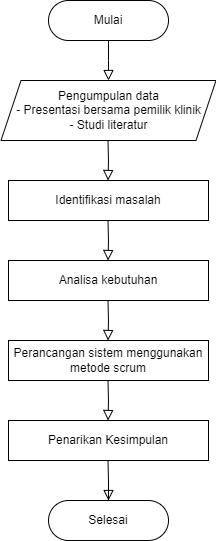
\includegraphics[width=4cm]{gambar/tahapan penelitian fix.png}
	\caption{Tahapan penelitian} 
	\label{Gambar:usecaseadminjurnalpertama}
\end{figure}

\section{Pengumpulan Data}

Peneliti mengambil data dari presentasi bersama dengan pemilik klinik \emph{moist care} dan klien dari penelitian ini yaitu ibu Irma Puspita Arisanti. Untuk dokumentasi foto pada saat presentasi dapat dilihat pada Lampiran A. Peneliti juga melakukan studi literatur dengan membaca jurnal-jurnal yang berkaitan dengan topik penelitian serupa. 

\section{Analisa Kebutuhan}
Berikut merupakan perangkat keras dan perangkat lunak yang penulis butuhkan dalam merancang sistem informasi keperawatan luka:

Perangkat keras berupa:
\begin{enumerate}
	
\item Laptop dengan spesifikasi Processor Intel Core i5 generasi ke-3 dan RAM 12 GB.
	
\end{enumerate}

Perangkat lunak berupa:
\begin{enumerate}
\item Windows 10 \emph{Operating System}.

\item Figma sebagai alat untuk mendesain tampilan UI/UX.

\item \emph{Visual Studio Code} untuk pembuatan sistem informasi keperawatan luka.

\item \emph{Python} sebagai bahasa pemrograman yang peneliti gunakan.

\item \emph{Flask} sebagai web framework yang akan digunakan.

\item MongoDB sebagai basis data
\end{enumerate}

\section{Perancangan Sistem Menggunakan \emph{Scrum}}

\emph{Website} aplikasi yang dibuat dalam penelitian ini dikembangkan dengan menggunakan metode \emph{scrum}. Penjelasan rinci tentang metode \emph{scrum} akan disajikan pada sub bab di bawah ini.

\subsection{\emph{Product Backlog}}

Tahap \emph{Product backlog} ini berfungsi untuk menterjemahkan seluruh fitur yang akan diimplementasikan pada aplikasi. Rincian \emph{Product Backlog} yang akan diimplementasikan pada \emph{website} aplikasi dapat dilihat pada tabel di bawah ini.

\begin{table}[H]
	\centering
	\caption{\emph{Product Backlog}}
	\label{tabel_input}
	\begin{tabular}{|c|l|c|c|}
		\hline
		\textbf{No} & \textbf{\emph{User Story}} & \textbf{\emph{Priority}} & \textbf{\emph{Sprint} No.} \\
		\hline
		
		1 & 
		Pembuatan akun pasien & \emph{High}
		& 1 \& 2 \\
		\hline
		
		2 & 
		Dashboard klinik  & \emph{High}
		& 1 \& 2 \\
		\hline
		
		3 & 
		Pemeriksaan kesehatan & \emph{High}
		& 1 \& 3 \\
		\hline
		
		4 & 
		Proses pengobatan luka & \emph{High}
		& 1 \& 3 \\
		\hline
		
		5 & 
		Pendaftaran pasien berobat & \emph{High}
		& 1 \& 3 \\
		\hline
		
		6 & 
		Pengelolaan antrian & \emph{High}
		& 1 \& 4 \\
		\hline
		
		7 & 
		Administrasi keuangan  & \emph{High}
		& 1 \& 4 \\
		\hline
		
	\end{tabular}
\end{table}

\emph{Product backlog} yang dibuat memiliki 4 kolom yang di antaranya adalah sebagai berikut:

\begin{enumerate}
	\item \emph{User Story}
	
	Kolom \emph{user story} berisi fitur-fitur yang akan dibuat pada aplikasi.
	
	\item \emph{Priority}
	
	Kolom \emph{priority} berisi tingkat priortas dari \emph{user story}, dimana prioritas \emph{high} merupakan fitur yang mempunyai peran penting pada penelitian ini.
	
	\item \emph{Sprint} No.
	
	Kolom \emph{sprint} no. berisi informasi tentang urutan pengerjaan fitur \emph{sprint} tersebut akan dibuat.
\end{enumerate}

\subsection{\emph{Sprint Backlog}}
Sebelum \emph{sprint} dimulai dilakukan \emph{sprint backlog}, \emph{sprint backlog} berisikan daftar pekerjaan yang keputusannya diambil dari \emph{product backlog}. Dengan adanya \emph{sprint backlog} semua anggota tim bisa melihat perkembangan dari setiap pekerjaan. Pada penelitian peneliti menggunakan tiga status perkembangan yaitu harus dikerjakan, sedang dikerjakan, selesai, next \emph{sprint} dan tidak selesais.

\subsection{\emph{Sprint}}
Setelah perencanaan \emph{sprint backlog} sudah dibuat, maka pengerjaan \emph{sprint} sudah bisa dimulai dan mengikuti jadwal pengerjaan yang telah disepakati bersama tim. Interval \emph{sprint} yang digunakan adalah dua minggu.

\subsection{\emph{Deploy}}
Setelah semua pekerjaan \emph{sprint} yang telah direncanakan pada sprint backlog selesai maka aplikasi akan di \emph{deploy}.

\begin{comment}
	
	Mockup administrasi keuangan
	Penjelasan UI/UX bab 2 revisi banyak
	API route setiap fitur
	
	
	menjelaskan sistem utuh yang dibuat salsa
	membuat product backlog yang berisi 3 sprint, rancangan ui dan data base
	
	sprint 1 berisi
	1. database diagram
	2. produk backlog
	3. rancangan ui/ux
	yang dibagi per iterasi
	
	implementasi sprint 1
	
	acc sps

\begin{table}[H]
	\centering
	\caption{\emph{Sprint}-2 \emph{Backlog}}
	\label{tabel_input}
	\begin{tabular}{|c|m{6 cm}|m{6 cm}|}
		\hline
		\textbf{No} & \textbf{\emph{User Story}} & \textbf{\emph{Task}}\\
		\hline
		
		1 & 
		Pembuatan akun pasien & 1.Pembuatan akun pasien.\\
		
		& 
		& 2.Menerima pendaftaran akun pasien baru\\
		\hline
		
		2 & 
		Pendaftaran pasien berobat & 1.Melakukan pendaftaran pasien yang berobat pada hari H.\\
		
		& 
		& 2.Mencari data pasien berdasarkan \emph{Medical} ID/Nomor BPJD/NIK.\\
		
		& 
		& 3.Sistem mampu mengeluarkan nomor antrean pengobatan secara \emph{real time}.\\
		\hline
		
	\end{tabular}
\end{table}

\begin{table}[H]
	\centering
	\caption{\emph{Sprint}-3 \emph{Backlog}}
	\label{tabel_input}
	\begin{tabular}{|c|m{5 cm}|m{6 cm}|m{1 cm}|}
		\hline
		\textbf{No} & \textbf{\emph{User Story}} & \textbf{\emph{Task}} & \textbf{\emph{Status}} \\
		\hline
		
		1 & 
		Pengelolaan antrean & 1.Menentukan kuota jumlah pelayanan pasien pada hari pelayanan
		& belum selesai \\
		
		& 
		& 2.Menentukan kuota pelayanan pasien \emph{online} pada hari pelayanan.
		& \\
		
		& 
		& 3.Menentukan kuota pelayanan pasien \emph{offline} pada hari pelayanan.
		& \\
		\hline
		
		2 & 
		Proses pengobatan & 1.Melihat hasil pengkajian luka dengan mencari berdasarkan NIK/Nama
		& belum selesai \\
		
		& 
		& 2.Melihat \emph{database} foto luka yang dikategorikan berdasarkan perawat
		& \\
		
		& 
		& 3.Inventarisasi komponen kesehatan yang masuk ke dalam klinik beserta harganya sebagai \emph{base cost}.
		& \\
		
		& 
		& 4.Menentukan tarif pengobatan diluar obat dan balutan(biaya layanan, dll).
		& \\
		\hline
		
	\end{tabular}
\end{table}

\begin{table}[H]
	\centering
	\caption{\emph{Sprint}-4 \emph{Backlog}}
	\label{tabel_input}
	\begin{tabular}{|c|m{5 cm}|m{6 cm}|m{1 cm}|}
		\hline
		\textbf{No} & \textbf{\emph{User Story}} & \textbf{\emph{Task}} & \textbf{\emph{Status}} \\
		\hline
		
		1 & 
		Administrasi keuangan & 1.Verifikasi dan validasi biaya tagihan
		& belum selesai \\
		\hline
		
		2 & 
		Dashboard klinik & 1.Melihat statistik kinerja perawat per bulan
		& belum selesai \\
		
		& 
		& 2.Melihat \emph{cost} dari inventarisasi yang tersedia dan aset yang masih berjalan.
		& \\
		
		& 
		& 3.Melihat besar \emph{cost} perawatan pasien.
		& \\
		
		& 
		& 4.Melihat \emph{income} masuk klinik
		& \\
		
		& 
		& 5. Melihat \emph{balance} keuangan dalam satu bulan
		& \\
		\hline
		
	\end{tabular}
\end{table}

\end{comment}
%!TEX root = ./template-skripsi.tex
%-------------------------------------------------------------------------------
%                            	BAB IV
%               		KESIMPULAN DAN SARAN
%-------------------------------------------------------------------------------

\chapter{HASIL DAN PEMBAHASAN}

\section{Pembahasan}

Perancangan sistem informasi keperawatan luka dilakukan dengan menggunakan metode \emph{scrum}. Pada metode \emph{scrum}, proses pengembangan sistem dilakukan secara bertahap dikenal sebagai \emph{sprint}. Penelitian ini memiliki empat \emph{sprint} dimana satu putaran \emph{sprint} berdurasi selama dua minggu. Setiap awal pekan, dilakukan perencanaan \emph{sprint backlog} berdasarkan \emph{product backlog} telah disepakati.

\subsection{\emph{Sprint}-1}

\begin{table}[H]
	\centering
	\caption{\emph{Sprint}-1 \emph{backlog}}
	\label{tabel_input}
	\begin{tabular}{|c|l|l|}
		\hline
		\textbf{No} & \textbf{\emph{User Story}} & \textbf{\emph{Task}} \\
		\hline
		
		1 & 
		Pembuatan akun pasien & 
		1. Pembuatan \emph{mock up} tampilan pembuatan\\
		
		& 
		& 
		akun pasien.\\
		
		& 
		& 
		2. Desain \emph{routing table} pembuatan akun\\
		
		& 
		& 
		pasien.\\
		
		& 
		& 
		3. Membuat \emph{database} pasien\\
		\hline
		
		2 & 
		\emph{Dashboard} klinik & 
		1. Pembuatan \emph{mock up} tampilan \emph{dashboard}\\
		
		& 
		& 
		klinik.\\
		
		& 
		& 
		2. Desain \emph{routing table} \emph{dashboard}\\
		
		& 
		& 
		klinik.\\
		\hline
		
	\end{tabular}
\end{table}

\begin{table}[H]
	\centering
	\caption{\emph{Sprint}-1 \emph{backlog} lanjutan 1}
	\label{tabel_input}
	\begin{tabular}{|c|l|l|}
		\hline
		\textbf{No} & \textbf{\emph{User Story}} & \textbf{\emph{Task}} \\
		\hline
		
		3 & 
		Pemeriksaan kesehatan&
		1. Desain \emph{routing table} pemeriksaan\\
		
		& 
		& 
		kesehatan.\\
		
		& 
		& 
		2. Membuat \emph{database} pemeriksaan\\
		
		& 
		& 
		kesehatan.\\
		\hline
		
		4 & 
		Proses pengobatan luka&
		1. Pembuatan \emph{mock up} tampilan proses\\
		
		& 
		& 
		pengobatan.\\
		
		& 
		& 
		2. Desain \emph{routing table} proses\\
		
		& 
		& 
		pengobatan.\\
		
		& 
		& 
		3. Membuat \emph{database} proses\\
		
		& 
		& 
		pengobatan.\\
		\hline
		
		5 & 
		Pendaftaran pasien berobat & 
		1. Pembuatan \emph{mock up} tampilan \\
		
		& 
		& 
		pendaftaran pasien berobat.\\
		
		& 
		& 
		2. Desain \emph{routing table} pendaftaran\\
		
		& 
		& 
		pasien berobat.\\
		
		& 
		& 
		3. Membuat \emph{database} pendaftar\\
		
		& 
		& 
		pengobatan.\\
		\hline
		
		6 & 
		Pengelolaan antrian & 
		1. Pembuatan \emph{mock up} tampilan \\
		
		& 
		& 
		pengelolaan antrian.\\
		
		& 
		& 
		2. Desain \emph{routing table} pengelolaan\\
		
		& 
		& 
		antrian.\\
		
		& 
		& 
		3. Membuat \emph{database} pengelolaan\\
		
		& 
		& 
		antrian.\\
		\hline
		
	\end{tabular}
\end{table}

\begin{table}[H]
	\centering
	\caption{\emph{Sprint}-1 \emph{backlog} lanjutan 2}
	\label{tabel_input}
	\begin{tabular}{|c|l|l|}
		\hline
		\textbf{No} & \textbf{\emph{User Story}} & \textbf{\emph{Task}} \\
		\hline
		
		7 &
		Administrasi keuangan & 
		1. Pembuatan \emph{mock up} tampilan\\
		
		& 
		& 
		administrasi keuangan.\\
		
		& 
		& 
		2. Desain \emph{routing table}\\
		
		& 
		& 
		administrasi keuangan.\\
		
		& 
		& 
		3. Membuat \emph{database}\\
		
		& 
		& 
		administrasi keuangan.\\
		\hline
		
	\end{tabular}
\end{table}

\begin{enumerate}
	
	\item Pembuatan \emph{mock up} pembuatan akun

	\begin{figure}[H]
		\centering
		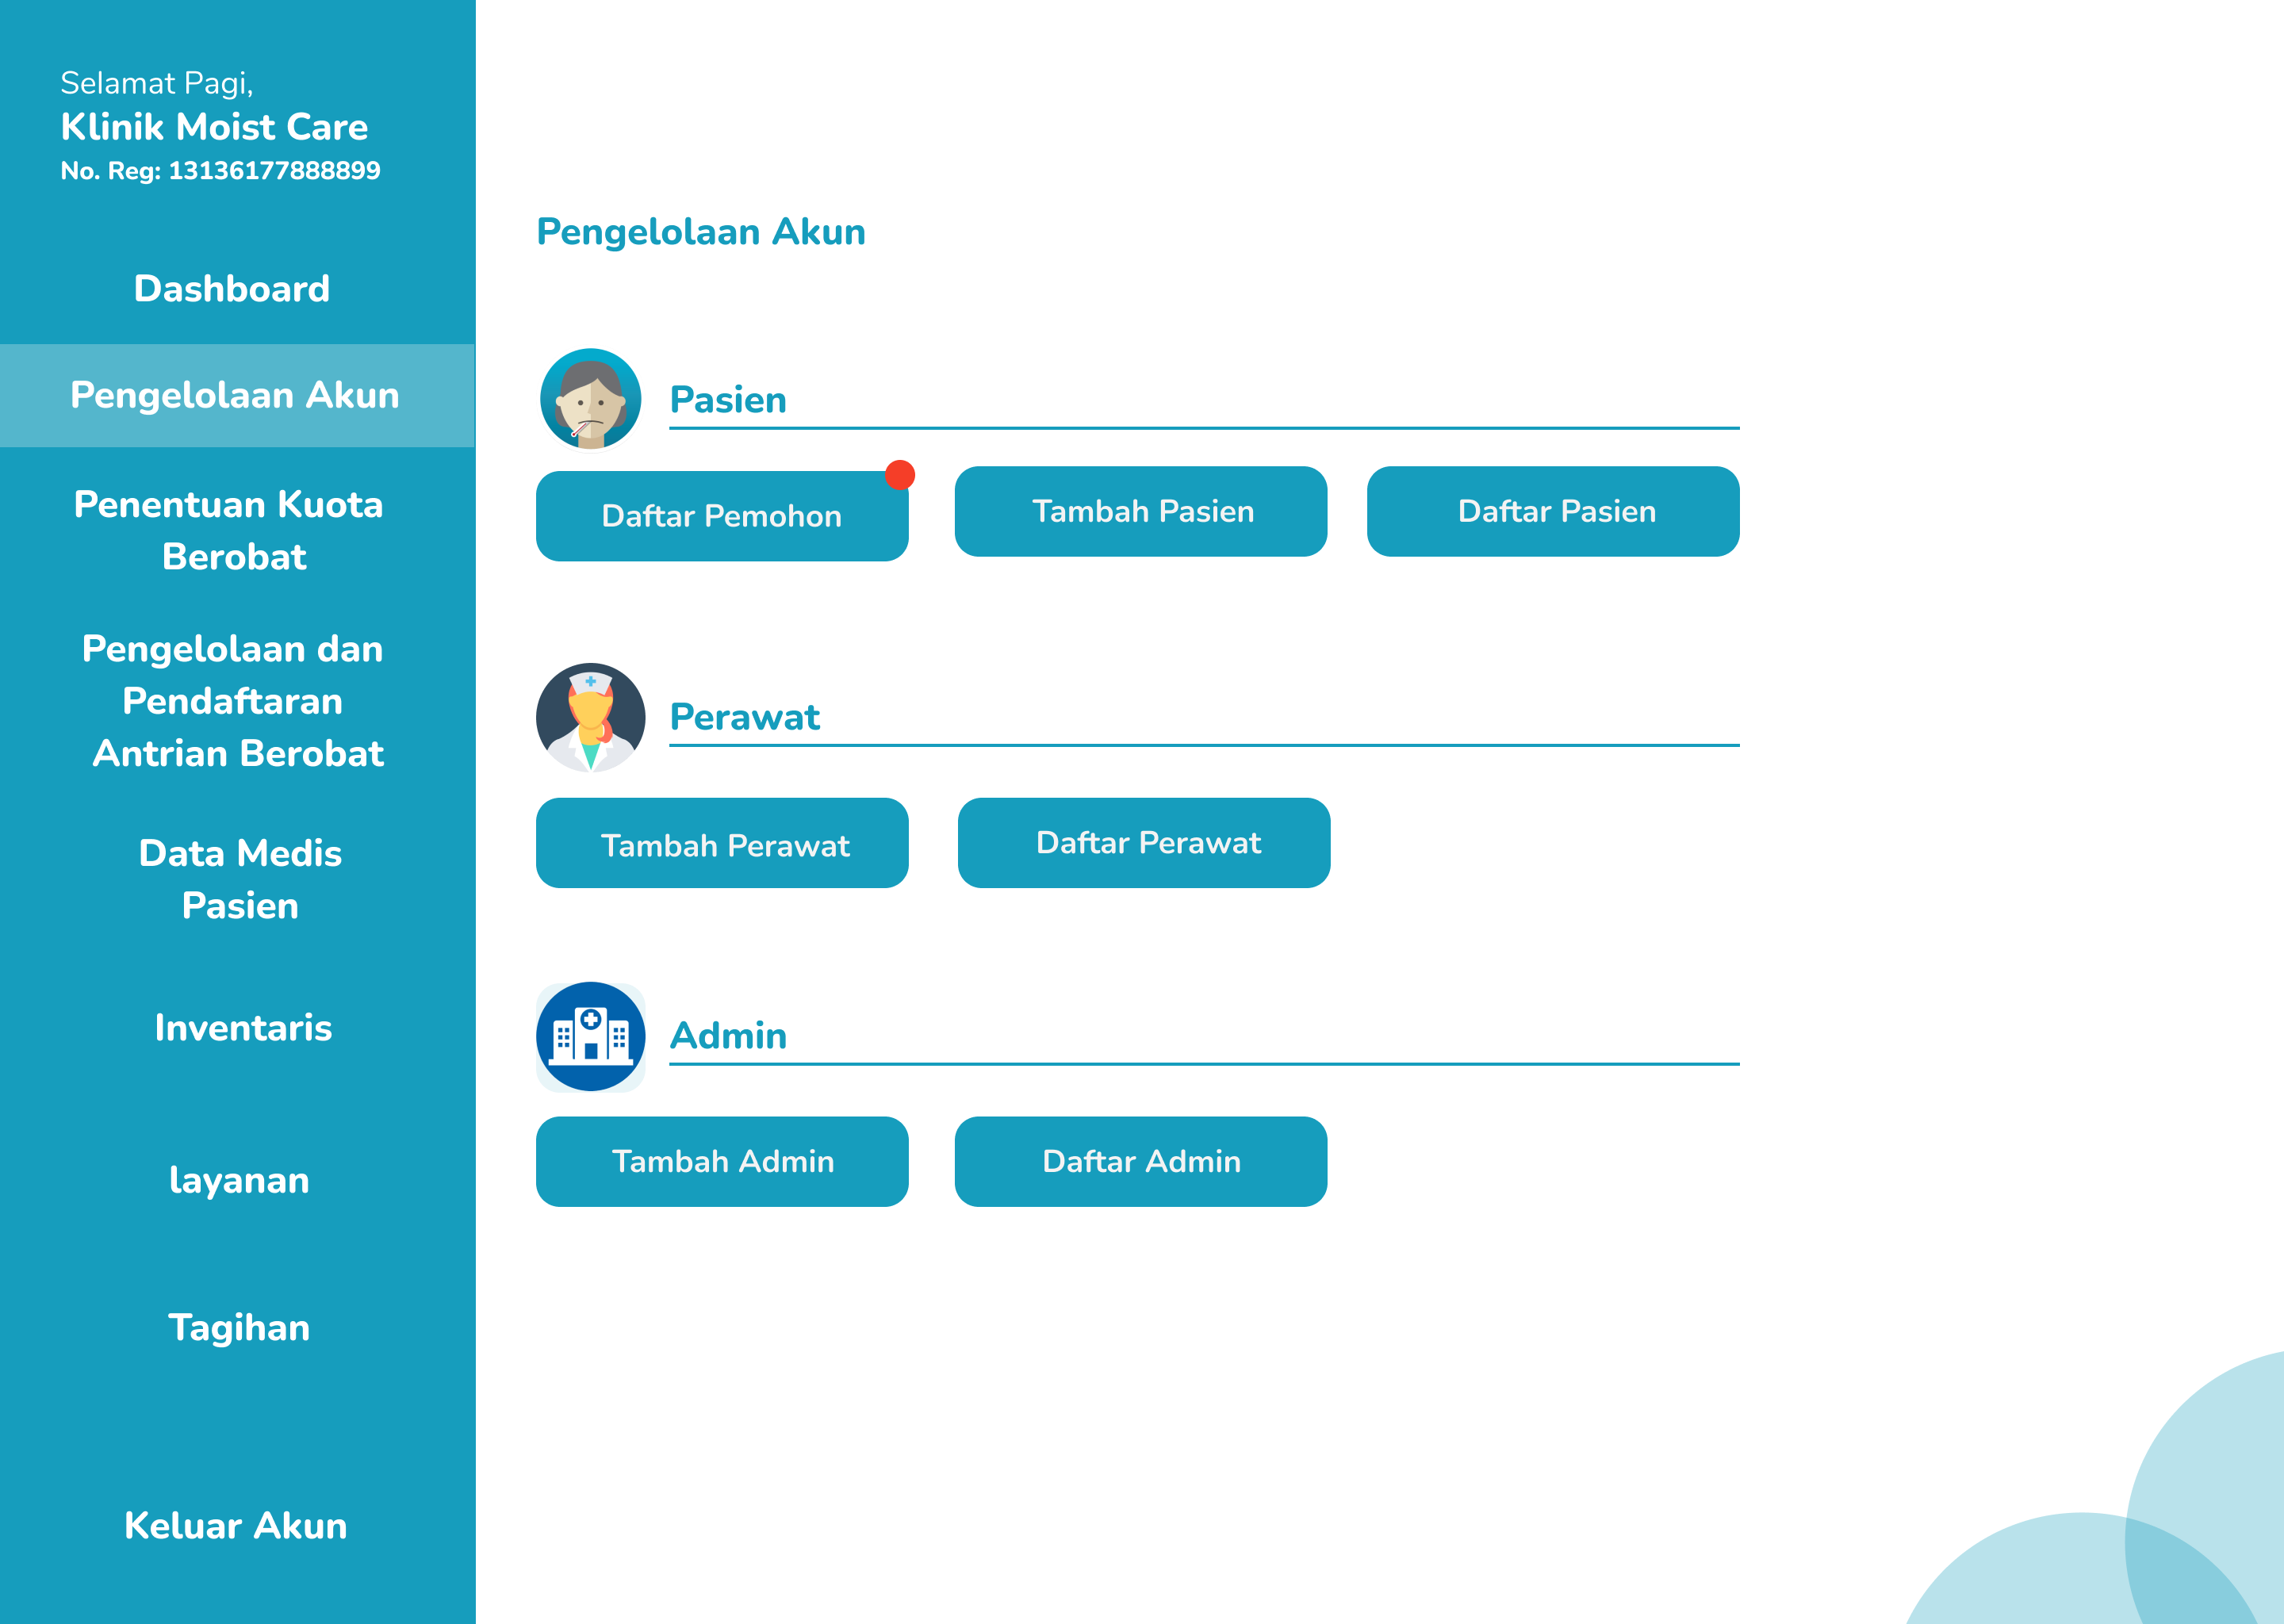
\includegraphics[width=12cm]{gambar/mockup_web/Pembuatan Akun 1.png}
		\caption{\emph{Mock up} tampilan awal pembuatan akun pasien}
		\label{Gambar:tampilanawalpembuatanakunpasien}
	\end{figure}
	
	\textbf{Gambar 4.1} merupakan \emph{mock up} tampilan awal membuat akun pasien. Pada tampilan ini di menu pasien terdapat tombol daftar permohonan pasien untuk melihat \emph{list} akun pasien yang menunggu untuk disetujui pembuatan akunnya. Lalu ada tombol tambah pasien untuk membuat akun pasien baru melalui klinik. Selanjutnya ada tombol daftar pasien untuk melihat semua akun pasien yang terdaftar pada klinik. Di bawah menu pasien ada menu perawat yang berisi tombol tambah perawat untuk membuat akun perawat baru. Lalu tombol daftar perawat untuk melihat semua akun perawat yang terdaftar pada klinik. Selanjutnya di bawah menu perawat ada menu admin yang berisi tombol tambah admin untuk membuat akun admin baru dan ada tombol daftar admin untuk melihat seluruh akun admin yang terdaftar.
	
	Berikutnya saat admin menekan tombol daftar pemohon pada \textbf{Gambar 4.1} maka akan diarahkan ke \textbf{Gambar 4.2}.
	 
	\begin{figure}[H]
		\centering
		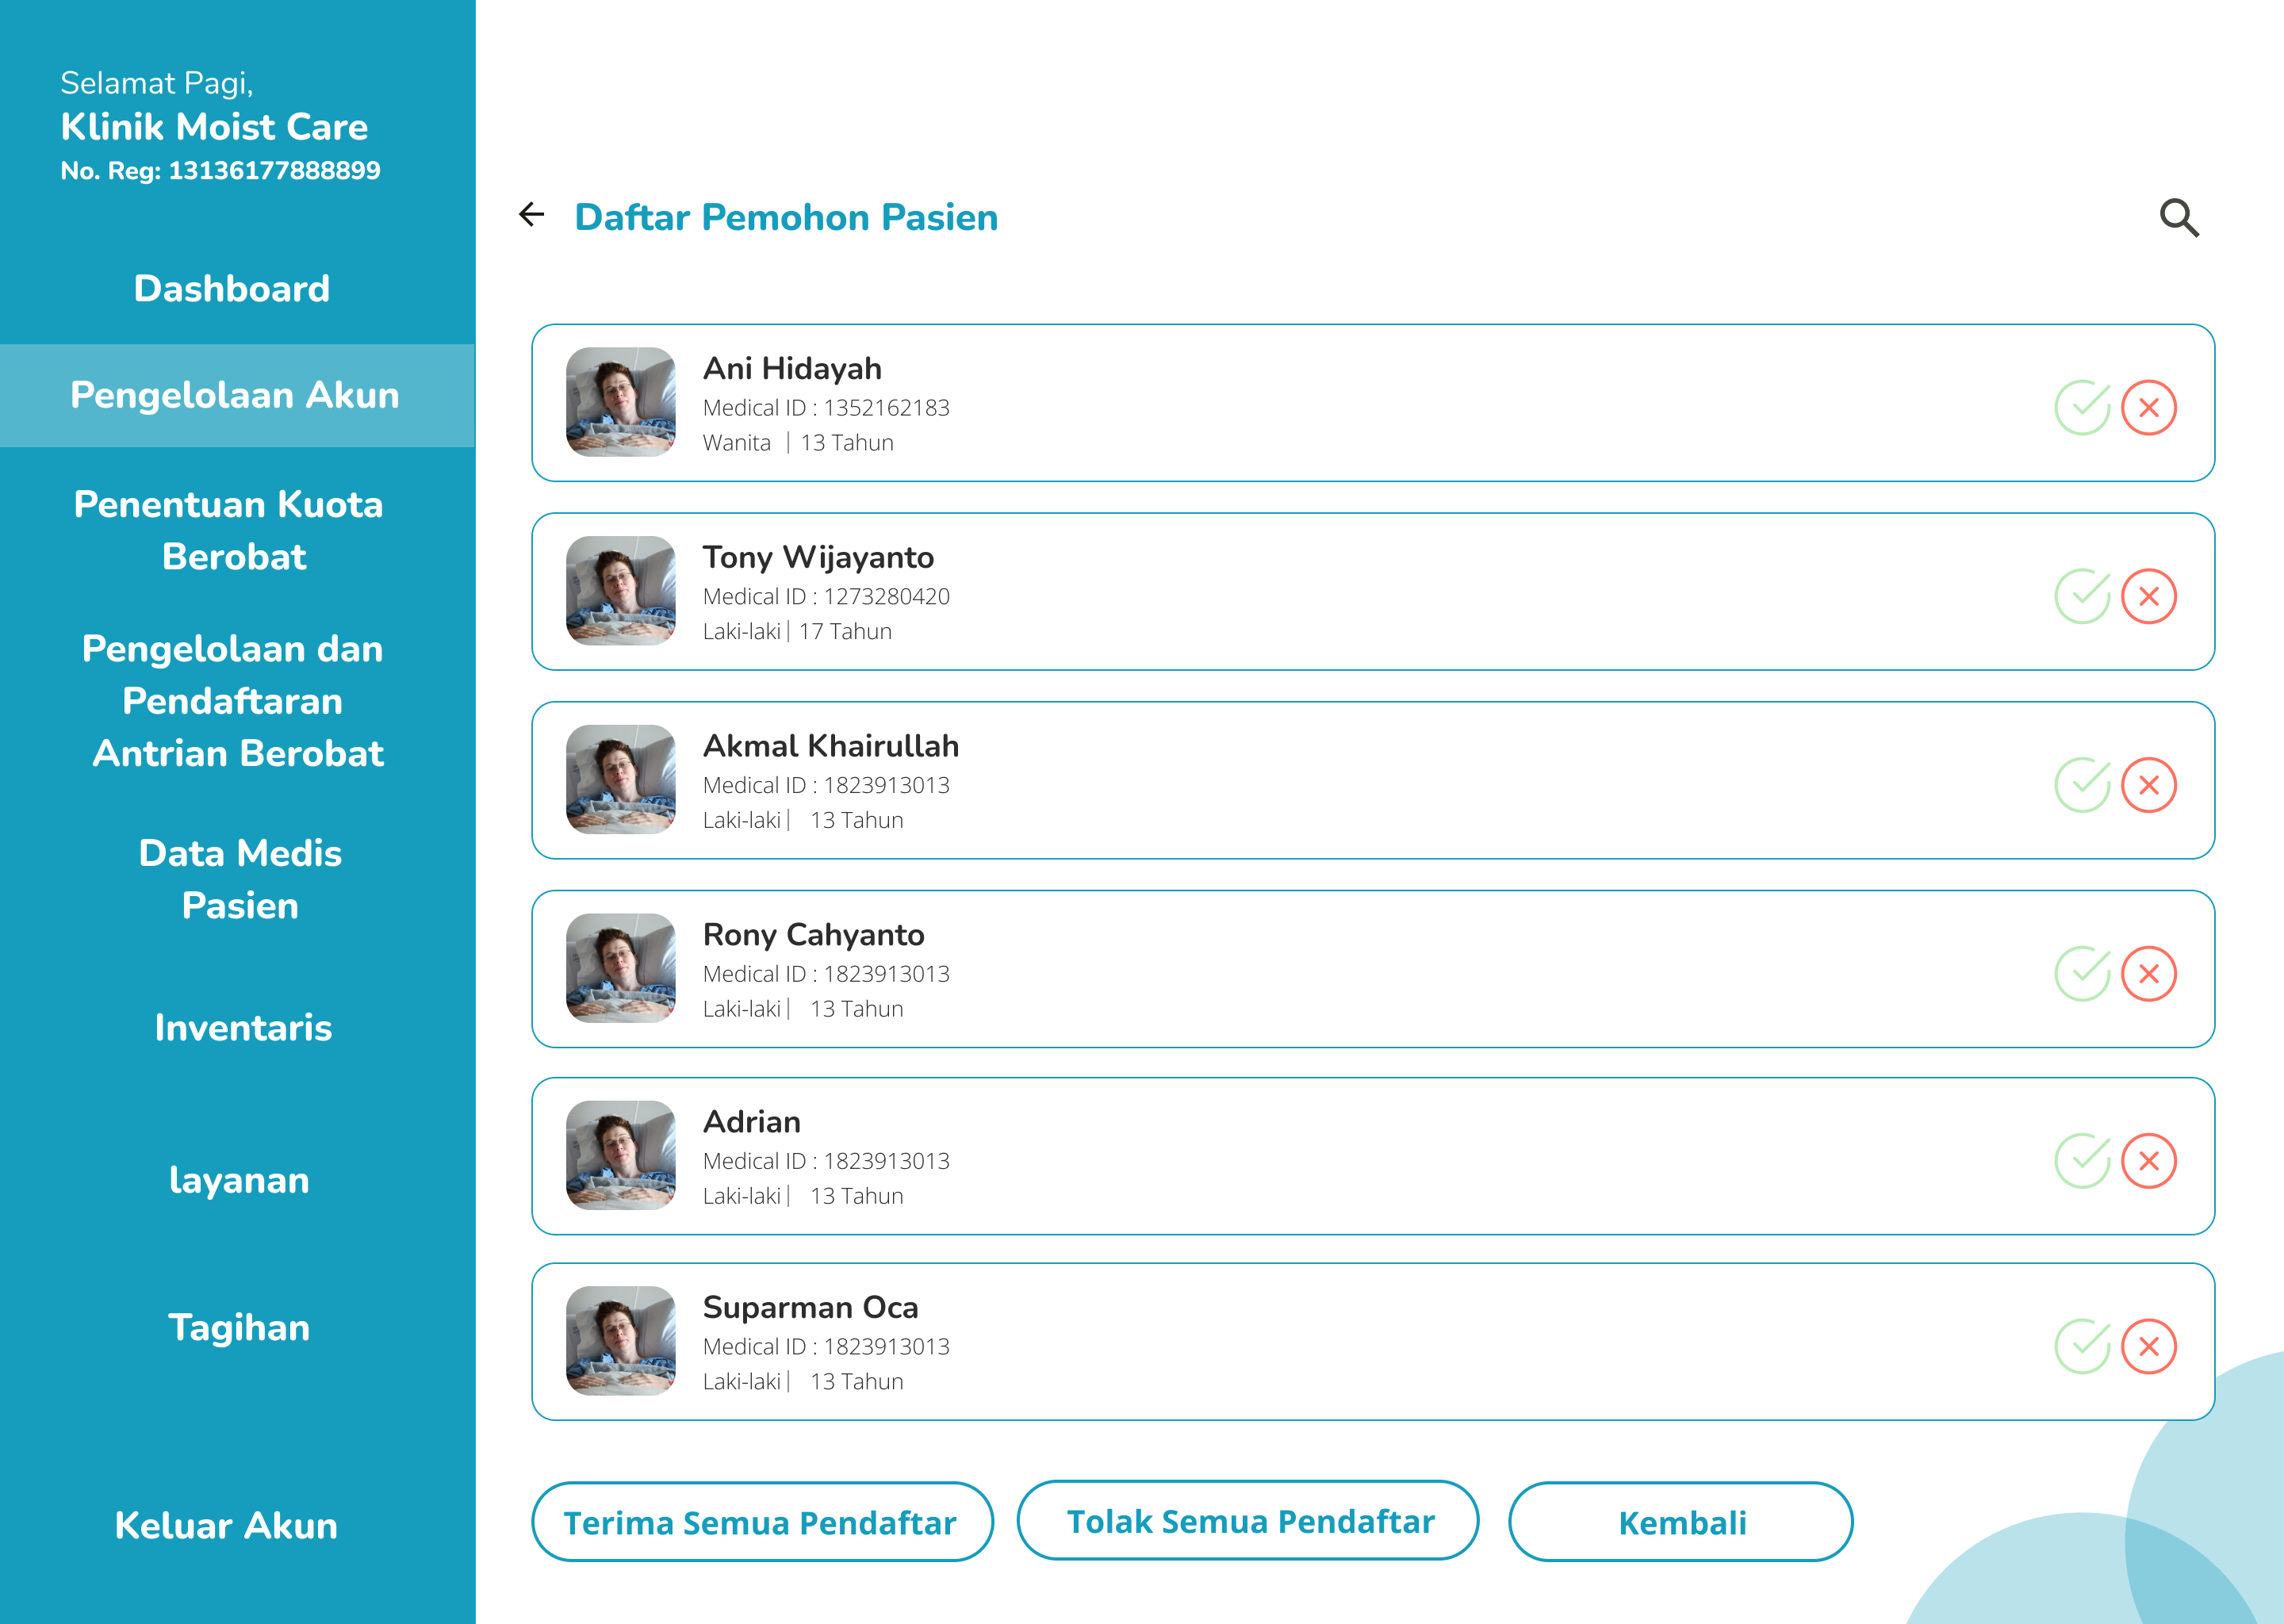
\includegraphics[width=12cm]{gambar/mockup_web/Pembuatan Akun 2.png}
		\caption{\emph{Mock up} tampilan \emph{list} permohonan  pembuatan akun pasien}
		\label{Gambar:listpermohonanpembuatanakunpasien}
	\end{figure}

	\textbf{Gambar 4.2} merupakan tampilan \emph{list} permohonan pembuatan akun pasien. Berisi \emph{list} akun yang menunggu untuk disetujui pembuatan akunnya oleh klinik. Di bawah terdapat tombol terima semua pendaftar untuk menyetujui semua akun yang ada pada \emph{list} permohonan pasien. 	Lalu ada tombol tolak semua pendaftar untuk menolak semua akun yang ada pada \emph{list} permohonan pasien. Dan ada tombol kembali untuk kembali ke tampilan awal pembuatan akun pasien.
	
	Berikutnya ketika admin menekan tombol tambah pasien pada \textbf{Gambar 4.1} maka akan diarahkan ke \textbf{Gambar 4.3}. 
	
	\begin{figure}[H]
		\centering
		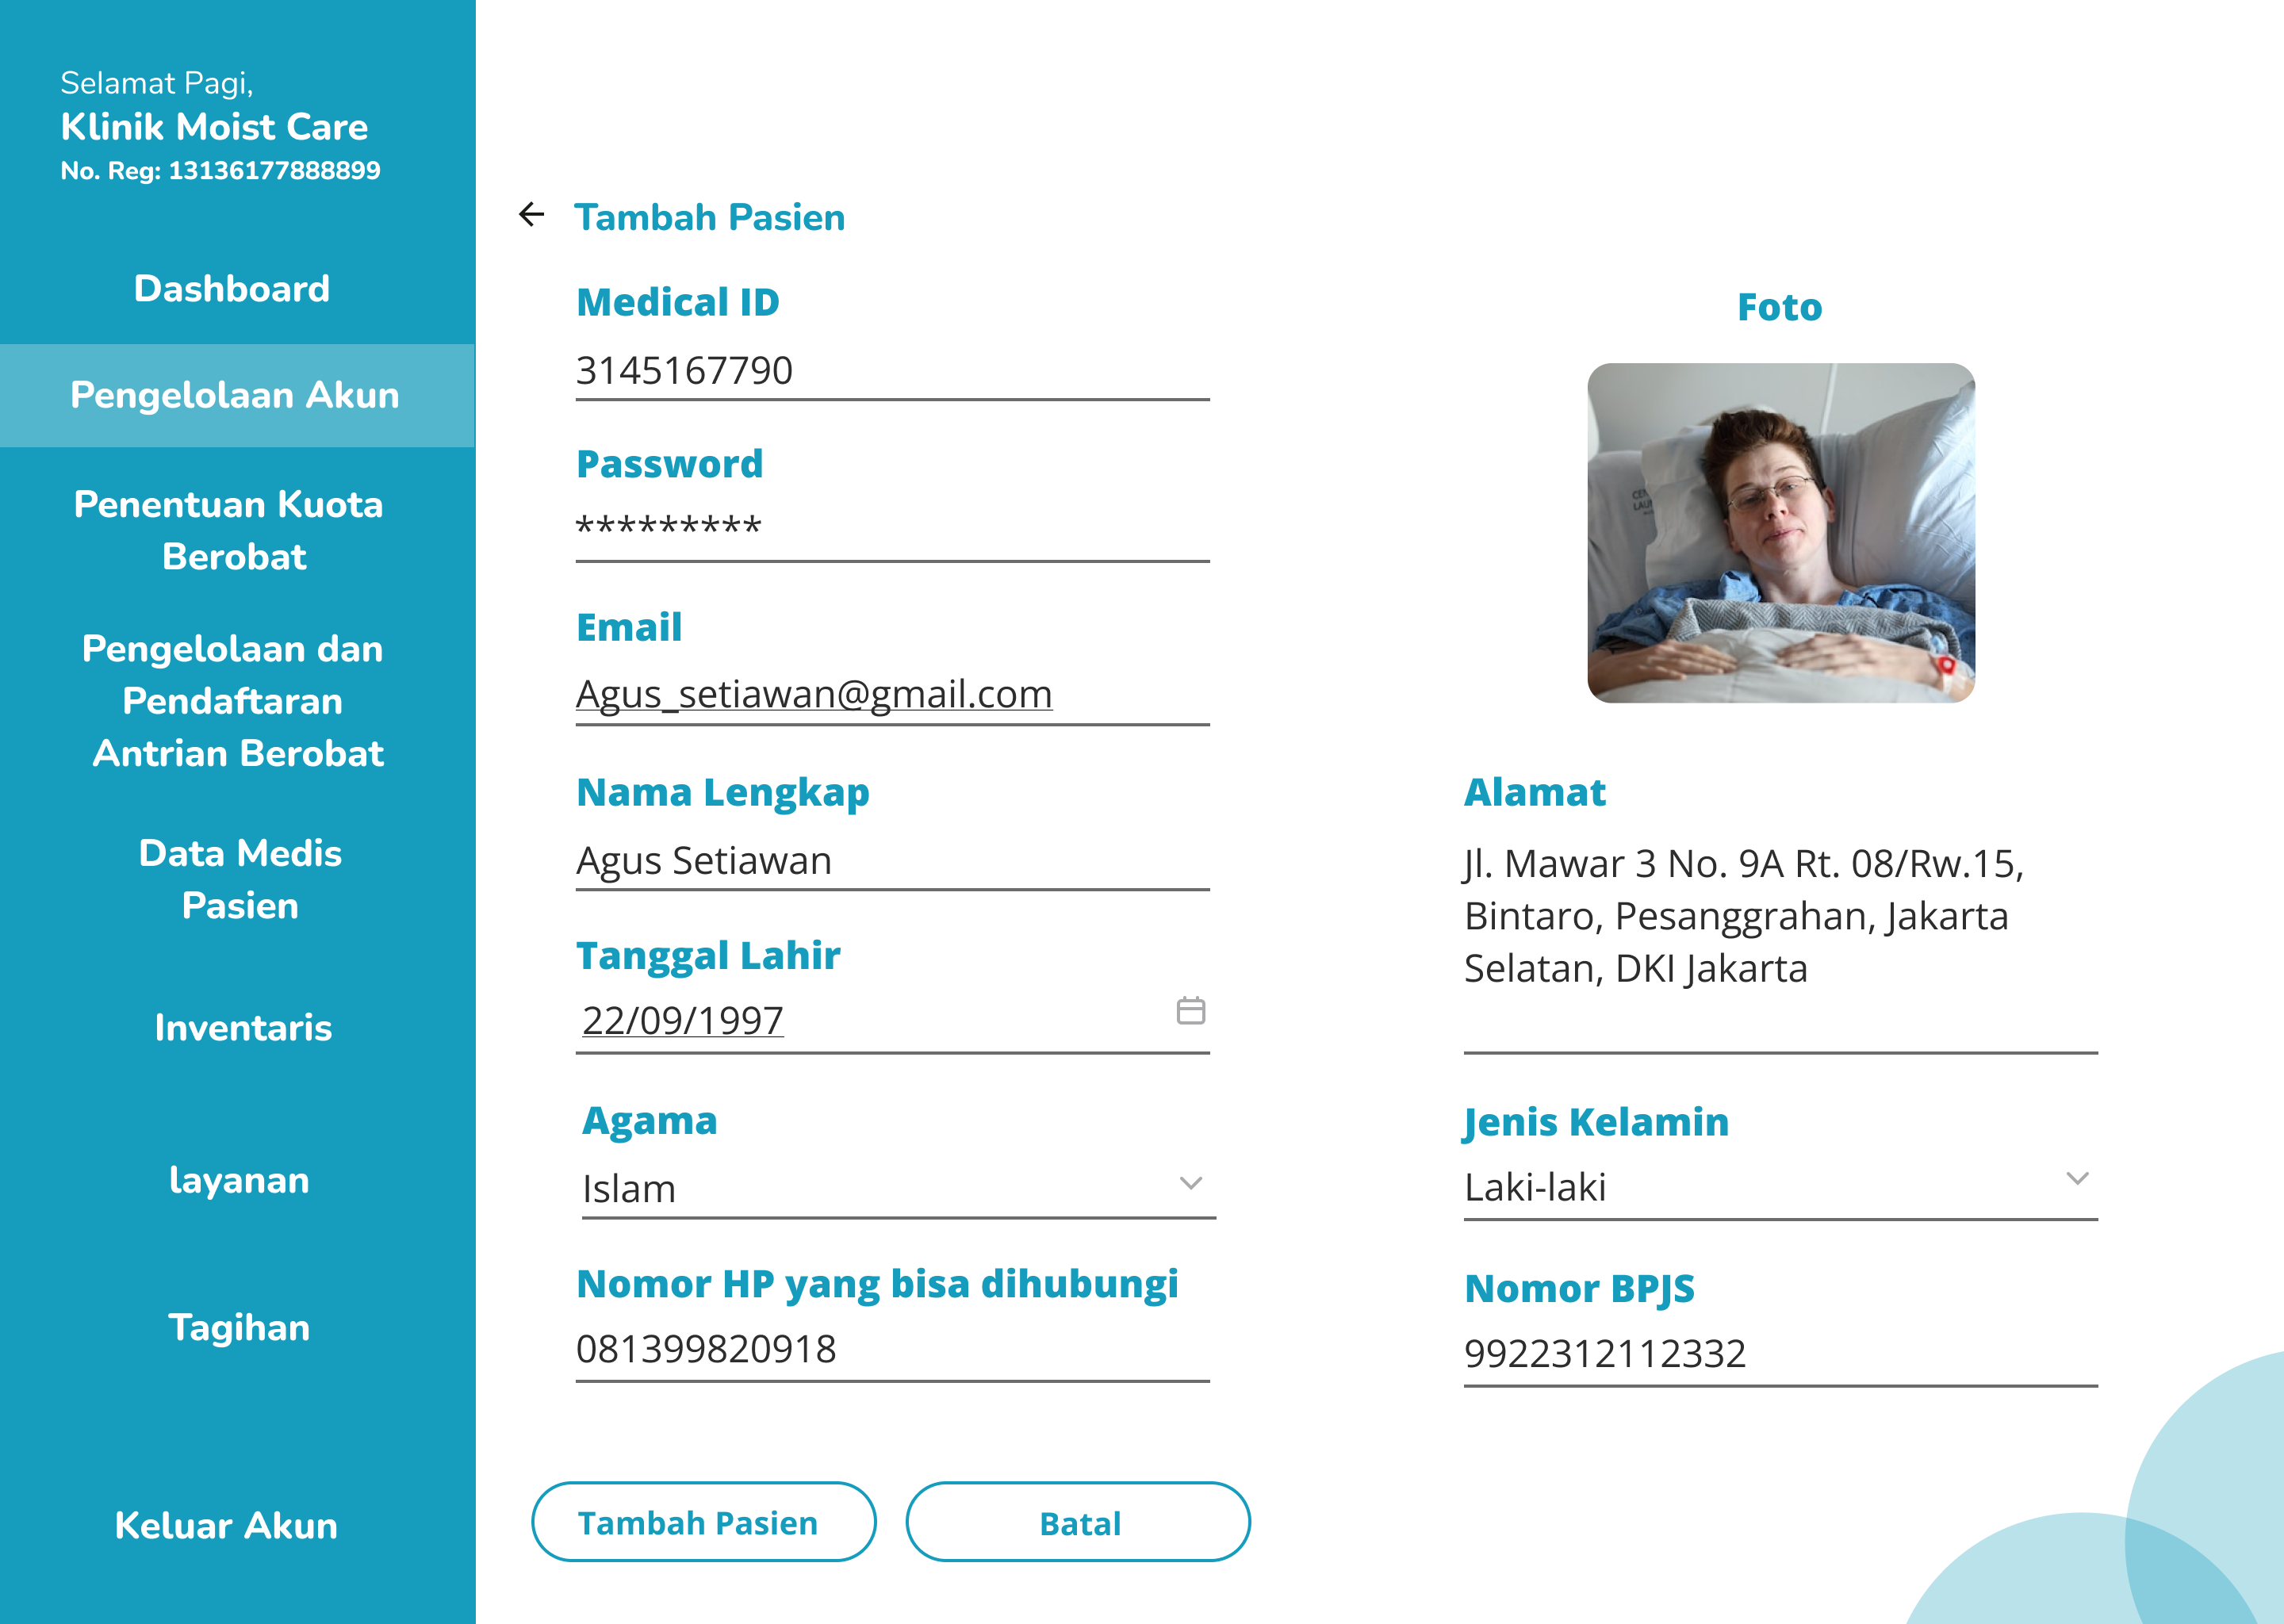
\includegraphics[width=12cm]{gambar/mockup_web/Pembuatan Akun 3.png}
		\caption{\emph{Mock up} pembuatan akun pasien}
		\label{Gambar:pembuatanakunpasien}
	\end{figure}
	
	\textbf{Gambar 4.3} merupakan tampilan pembuatan akun pasien. Saat membuat akun pasien data yang harus diisi adalah medical ID, password, email, nama lengkap, tanggal lahir, agama, Nomor HP yang bisa dihubungi, Nomor BPJS, alamat, foto dan jenis kelamin pasien. Lalu di bawah ada tombol tambah pasien untuk menyimpan akun pasien dan ada tombol batal untuk membatalkan tambah akun pasien yang mengarah kembali ke \textbf{Gambar 4.1}. 
	
	\item Desain \emph{routing table} pembuatan akun pasien
	
	\textbf{Tabel 4.4} pada halaman selanjutnya merupakan \emph{routing table} pembuatan akun pasien:
	
	\begin{table}[H]
		\centering
		\caption{\emph{Routing table} pembuatan akun pasien}
		\label{tabel_input}
		\begin{tabular}{|c|c|c|c|c|c|}
			\hline
			\textbf{\emph{Group}} & \textbf{\emph{Name}} & \textbf{API} & \textbf{HTTP} & \textbf{Keterangan} & \textbf{\emph{Return}} \\
			
			& & \textbf{\emph{Endpoint}} & \textbf{\emph{Verb}} & & \textbf{\emph{Type}} \\
			\hline

			Pasien & 
			\emph{CREATE} &
			\emph{/add\_new\_}
			&
			\emph{POST} &
			menampilkan halaman &
			\emph{view}\\
			
			& 
			&
			\emph{patient}&
			&
			tambah pasien oleh&\\
			
			& 
			&
			&
			&
			klinik&\\
			\hline
			
			& 
			\emph{READ} &
			\emph{/list\_patient}&
			\emph{GET} &
			Menampilkan halaman&
			\emph{view}\\
			
			& 
			&
			&
			&
			seluruh pasien yang &\\
			
			& 
			&
			&
			&
			sudah terverifikasi &\\
			
			& 
			&
			&
			&
			oleh klinik &\\
			\hline
			
			& 
			\emph{READ} &
			\emph{/list\_request}
			&
			\emph{GET} &
			menampilkan halaman &
			\emph{view}\\
			
			& 
			&
			\emph{\_new\_patient}&
			&
			\emph{list} pasien yang &\\
			
			& 
			&
			&
			&
			membuat akun mandiri&\\
			
			
			& 
			&
			&
			&
			dan belum terverifikasi&\\
			
			& 
			&
			&
			&
			oleh klinik&\\
			\hline
			
			Pasien& 
			\emph{READ} &
			\emph{/profil\_pasien}&
			\emph{GET} &
			Menampilkan halaman &
			\emph{view}\\
			
			& 
			&
			\emph{/<\_id>}&
			&
			data pasien&\\
			
			& 
			&
			&
			&
			berdasarkan id pasien&\\
			\hline
			
		\end{tabular}
	\end{table}
	
	\item Membuat \emph{database} pasien
	
	\textbf{Gambar 4.4} pada halaman selanjutnya merupakan tabel pasien yang memuat beberapa atribut yaitu id\_pasien, \emph{password}, id\_staff\_klinik, nama dan agama, tanggal\_lahir, usia, jenis\_kelamin, alamat, no\_hp, email, no\_bpjs, verif, \emph{list\_image\_id}, \emph{created\_at} dan \emph{update\_at} . Data tersebut akan disimpan pada \emph{database} MongoDB dan disimpan dalam format JSON. Tabel atau \emph{collection} pasien akan dibuat bersamaan dengan pemanggilan REST API pembuatan akun pasien.
	
	\begin{figure}[H]
		\centering
		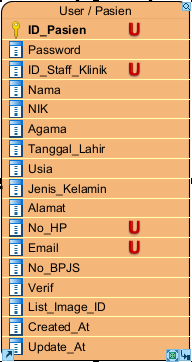
\includegraphics[width=4cm]{gambar/database_pasien.png}
		\caption{Tabel Pasien}
		\label{Gambar:pembuatanakunpasien}
	\end{figure}
	
	\item Pembuatan \emph{mock up} \emph{dashboard} klinik
	
	\begin{figure}[H]
		\centering
		\includegraphics[width=12cm]{gambar/mockup_web/dashboard.png}
		\caption{\emph{Mock up} tampilan awal dashboard klinik}
		\label{Gambar:pengelolaanantrian2}
	\end{figure}
	
	\textbf{Gambar 4.5} merupakan tampilan \emph{dashboard} klinik. Admin dapat melihat statistik kinerja perawat, \emph{cost} perawatan pasien, \emph{income} masuk dan \emph{balance} keuangan dengan detail rata-rata harian, mingguan, dan bulanan.
	
	\item Desain \emph{routing table dashboard} klinik
	
	\textbf{Tabel 4.5} merupakan \emph{routing table} untuk \emph{dashboard} klinik:
	
	\begin{table}[H]
		\centering
		\caption{\emph{Routing table dashboard} klinik}
		\label{tabel_input}
		\begin{tabular}{|c|c|c|c|c|c|}
			\hline
			\textbf{\emph{Group}} & \textbf{\emph{Name}} & \textbf{API} & \textbf{HTTP} & \textbf{Keterangan} & \textbf{\emph{Return}} \\
			
			& & \textbf{\emph{Endpoint}} & \textbf{\emph{Verb}} & & \textbf{\emph{Type}} \\
			\hline
			
			\emph{Dashboard}& 
			\emph{READ} &
			/ &
			\emph{GET} &
			Menampilkan halaman &
			\emph{view}\\
			
			& 
			&
			&
			&
			\emph{dashboard} klinik &
			\\
			\hline
			
		\end{tabular}
	\end{table}
	
	\item Desain \emph{routing table} pemeriksaan kesehatan
	
	\textbf{Tabel 4.6} dan \textbf{Tabel 4.7} merupakan \emph{routing table} untuk pemeriksaan kesehatan:
	
	\begin{table}[H]
		\centering
		\caption{\emph{Routing table} pemeriksaan kesehatan}
		\label{tabel_input}
		\begin{tabular}{|c|c|c|c|c|c|}
			\hline
			\textbf{\emph{Group}} & \textbf{\emph{Name}} & \textbf{API} & \textbf{HTTP} & \textbf{Keterangan} & \textbf{\emph{Return}} \\
			
			& & \textbf{\emph{Endpoint}} & \textbf{\emph{Verb}} & & \textbf{\emph{Type}} \\
			\hline
			
			Pemeri-& 
			\emph{READ} &
			/\emph{list\_patient} &
			\emph{GET} &
			Menampilkan halaman &
			\emph{view}\\
			
			ksaan& 
			&
			\_\emph{medical}&
			&
			\emph{list} pasien yang  &
			\\
			
			Keseha-& 
			&
			\_\emph{check}&
			&
			telah melakukan &
			\\
			
			tan& 
			&
			&
			&
			pemeriksaan kesehatan &
			\\
			\hline
			
			& 
			\emph{READ} &
			/\emph{list\_medical} &
			\emph{GET} &
			Menampilkan halaman &
			\emph{view}\\
			
			& 
			&
			\_\emph{\_check\_}&
			&
			\emph{list} hasil pemeriksaan &
			\\
			
			& 
			&
			\_\emph{data/<nik>}&
			&
			kesehatan 1 pasien &
			\\
			\hline				
			
		\end{tabular}
	\end{table}
	
	\begin{table}[H]
		\centering
		\caption{\emph{Routing table} pemeriksaan kesehatan - lanjutan}
		\label{tabel_input}
		\begin{tabular}{|c|c|c|c|c|c|}
			\hline
			\textbf{\emph{Group}} & \textbf{\emph{Name}} & \textbf{API} & \textbf{HTTP} & \textbf{Keterangan} & \textbf{\emph{Return}} \\
			
			& & \textbf{\emph{Endpoint}} & \textbf{\emph{Verb}} & & \textbf{\emph{Type}} \\
			\hline
			
			Pemeri-& 
			\emph{READ} &
			/detail\_ &
			\emph{GET} &
			Menampilkan halaman &
			\emph{view}\\
			
			ksaan& 
			&
			\_\emph{medical\_}&
			&
			detail hasil pemeriksaan &
			\\
			
			Keseha-& 
			&
			check\_data&
			&
			kesehatan &
			\\
			
			tan& 
			&
			/<\_id>&
			&
			&
			\\
			\hline				
			
		\end{tabular}
	\end{table}
	
	\item Membuat \emph{database} pemeriksaan kesehatan
	
	\begin{figure}[H]
		\centering
		\includegraphics[width=5cm]{gambar/database_data_pemeriksaan_kesehatan.png}
		\caption{Tabel pemeriksaan kesehatan}
		\label{Gambar:pengelolaanantrian2}
	\end{figure}

	\textbf{Gambar 4.6} merupakan tabel pemeriksaan kesehatan memuat beberapa atribut yaitu id\_pk, NIP, tanggal, NIK pasien, tekanan\_darah, nadi, jenis\_kelamin, alamat, no\_hp, email, no\_bpjs, verif, suhu, GDS dan ABPI . Data tersebut akan disimpan pada \emph{database} MongoDB dan disimpan dalam format JSON.
	
	\break
	\item Pembuatan \emph{mock up} proses pengobatan luka
	
	Pada \textbf{Gambar 4.7} pada halaman selanjutnya merupakan tampilan awal data medis pasien. Terdapat \emph{list} data medis pasien beserta tombol lihat. Admin maupun perawat dapat menyeleksi data berdasarkan pasien atau perawat pada \emph{field} dikategorikan berdasarkan perawat. Dan terdapat juga \emph{search bar} untuk mencari data medis pasien berdasarkan kata kunci \emph{Medical} ID atau nomor BPJS.
	
	\begin{figure}[H]
		\centering
		\includegraphics[width=12cm]{gambar/mockup_web/Proses Pengobatan 1.png}
		\caption{\emph{Mock up} tampilan awal data medis pasien}
		\label{Gambar:pengelolaanantrian2}
	\end{figure}
	
	Ketika admin menekan tombol lihat pada data pasien yang dipilih pada \textbf{Gambar 4.7} maka akan diarahkan ke \textbf{Gambar 4.8} pada halaman selanjutnya yang merupakan profil data medis pasien dan berisikan data berupa \emph{Medical} ID, email, nama lengkap, tanggal lahir, agama, nomor hp, alamat, jenis kelamin, foto, dan nomor BPJS. Selanjutnya terdapat tombol profil, histori kajian dan galeri luka. Dan terdapat tombol kembali untuk menuju ke halaman sebelumnya.
	
	\begin{figure}[H]
		\centering
		\includegraphics[width=12cm]{gambar/mockup_web/Proses Pengobatan 2.png}
		\caption{\emph{Mock up} profil data medis pasien}
		\label{Gambar:pengelolaanantrian2}
	\end{figure}
	
	Ketika admin menekan tombol histori kajian pada \textbf{Gambar 4.8} maka akan diarahkan ke \textbf{Gambar 4.9}. 
	
	\begin{figure}[H]
		\centering
		\includegraphics[width=12cm]{gambar/mockup_web/Proses Pengobatan 3.png}
		\caption{\emph{Mock up list} histori kajian data medis pasien}
		\label{Gambar:pengelolaanantrian2}
	\end{figure}
	
	\textbf{Gambar 4.9} merupakan histori kajian data medis pasien berisi \emph{list} kajian yang telah dilaksanakan dan diurutkan berdasarkan tanggal dengan detail data nama dan nip perawat yang melakukan kajian beserta tombol lihat. Dan terdapat tombol kembali untuk menuju ke halaman sebelumnya.
	
	Ketika admin menekan tombol lihat pada salah satu histori kajian pada \textbf{Gambar 4.9} maka akan diarahkan ke \textbf{Gambar 4.10} yang merupakan detail histori kajian data medis pasien berisi foto luka yang diambil saat kajian berlangsung dan skoring kajian luka pasien. Dan terdapat tombol kembali untuk kembali ke halaman sebelumnya.
	
	\begin{figure}[H]
		\centering
		\includegraphics[width=12cm]{gambar/mockup_web/Proses Pengobatan 4.png}
		\caption{\emph{Mock up} detail histori kajian data medis pasien}
		\label{Gambar:pengelolaanantrian2}
	\end{figure}
	
	Ketika admin menekan tombol galeri luka \textbf{Gambar 4.8} maka akan diarahkan ke \textbf{Gambar 4.11} pada halaman selanjutnya yang merupakan galeri luka pasien dari semua histori kajian. Dan terdapat tombol kembali untuk menuju halaman sebelumnya.
	
	\begin{figure}[H]
		\centering
		\includegraphics[width=12cm]{gambar/mockup_web/Proses Pengobatan 5.png}
		\caption{\emph{Mock up} galeri luka pasien}
		\label{Gambar:pengelolaanantrian2}
	\end{figure}
	
	\begin{figure}[H]
		\centering
		\includegraphics[width=12cm]{gambar/mockup_web/Inventaris1.png}
		\caption{\emph{Mock up} tampilan awal inventaris}
		\label{Gambar:pengelolaanantrian2}
	\end{figure}
	
	\textbf{Gambar 4.12} merupakan tampilan awal inventaris didalamnya terdapat \emph{list} barang berupa obat, balutan, dan komponen lainnya beserta detail stok, harganya dan tombol \emph{edit}. Terdapat juga tombol semua barang, obat, balutan, lainnya dan tambah obat/komponen.
	
	\begin{figure}[H]
		\centering
		\includegraphics[width=12cm]{gambar/mockup_web/Layanan1.png}
		\caption{\emph{Mock up} tampilan awal layanan}
		\label{Gambar:pengelolaanantrian2}
	\end{figure}
	
	\textbf{Gambar 4.13} merupakan tampilan awal layanan didalamnya terdapat \emph{list} layanan beserta detail keterangana layanan, harganya dan tombol \emph{edit}.
	
	\break
	\item Desain \emph{routing table} proses pengobatan
	
	\textbf{Tabel 4.8}, \textbf{Tabel 4.9} dan \textbf{Tabel 4.10} merupakan \emph{routing table} untuk proses pengobatan:
	
	\begin{table}[H]
		\centering
		\caption{\emph{Routing table} proses pengobatan}
		\label{tabel_input}
		\begin{tabular}{|c|c|c|c|c|c|}
			\hline
			\textbf{\emph{Group}} & \textbf{\emph{Name}} & \textbf{API} & \textbf{HTTP} & \textbf{Keterangan} & \textbf{\emph{Return}} \\
			
			& & \textbf{\emph{Endpoint}} & \textbf{\emph{Verb}} & & \textbf{\emph{Type}} \\
			\hline
			
			Pengo- & 
			\emph{READ} &
			/data\_kajians&
			\emph{GET} &
			Menampilkan halaman &
			\emph{view}\\
			
			
			batan& 
			&
			&
			&
			data kajian semua &\\
			
			& 
			&
			&
			&
			pasien berdasarkan nama &\\
			
			& 
			&
			&
			&
			pasien &\\
			\hline
			
			& 
			\emph{READ} &
			/data\_kajians&
			\emph{GET} &
			Menampilkan data &
			\{<nip>,\\
			
			
			& 
			&
			/<nip>&
			&
			kajian semua pasien &
			<nama\_\\
			
			& 
			&
			&
			&
			berdasarkan nama &
			pegawai>,\\
			
			& 
			&
			&
			&
			perawat &
			<nrm>,\\
			
			& 
			&
			&
			&
			&
			<nama\_\\
			
			& 
			&
			&
			&
			&
			pasien>\}\\
			\hline
			
			& 
			\emph{READ} &
			/data\_kajians&
			\emph{GET} &
			Menampilkan data &
			\{<nrm>,\\
			
			
			& 
			&
			/<nrm>&
			&
			kajian semua pasien&
			<nama\_\\
			
			& 
			&
			&
			&
			berdasarkan nomor &
			pasien>\}\\
			
			& 
			&
			&
			&
			rekam medis &
			\\
			\hline
			
			& 
			\emph{READ} &
			/profil\_&
			\emph{GET} &
			Menampilkan halaman &
			\emph{view}\\
			
			
			& 
			&
			pasien&
			&
			profil 1 pasien &
			\\
			
			& 
			&
			/<nrm>&
			&
			berdasarkan NRM &
			\\
			\hline
			
		\end{tabular}
	\end{table}
	
	\begin{table}[H]
		\centering
		\caption{\emph{Routing table} proses pengobatan - lanjutan 1}
		\label{tabel_input}
		\begin{tabular}{|c|c|c|c|c|c|}
			\hline
			\textbf{\emph{Group}} & \textbf{\emph{Name}} & \textbf{API} & \textbf{HTTP} & \textbf{Keterangan} & \textbf{\emph{Return}} \\
			
			& & \textbf{\emph{Endpoint}} & \textbf{\emph{Verb}} & & \textbf{\emph{Type}} \\
			\hline
			
			Pengo-& 
			\emph{READ} &
			/\emph{list}\_data&
			\emph{GET} &
			Menampilkan &
			\emph{view}\\
			
			
			batan& 
			&
			\_kajian&
			&
			halaman \emph{list} histori&
			\\
			
			& 
			&
			/<nrm>&
			&
			 kajian 1 pasien&
			\\
			
			& 
			&
			&
			&
			berdasarkan NRM  &
			\\
			\hline
			
			& 
			\emph{READ} &
			/galeri\_luka&
			\emph{GET} &
			Menampilkan  &
			\emph{view}\\
			
			
			& 
			&
			/<nrm>&
			&
			halaman galeri luka  &
			\\
			
			& 
			&
			&
			&
			pasien berdasarkan&
			\\
			
			& 
			&
			&
			&
			NRM&
			\\
		
			\hline
			
			Inven& 
			\emph{READ} &
			/\emph{list}\_&
			\emph{GET} &
			Menampilkan&
			\emph{view}\\
			
			
			-taris& 
			&
			inventaris&
			&
			halaman \emph{list}&
			\\
			
			& 
			&
			&
			&
			semua inventaris&
			\\
			\hline
			
			& 
			\emph{CREATE} &
			/\emph{add}\_&
			\emph{POST} &
			Menampilkan &
			\emph{view}\\
			
			& 
			&
			inventaris&
			&
			halaman tambah&
			\\
			
			& 
			&
			&
			&
			inventaris&
			\\
			\hline
			
			& 
			\emph{UPDATE} &
			/\emph{edit}\_&
			\emph{POST} &
			Menampilkan &
			\emph{view}\\
			
			& 
			&
			inventaris&
			&
			halaman \emph{edit} &
			\\
			
			& 
			&
			/<\_id>&
			&
			inventaris &
			\\
			\hline
			
			& 
			\emph{DESTROY} &
			/\emph{delete}\_&
			\emph{DELETE} &
			Hapus data &
			\emph{view}\\
			
			& 
			&
			inventaris&
			&
			inventaris &
			\\
			
			& 
			&
			/<\_id>&
			&
			&
			\\
			
			\hline
			
			Laya & 
			\emph{READ} &
			/\emph{list}\_ &
			\emph{GET} &
			Menampilkan &
			\emph{view}\\
			
			-nan& 
			&
			layanan&
			&
			halaman \emph{list} &
			\\
			
			& 
			&
			&
			&
			semua layanan &
			\\
			\hline
			
		\end{tabular}
	\end{table}
	
	\begin{table}[H]
		\centering
		\caption{\emph{Routing table} proses pengobatan - lanjutan 2}
		\label{tabel_input}
		\begin{tabular}{|c|c|c|c|c|c|}
			\hline
			\textbf{\emph{Group}} & \textbf{\emph{Name}} & \textbf{API} & \textbf{HTTP} & \textbf{Keterangan} & \textbf{\emph{Return}} \\
			
			& & \textbf{\emph{Endpoint}} & \textbf{\emph{Verb}} & & \textbf{\emph{Type}} \\
			\hline
	
			Laya-& 
			\emph{CREATE} &
			/\emph{add}\_&
			\emph{POST} &
			Menampilkan&
			\emph{view}\\
			
			nan& 
			&
			layanan&
			&
			halaman tambah&
			\\
			
			& 
			&
			&
			&
			layanan&
			\\
			\hline
			
			& 
			\emph{UPDATE} &
			/\emph{edit}&
			\emph{POST} &
			Menampilkan&
			\emph{view}\\
			
			& 
			&
			\_layanan&
			&
			halaman \emph{edit}&
			\\
			
			& 
			&
			/<\_id>&
			&
			layanan&
			\\
			\hline
			
			& 
			\emph{DESTROY} &
			/\emph{delete}&
			\emph{DELETE} &
			Hapus&
			\emph{view}\\
			
			& 
			&
			\_layanan&
			&
			layanan &
			\\
			
			& 
			&
			<\_id>&
			&
			&
			\\
			\hline
			
		\end{tabular}
	\end{table}
	
	\item Membuat \emph{database} proses pengobatan
	
	\begin{figure}[H]
		\centering
		\includegraphics[width=4cm]{gambar/data_kajian_database.png}
		\caption{Tabel data kajian}
		\label{Gambar:pengelolaanantrian2}
	\end{figure}

	\textbf{Gambar 4.14} merupaka data kajian memuat beberapa atribut yaitu id\_kajian, \emph{size}, \emph{edges}, \emph{necrotic\_type}, \emph{necrotic\_amount}, \emph{skincolor\_surround}, \emph{granulation\_tissue}, \emph{epithelization}, raw\_\emph{photo}\_id, tipe\_\emph{image}\_id, diameter\_\emph{image}, dan \emph{created\_at}. Data tersebut akan disimpan pada \emph{database} MongoDB dan disimpan dalam format JSON.
	
	\begin{figure}[H]
		\centering
		\includegraphics[width=4cm]{gambar/inventaris_database.png}
		\caption{Tabel inventaris}
		\label{Gambar:pengelolaanantrian2}
	\end{figure}

	\textbf{Gambar 4.15} merupakan tabel inventaris memuat beberapa atribut yaitu id\_inventaris, id\_\emph{image}, tipe\_inventaris, nama\_inventaris, jumlah, harga, dan keterangan. Data tersebut akan disimpan pada \emph{database} MongoDB dan disimpan dalam format JSON.

	\begin{figure}[H]
		\centering
		\includegraphics[width=4cm]{gambar/layanan_database.png}
		\caption{Tabel layanan}
		\label{Gambar:pengelolaanantrian2}
	\end{figure}
	
	\textbf{Gambar 4.16} merupakan tabel layanan memuat beberapa atribut yaitu id\_layanan, id\_\emph{image}, tipe\_layanan, nama\_layanan, keterangan, dan harga. Data tersebut akan disimpan pada \emph{database} MongoDB dan disimpan dalam format JSON.
	
	\item Pembuatan \emph{mock up} pendaftaran pasien berobat
	
	Pada \textbf{Gambar 4.17} di halaman selanjutnya merupakan tampilan \emph{live} yang berisi  antrian berobat lengkap beserta nama pasien dan nomor antrian.
	
	\begin{figure}[H]
		\centering
		\includegraphics[width=12cm]{gambar/mockup_web/Pendaftaran Akun Berobat.png}
		\caption{\emph{Mock up} melihat daftar dan urutan pasien yang akan dilayani}
		\label{Gambar:pendaftaranakunberobat1}
	\end{figure}
	
	\item Desain \emph{routing table} pendaftaran pasien berobat. 
	
	\textbf{Tabel 4.11} merupakan \emph{routing table} untuk pendaftaran pasien berobat:
	
	\begin{table}[H]
		\centering
		\caption{\emph{Routing table} pendaftaran pasien berobat}
		\label{tabel_input}
		\begin{tabular}{|c|c|c|c|c|c|}
			\hline
			\textbf{\emph{Group}} & \textbf{\emph{Name}} & \textbf{API} & \textbf{HTTP} & \textbf{Keterangan} & \textbf{\emph{Return}} \\
			
			& & \textbf{\emph{Endpoint}} & \textbf{\emph{Verb}} & & \textbf{\emph{Type}} \\
			\hline
			
			& 
			\emph{READ} &
			/antrian&
			\emph{GET} &
			Menampilkan halaman&
			\emph{view}\\
			
			
			& 
			&
			\emph{\_real\_time}&
			&
			daftar dan urutan pasien&\\
			
			& 
			&
			&
			&
			yang akan dilayani &\\
			\hline
			
		\end{tabular}
	\end{table}
	
	\item Membuat \emph{database} pendaftaran pasien berobat
	
	\textbf{Gambar 4.18} pada halaman selanjutnya merupakan tabel detail tagihan memuat beberapa atribut yaitu id\_pendaftaran, tipe\_pendaftaran, id\_pasien dan \emph{created\_at}. Data tersebut akan disimpan pada \emph{database} MongoDB dan disimpan dalam format JSON.
	
	\begin{figure}[H]
		\centering
		\includegraphics[width=6cm]{gambar/Pendaftaran_database.png}
		\caption{Tabel pendaftaran berobat}
		\label{Gambar:pengelolaanantrian1}
	\end{figure}
	
	\item Pembuatan \emph{mock up} pengelolaan antrian
	
	\textbf{Gambar 4.19} merupakan tampilan menentukan kuota pelayanan pasien yang mendaftar secara \emph{offline} maupun \emph{online} pada hari yang ditentukan.
	
	\begin{figure}[H]
		\centering
		\includegraphics[width=12cm]{gambar/mockup_web/Pengelolaan Antrian Akun 1.png}
		\caption{\emph{Mock up} menentukan kuota pelayanan pasien yang mendaftar secara \emph{offline} maupun \emph{online} pada hari yang ditentukan}
		\label{Gambar:pengelolaanantrian1}
	\end{figure}
	
	Pada halaman ini admin harus memilih dan mengisi tanggal berobat beserta kuota pasien yang daftar berobat secara \emph{online} dan kuota pasien yang mendaftar secara \emph{offline} atau daftar langsung di klinik. Dan terdapat tombol simpan untuk menyimpan data kuota berobat pada hari yang ditentukan yang telah diisi.
	
	\textbf{Gambar 4.20} merupakan tampilan awal melakukan pendaftaran pasien yang akan berobat secara \emph{offline} maupun \emph{online}. Terdapat \emph{fields} memilih tanggal untuk mengambil data kuota berobat pada hari yang ditentukan yang telah di-\emph{set} sebelumnya. Lalu terdapat \emph{list} antrian pasien berobat yang sudah dikonfirmasi pendaftarannya beserta tombol ceklis untuk memvalidasi bahwa pasien sudah mendapatkan pelayanan berobat klinik dan tombol silang untuk membatalkan pasien yang sudah dikonfirmasi pendaftarannnya apabila pasien tidak jadi berobat. 
	
	\begin{figure}[H]
		\centering
		\includegraphics[width=12cm]{gambar/mockup_web/Pengelolaan Antrian Akun 2.png}
		\caption{\emph{Mock up} tampilan awal melakukan pendaftaran pasien yang akan berobat secara \emph{offline} maupun \emph{online}}
		\label{Gambar:pendaftaranakunberobat}
	\end{figure}

	Selanjutnya terdapat tombol pendaftar \emph{online} untuk melihat \emph{list} pasien yang sudah mendaftar berobat secara \emph{online} namun belum dikonfirmasi. Terdapat juga tombol tambah \emph{offline} untuk tambah pasien berobat secara manual apabila pasien daftar secara \emph{offline} atau langsung. lalu tombol \emph{plus icon} untuk memajukan antrian dan tombol \emph{minus icon} untuk memundurkan antrian. Selanjutnya tombol \emph{reset} antrian untuk me-\emph{reset} antrian kembali ke nomor 1. Dan tombol tampilkan \emph{2nd display} antrian berobat untuk tampilan tv \emph{live} di ruang tunggu pasien.
	
	Ketika admin menekan tombol tambah pasien \emph{offline} pada \textbf{Gambar 4.20} pada halaman sebelumnya maka muncul \emph{list} daftar pasien pada \textbf{Gambar 4.21} beserta tombol tambah untuk meng-\emph{input} pasien ke dalam antrian berobat dan admin bisa mencari pasien yang ingin daftar berobat dengan mencari lewat \emph{Medical} ID atau nomor BPJS. Dan ada tombol kembali untuk kembali ke tampilan \textbf{Gambar 4.15}
	
	\begin{figure}[H]
		\centering
		\includegraphics[width=12cm]{gambar/mockup_web/Pengelolaan Antrian Akun 3.png}
		\caption{\emph{Mock up} mendaftarkan pasien yang berobat secara \emph{offline}}
		\label{Gambar:pengelolaanantrian2}
	\end{figure}
	
	\item Desain \emph{routing table} pengelolaan antrian. 
	
	\textbf{Tabel 4.12} pada halaman selanjutnya merupakan \emph{routing table} untuk pengelolaan antrian:
	
	\begin{table}[H]
		\centering
		\caption{\emph{Routing table} pengelolaan antrian - lanjutan}
		\label{tabel_input}
		\begin{tabular}{|c|c|c|c|c|c|}
			\hline
			\textbf{\emph{Group}} & \textbf{\emph{Name}} & \textbf{API} & \textbf{HTTP} & \textbf{Keterangan} & \textbf{\emph{Return}} \\
			
			& & \textbf{\emph{Endpoint}} & \textbf{\emph{Verb}} & & \textbf{\emph{Type}} \\
			\hline
			
			Antrian & 
			\emph{CREATE} &
			/kuota &
			\emph{POST} &
			Menampilkan halaman &
			\emph{view}\\
			
			& 
			&
			&
			&
			menentukan kuota &\\
			
			& 
			&
			&
			&
			jumlah pasien berobat&\\
			\hline
			
			& 
			\emph{READ}&
			/antrian &
			\emph{GET}&
			menampilkan halaman &
			\emph{view}\\
			
			& 
			&
			&
			&
			antrian pasien berobat&\\
			\hline
			
			& 
			\emph{UPDATE}&
			/\emph{list}\_daftar&
			\emph{POST}&
			Menampilkan halaman &
			\emph{view}\\
			
			
			& 
			&
			\_berobat&
			&
			\emph{list} pasien yang telah &\\
			
			& 
			&
			\_\emph{online}&
			&
			daftar berobat \emph{online}&\\
			
			& 
			&
			&
			&
			dan dimasukkan ke &\\
			
			& 
			&
			&
			&
			dalam antrian berobat &\\
			\hline
			
			& 
			\emph{READ} &
			/\emph{list}\_daftar &
			\emph{GET} &
			Menampilkan halaman&
			\emph{view}\\
			
			& 
			&
			\_berobat&
			&
			seluruh pasien untuk&\\
			
			& 
			&
			\_\emph{offline}&
			&
			didaftarkan berobat&\\
			
			& 
			&
			&
			&
			\emph{offline} oleh klinik &\\
			
			& 
			&
			&
			&
			dan dimasukkan ke &\\
			
			& 
			&
			&
			&
			dalam antrian berobat &\\
			\hline
			
		\end{tabular}
	\end{table}

	\break
	\item Membuat \emph{database} pengelolaan antrian
	
	\begin{figure}[H]
		\centering
		\includegraphics[width=10cm]{gambar/antrian_database.png}
		\caption{\emph{database} pengelolaan antrian}
		\label{Gambar:pengelolaanantrian2}
	\end{figure}
	
	\item Pembuatan \emph{mock up} administrasi keuangan
	
	\begin{figure}[H]
		\centering
		\includegraphics[width=12cm]{gambar/mockup_web/Administrasi Keuangan 1.png}
		\caption{\emph{Mock up} verifikasi dan validasi tagihan}
		\label{Gambar:pengelolaanantrian2}
	\end{figure}
	
	\textbf{Gambar 4.23} merupakan tampilan awal verifikasi dan validasi tagihan. Terdapat \emph{field Medical} ID dan Nomor BPJS untuk mencari nama pasien yang ingin membayar tagihan. Lalu ada \emph{list} barang/layanan yang digunakan pasien selama berobat beserta detail kuantitas dan harga. Di bawah \emph{list} juga terdapat keterangan harga sub-total, pajak, dan total harga dari semua barang/layanan yang digunakan pasien selama berobat. Selanjutnya terdapat cetak dan simpan untuk mencetak struk tagihan dan tombol tambah barang/layanan yang apabila admin klik akan mengarah pada \textbf{Gambar 4.21}.
	
	\textbf{Gambar 4.24} merupakan tampilan tambah barang/layanan ke dalam tagihan. Disini admin bisa mencari barang/layanan yang digunakan pasien dan menambahkannya ke dalam tagihan secara manual. Dan terdapat tombol kembali untuk kembali ke \textbf{Gambar 4.23}.
	
	\begin{figure}[H]
		\centering
		\includegraphics[width=12cm]{gambar/mockup_web/Administrasi Keuangan 2.png}
		\caption{\emph{Mock up} tambah barang/layanan pada verifikasi dan validasi tagihan}
		\label{Gambar:pengelolaanantrian2}
	\end{figure}
	
	\item Desain \emph{routing table} administrasi keuangan
	
	\textbf{Tabel 4.13} pada halaman selanjutnya merupakan \emph{routing table} untuk administrasi keuangan:
	
	\begin{table}[H]
		\centering
		\caption{\emph{Routing table} administrasi keuangan}
		\label{tabel_input}
		\begin{tabular}{|c|c|c|c|c|c|}
			\hline
			\textbf{\emph{Group}} & \textbf{\emph{Name}} & \textbf{API} & \textbf{HTTP} & \textbf{Keterangan} & \textbf{\emph{Return}} \\
			
			& & \textbf{\emph{Endpoint}} & \textbf{\emph{Verb}} & & \textbf{\emph{Type}} \\
			\hline
			
			Tagihan& 
			\emph{CREATE} &
			/tagihan&
			\emph{POST} &
			Menampilkan halaman &
			\emph{view}\\
			
			& 
			&
			&
			&
			membuat tagihan &
			\\
			\hline
			
			& 
			\emph{READ} &
			/\emph{list}\_&
			\emph{GET }&
			Menampilkan halaman &
			\emph{view}\\
			
			& 
			&
			\_tagihan&
			&
			\emph{list} semua&
			\\
			
			& 
			&
			&
			&
			tagihan yang&
			\\
			
			& 
			&
			&
			&
			pernah dibuat&
			\\
			\hline
			
		\end{tabular}
	\end{table}
	
	\item Membuat \emph{database} administrasi keuangan
	
	\begin{figure}[H]
		\centering
		\includegraphics[width=10cm]{gambar/tagihan_database.png}
		\caption{Tabel tagihan dan tabel detail tagihan} 
		\label{Gambar:usecaseadminjurnalpertama}
	\end{figure}
	
	\textbf{Gambar 4.25} merupakan \emph{database} administrasi memiliki 2 tabel yang saling terhubung, yaitu tabel tagihan dan tabel detail tagihan. Tabel tagihan memuat beberapa atribut yaitu id\_tagihan, id\_pasien, sub\_total, pajak, total, nomor\_tagihan, dan \emph{created\_at}. Tabel detail tagihan memuat beberapa atribut yaitu id\_detail\_tagihan, id\_tagihan, id\_\emph{item}, tipe\_\emph{item}, nama\_\emph{item}, qty\_\emph{item}, harga\_\emph{item}, \emph{line\_total} dan \emph{created\_at}. Data tersebut akan disimpan pada \emph{database} MongoDB dan disimpan dalam format JSON.
	
	\break
	\item Rancangan \emph{use case} diagram
	
	\begin{figure}[H]
		\centering
		\includegraphics[width=14cm]{diagram/Use Case Diagram WCare Fix.jpg}
		\caption{\emph{Use case} diagram} 
		\label{Gambar:usecaseadminjurnalpertama}
	\end{figure}
	
	%\break
	%\item Rancangan desain \emph{class} diagram
	
	%\begin{figure}[H]
	%	\centering
	%	\includegraphics[width=14cm]{diagram/Class Diagram WCare Rev.jpg}
	%	\caption{\emph{class} diagram} 
	%	\label{Gambar:usecaseadminjurnalpertama}
	%\end{figure}
	
	\break
	\item Rancangan desain \emph{database} sistem
	
	\begin{figure}[H]
		\centering
		\includegraphics[width=14cm]{diagram/WCare Webapp Rev Fix.jpg}
		\caption{Desain \emph{database} sistem} 
		\label{Gambar:usecaseadminjurnalpertama}
	\end{figure}
	
\end{enumerate}

\subsection{\emph{Sprint}-2}
\begin{table}[H]
	\centering
	\caption{\emph{Sprint}-2 \emph{backlog}}
	\label{tabel_input}
	\begin{tabular}{|c|l|l|l|}
		\hline
		\textbf{No} & \textbf{\emph{User Story}} & \textbf{\emph{Task}} & \textbf{Status} \\
		\hline
		
		1 & 
		\emph{Dashboard klinik} & 
		1. implementasi \emph{view login} perawat &
		selesai\\
		
		& 
		& 
		/admin &
		\\
		
		& 
		& 
		2. implementasi \emph{web service login} &
		\\
		
		& 
		& 
		perawat/admin klinik.&
		\\
		
		& 
		& 
		3. implementasi \emph{dashboard} klinik.&
		\\
		\hline
		
		2 & 
		Pembuatan akun & 
		1. implementasi \emph{web service login} &
		selesai\\
		
		& 
		pasien& 
		pasien&
		\\
		
		& 
		& 
		2. implementasi \emph{view} registrasi
		&
		\\
		
		& 
		& 
		pasien dari klinik.&
		\\
		
		
		& 
		& 
		3. implementasi \emph{web service} registrasi &
		\\
		
		& 
		& 
		pasien &
		\\
		
		
		& 
		& 
		4. implementasi \emph{view list} permohonan &
		\\
		
		& 
		& 
		akun pasien.&
		\\
		
		& 
		& 
		5. implementasi \emph{web service list}&
		\\
		 
		& 
		& 
		permohonan akun pasien.&
		\\
		
		& 
		& 
		6. implementasi \emph{view list} pasien&
		\\
		
		& 
		& 
		terdaftar klinik.&
		\\
		
		& 
		& 
		7. implementasi \emph{web service list} &
		\\
		
		& 
		& 
		pasien terdaftar klinik.&\\
		\hline
		
	\end{tabular}
\end{table}

\begin{enumerate}
	
	\item Implementasi \emph{view} login admin/perawat
	
	Berikut merupakan implementasi \emph{view} login admin/perawat menggunakan \emph{Visual Studio Code}. \emph{Code}-nya ada pada lampiran E dan menghasilkan tampilan \emph{view} seperti pada \textbf{Gambar 4.28}.
	
	\begin{figure}[H]
		\centering
		\includegraphics[width=14cm]{gambar/login_view.png}
		\caption{Realisasi \emph{view login} admin/perawat} 
		\label{Gambar:usecaseadminjurnalpertama}
	\end{figure}
	
	\item Implementasi \emph{web service login} perawat/admin klinik
	
	\emph{Web service} dibuat menggunakan framework \emph{flask}. \emph{flask} adalah \emph{web service} berbasis \emph{python}. URL \emph{Routing} untuk melakukan \emph{login} akun admin/perawat adalah jft.web.id/woundapiv2/login\_apps.
	
	\emph{Code} untuk \emph{web service login} admin/perawat ada pada lampiran F, metode yang digunakan adalah \emph{POST}. Pada saat pemanggilan \emph{web service}, terlebih dulu dilakukan pengecekan apakah sudah ada data yang sama berdasarkan email, \emph{password} dan \emph{role} atau belum, jika sudah ada maka akan dikembalikan ke halaman \emph{view home} berisi halaman \emph{dashboard} yang menandakan berhasil \emph{login}, jika data tidak tersedia maka akan dikembalikan ke halaman \emph{view login} yang menandakan bahwa \emph{user} tidak ditemukan.
	
	\item Implementasi \emph{dashboard} klinik
	
	Berikut merupakan implementasi \emph{dashboard} klinik. \emph{Code}-nya ada pada lampiran G dan menghasilkan tampilan \emph{view} seperti pada \textbf{Gambar 4.29}. Namun belum berjalan semestinya dan data yang ditampilkan hanya data statis dan masih bersifat \emph{dummy}.
	
	\begin{figure}[H]
	\centering
	\includegraphics[width=14cm]{gambar/dashboard_view.png}
	\caption{Realisasi \emph{view dashboard} klinik} 
	\label{Gambar:usecaseadminjurnalpertama}
	\end{figure}
	
	\item Implementasi \emph{web service} login pasien
	
	URL \emph{Routing} yang digunakan untuk melakukan \emph{login} akun pasien adalah jft.web.id/woundapiv2/login\_pasien.
	
	\emph{Code} untuk \emph{web service login} pasien ada pada lampiran H, metode yang digunakan adalah \emph{POST}. Pada saat pemanggilan \emph{web service}, terlebih dulu dilakukan pengecekan apakah sudah ada data yang sama berdasarkan email, \emph{password} dan status verifikasi pasien atau belum, jika sudah ada maka akan dikembalikan ke pesan \emph{success} dengan status HTTP 200, jika data tidak sesuai maka akan dikembalikan ke pesan \emph{failed} dengan status HTTP 400. \textbf{Gambar 4.30} pada halaman selanjutnya merupakan pengecekan \emph{web service login} pasien yang sudah dapat digunakan dan dilakukan menggunakan POSTMAN.
	
	\begin{figure}[H]
	\centering
	\includegraphics[width=14cm]{gambar/webservice_login_pasien.png}
	\caption{Pemanggilan \emph{web service} login pasien} 
	\label{Gambar:usecaseadminjurnalpertama}
	\end{figure}
	
	\item Implementasi \emph{view} registrasi pasien dari klinik
	
	Berikut merupakan implementasi \emph{view} registrasi pasien dari klinik. \emph{Code}-nya ada pada lampiran I dan menghasilkan tampilan \emph{view} seperti pada \textbf{Gambar 4.31}.
	
	\begin{figure}[H]
		\centering
		\includegraphics[width=14cm]{gambar/tambah_pasien_view.png}
		\caption{Realisasi \emph{view} registrasi pasien dari klinik} 
		\label{Gambar:usecaseadminjurnalpertama}
	\end{figure}
	
	\break
	\item Implementasi \emph{web service} registrasi pasien dari klinik
	
	URL \emph{Routing} yang digunakan untuk melakukan registrasi akun pasien dari klinik adalah jft.web.id/woundapiv2/add\_new\_patient.
	
	\emph{Code} untuk \emph{web service} registrasi akun pasien ada pada lampiran J, metode yang digunakan adalah \emph{POST}. Pada saat pemanggilan \emph{web service}, admin terlebih dulu mengisi data email, \emph{password}, NIK, nama, jenis kelamin, agama, tanggal lahir, usia, alamat, nomor HP lalu dilakukan pengecekan apakah sudah ada data yang sama atau belum, jika sudah ada maka akan dikembalikan ke halaman \emph{view} registrasi pasien beserta pesan "gagal \emph{input} pasien", jika data belum tersedia maka akan dikembalikan ke halaman \emph{view} registrasi pasien beserta pesan "berhasil \emph{input} pasien".
	
	\item Implementasi \emph{view list} permohonan akun pasien
	
	Berikut merupakan implementasi \emph{view list} permohonan akun pasien dari klinik. \emph{Code}-nya ada pada lampiran K dan menghasilkan tampilan \emph{view} seperti pada \textbf{Gambar 4.32}.
	
	\begin{figure}[H]
		\centering
		\includegraphics[width=14cm]{gambar/daftar_pemohon_pasien_view.png}
		\caption{Realisasi \emph{view list} permohonan akun pasien} 
		\label{Gambar:usecaseadminjurnalpertama}
	\end{figure}
	
	\break
	\item Implementasi \emph{web service list} permohonan akun pasien
	
	URL \emph{Routing} yang digunakan untuk \emph{list} permohonan akun pasien untuk diverifikasi klinik adalah jft.web.id/woundapiv2/list\_request\_new\_patient.
	
	\emph{Code} untuk \emph{web service} \emph{list} permohonan akun pasien untuk diverifikasi klinik ada pada lampiran L, metode yang digunakan adalah \emph{GET}. Pada saat pemanggilan \emph{web service} data berupa nama, jenis kelamin, usia dan NIK akan dipanggil untuk ditampilkan di tabel data \emph{list} permohonan akun pasien.
	
	Selanjutnya, \emph{code} untuk verifikasi/terima pasien yang akan dikembalikan ke halaman \emph{list} permohonan akun pasien, menampilkan pesan "berhasil verifikasi pasien", dan mengubah 1 pasien dari status belum terverifikasi klinik berubah menjadi terverifikasi klinik. \emph{Code} bisa dilihat pada lampiran M.
	
	Dan \emph{code} untuk tolak verifikasi pasien yang akan dikembalikan ke halaman \emph{list} permohonan akun pasien, menampilkan pesan "berhasil blokir pasien", dan mengubah 1 pasien dari status belum terverifikasi klinik berubah menjadi terblokir. \emph{Code} bisa dilihat pada lampiran N.
	
	\item Implementasi \emph{view list} pasien terdaftar klinik
	
	\begin{figure}[H]
		\centering
		\includegraphics[width=14cm]{gambar/daftar_pasien_view.png}
		\caption{Realisasi \emph{view list} pasien terdaftar klinik} 
		\label{Gambar:usecaseadminjurnalpertama}
	\end{figure}

	\textbf{Gambar 4.33} merupakan \emph{view list} pasien terdaftar klinik. \emph{Code}-nya ada pada lampiran O.
	
	\item Implementasi \emph{web service list} pasien terdaftar klinik
	
	URL \emph{Routing} yang digunakan untuk \emph{list} pasien untuk terdaftar/terverifikasi klinik adalah jft.web.id/woundapiv2/list\_patient.
	
	\emph{Code} untuk \emph{web service} \emph{list} pasien untuk terdaftar/terverifikasi klinik ada pada lampiran P, metode yang digunakan adalah \emph{GET}. Pada saat pemanggilan \emph{web service} data berupa nama, jenis kelamin, usia dan NIK akan dipanggil untuk ditampilkan di tabel data \emph{list} pasien untuk terdaftar/terverifikasi klinik.
	
\end{enumerate}


\subsection{\emph{Sprint}-3}
\begin{table}[H]
	\centering
	\caption{\emph{Sprint}-3 \emph{backlog}}
	\label{tabel_input}
	\begin{tabular}{|c|l|l|l|}
		\hline
		\textbf{No} & \textbf{\emph{User Story}} & \textbf{\emph{Task}} &
		\textbf{Status}\\
		\hline
		
		1 & 
		Pemeriksaan & 
		1. implementasi \emph{view} hasil pemeriksaan &
		selesai\\
		
		& 
		kesehatan & 
		kesehatan.&
		\\
		
		& 
		& 
		2. implementasi \emph{web service} hasil&
		\\
		
		& 
		& 
		pemeriksaan kesehatan.&
		\\
		\hline
		
		2 & 
		Proses & 
		1. implementasi \emph{view} inventaris.&
		selesai\\
		
		& 
		pengobatan& 
		2. implementasi \emph{web service} inventaris.&
		\\
		
		& 
		& 
		3. implementasi \emph{view} layanan.
		&\\
		
		& 
		& 
		4. implementasi \emph{web service} layanan.&
		\\
		
		& 
		& 
		5. implementasi \emph{view} hasil pengkajian&
		tidak\\
		
		& 
		& 
		luka.&
		selesai\\
		
		
		& 
		& 
		6. implementasi \emph{web service} hasil&
		\\
		
		& 
		& 
		pengkajian luka.&
		\\
		
		& 
		& 
		7. implementasi \emph{view database} foto&
		\\
		
		& 
		& 
		luka yang dikategorisasikan per perawat.&
		\\
		
		& 
		& 
		8. implementasi \emph{web service database} foto&
		\\
		
		& 
		& 
		luka yang dikategorisasikan per perawat.&
		\\
		\hline
		
		3 & 
		Pendaftaran & 
		1. implementasi \emph{view} pendaftaran&
		tidak\\
		
		& 
		Pasien& 
		berobat.&
		selesai\\
		
		& 
		Berobat& 
		2. implementasi \emph{web service} pendaftaran&\\
		
		& 
		& 
		berobat.&\\
		\hline

	\end{tabular}
\end{table}

\begin{enumerate}
	\item Implementasi \emph{view} hasil pemeriksaan kesehatan
	
	Berikut merupakan implementasi \emph{view} detail hasil pemeriksaan kesehatan pasien sesuai tanggal yang admin pilih. \emph{Code}-nya ada pada lampiran Q dan menghasilkan tampilan \emph{view} seperti pada \textbf{Gambar 4.34}.
	
	\begin{figure}[H]
		\centering
		\includegraphics[width=14cm]{gambar/detail_hasil_pemeriksaan_kesehatan_view.png}
		\caption{Realisasi \emph{view} detail hasil pemeriksaan kesehatan seorang pasien berdasarkan tanggal pemeriksaan} 
		\label{Gambar:usecaseadminjurnalpertama}
	\end{figure}
	
	\item Implementasi \emph{web service} hasil pemeriksaan kesehatan
	
	URL \emph{Routing} yang digunakan untuk melakukan tambah hasil pemeriksaan kesehatan adalah jft.web.id/woundapiv2/add\_data\_pemeriksaan\_kesehatan.
	
	\emph{Code} untuk \emph{web service} tambah hasil pemeriksaan kesehatan ada pada lampiran R, metode yang digunakan adalah \emph{POST}. Pada saat pemanggilan \emph{web service}, perawat terlebih dulu mengisi tanggal, \emph{username} atau NIP, NIK pasien, tekanan darah, nadi, suhu, gula darah sewaktu, dan ABPI lalu akan dikembalikan ke pesan berhasil input data pemeriksaan kesehatan dengan status HTTP 200, jika data tidak sesuai maka akan dikembalikan ke pesan gagal input data pemeriksaan kesehatan dengan status HTTP 500.

	Dan \emph{code web service} untuk mendapatkan detail data hasil pemeriksaan kesehatan pasien berdasar tanggal pemeriksaan, yang kemudian akan ditampilkan pada \emph{view} detail hasil pemeriksaan kesehatan pasien. \emph{Code}-nya ada pada lampiran S.
	
	\item Implementasi \emph{view} inventaris
	
	Berikut merupakan implementasi \emph{view list} inventaris klinik. \emph{Code}-nya ada pada lampiran T dan menghasilkan tampilan \emph{view} seperti pada \textbf{Gambar 4.35}.
	
	\begin{figure}[H]
		\centering
		\includegraphics[width=14cm]{gambar/inventaris_view.png}
		\caption{Realisasi \emph{view} semua inventaris klinik} 
		\label{Gambar:usecaseadminjurnalpertama}
	\end{figure}
	
	\begin{figure}[H]
		\centering
		\includegraphics[width=14cm]{gambar/tambah_inventaris_view.png}
		\caption{Realisasi \emph{view} tambah inventaris klinik} 
		\label{Gambar:usecaseadminjurnalpertama}
	\end{figure}
	
	Jika admin menekan tombol aksi tambah inventaris maka akan diarahkan ke \emph{view} tambah inventaris. \emph{Code} -nya ada pada lampiran U dan menghasilkan tampilan \emph{view} seperti pada \textbf{Gambar 4.36}.
	
	\item Implementasi \emph{web service} inventaris
	
	URL \emph{Routing} yang digunakan untuk inventaris klinik adalah jft.web.id/woundapiv2/add\_inventaris.
	
	\emph{Code} untuk \emph{web service} tambah inventaris ada pada lampiran V, metode yang digunakan adalah \emph{POST}. admin akan diminta untuk mengisi data yang dibutuhkan untuk menambah inventaris, akan menampilkan pesan "berhasil input inventaris", dan menambah 1 inventaris ke dalam \emph{database} klinik. Jika gagal akan menampilkan pesan "gagal input inventaris".
	
	\item Implementasi \emph{view} layanan
	
	Berikut merupakan implementasi \emph{view list} layanan klinik. \emph{Code}-nya ada pada lampiran W dan menghasilkan tampilan \emph{view} seperti pada \textbf{Gambar 4.37}.
	
	\begin{figure}[H]
		\centering
		\includegraphics[width=14cm]{gambar/layanan_view.png}
		\caption{Realisasi \emph{view} semua layanan klinik} 
		\label{Gambar:usecaseadminjurnalpertama}
	\end{figure}
	
	Jika admin menekan tombol aksi tambah layanan maka akan diarahkan ke \emph{view} tambah layanan. Berikut merupakan \emph{code} ada pada lampiran X dan menghasilkan tampilan \emph{view} seperti pada \textbf{Gambar 4.38}.
	
	\begin{figure}[H]
		\centering
		\includegraphics[width=14cm]{gambar/tambah_layanan_view.png}
		\caption{Realisasi \emph{view} tambah layanan klinik} 
		\label{Gambar:usecaseadminjurnalpertama}
	\end{figure}
	
	\item Implementasi \emph{web service} layanan
	
	URL \emph{Routing} yang digunakan untuk layanan klinik adalah jft.web.id/woundapiv2/add\_layanan.
	
	\emph{Code} untuk \emph{web service} tambah layanan klinik ada pada lampiran Y, metode yang digunakan adalah \emph{POST}. admin akan diminta untuk mengisi data yang dibutuhkan untuk menambah layanan, menampilkan pesan "berhasil input layanan", dan menambah 1 layanan ke dalam \emph{database} klinik. Jika gagal akan menampilkan pesan "gagal input layanan".
	
	%\item Implementasi \emph{view} hasil pengkajian luka
	
	%Status dari \emph{task} ini adalah tidak terselesaikan
	
	%\item Implementasi \emph{web service} hasil hasil pengkajian luka
	
	%Status dari \emph{task} ini adalah tidak terselesaikan
	
	%\item Implementasi \emph{view database} foto luka yang dikategorisasikan per perawat
	
	%Status dari \emph{task} ini adalah tidak terselesaikan
	
	%\item Implementasi \emph{web service database} foto luka yang dikategorisasikan per perawat
	
	%Status dari \emph{task} ini adalah tidak terselesaikan
	
	%\item Implementasi \emph{view} pendaftaran berobat
	
	%Status dari \emph{task} ini adalah tidak terselesaikan
	
	%\item Implementasi \emph{web service} pendaftaran berobat
	
	%Status dari \emph{task} ini adalah tidak terselesaikan
	
\end{enumerate}

\subsection{\emph{Sprint}-4}

\emph{Sprint}-4 tidak terencanakan.

\subsection{Laporan akhir pengembangan sistem}
Pada Penelitian ini, fitur pada sistem yang selesai peneliti buat adalah:

\begin{enumerate}
	\item pembuatan akun pasien
	\item \emph{dashboard} klinik
	\item pemeriksaan kesehatan
	\item sebagian proses pengobatan luka (\emph{view} dan \emph{web service} inventaris dan layanan)
\end{enumerate}

Dan fitur pada sistem yang tidak selesai peneliti buat adalah:

\begin{enumerate}
	\item proses pengobatan luka
	\item pendaftaran pasien berobat
	\item pengelolaan antrian
	\item administrasi keuangan
	\item sebagian proses pengobatan luka (\emph{view} dan \emph{web service} hasil pengkajian luka dan \emph{database} foto luka yang dikategorisasikan berdasarkan perawat)
\end{enumerate}

Peneliti tidak dapat menuntaskan pengembangan sistem informasi keperawatan luka karena beberapa hal, yaitu:

\begin{enumerate}
	\item \emph{Lack of skill}
	
	Pada saat pengembangan sistem berlangsung, peneliti juga mempelajari teknologi-teknologi yang diperlukan untuk pengembangan sistem karena peneliti tidak menguasai teknologi yang akan dipakai. Sehingga peneliti membutuhkan waktu yang lebih lama untuk pengembangannya, dimana deskripsi ini berkaitan dengan poin selanjutnya.
	
	\item Waktu yang diberikan untuk merancang sistem yang kurang
	
	Seperti yang sudah dijelaskan pada poin sebelumnya, dikarenakan peneliti membutuhkan waktu yang lebih lama untuk pengembangannya karena  disamping mengembangkan, peneliti juga harus belajar kembali teknologi yang belum dikuasai. sehingga waktu yang direncanakan dalam mengerjakan sistem dirasa sangat kurang untuk peneliti bisa menyelesaikan sistem yang ingin dibuat.
	
\end{enumerate}

% Baris ini digunakan untuk membantu dalam melakukan sitasi
% Karena diapit dengan comment, maka baris ini akan diabaikan
% oleh compiler LaTeX.
\begin{comment}
\bibliography{daftar-pustaka}
\end{comment}
%!TEX root = ./template-skripsi.tex
%-------------------------------------------------------------------------------
%                            	BAB IV
%               		KESIMPULAN DAN SARAN
%-------------------------------------------------------------------------------

\chapter{KESIMPULAN DAN SARAN}

\section{Kesimpulan}

Berdasarkan hasil implementasi sistem informasi keperawatan luka, maka dapat diambil kesimpulan sebagai berikut:

\begin{enumerate}
	\item Terciptanya sistem informasi keperawatan luka yang sudah mengimplementasikan sebagian fitur-fitur pada \emph{product backlog}. Adapun perancangannya dilakukan dengan metode \emph{scrum} dengan tahapan penyusunan \emph{product backlog}, \emph{sprint backlog} dan terbagi menjadi empat \emph{sprint}.
	\item Fitur pada sistem yang selesai dibuat diantaranya adalah pembuatan akun pasien, \emph{dashboard} klinik, pemeriksaan kesehatan dan sebagian proses pengobatan luka (\emph{view} dan \emph{web service} inventaris dan layanan).
	\item Fitur pada sistem yang tidak selesai dibuat diantaranya adalah sebagian proses pengobatan luka (\emph{view} dan \emph{web service} hasil pengkajian luka dan \emph{database} foto luka yang dikategorisasikan berdasarkan perawat), pendaftaran pasien berobat, pengelolaan antrian, dan administrasi keuangan.
	\item Terimplementasikannya \emph{web service} yang berfungsi sebagai \emph{back-end} sistem informasi keperawatan luka.
	\item Sistem informasi keperawatan luka dikembangkan menggunakan bahasa \emph{python} dengan bantuan \emph{framework flask}.  
\end{enumerate}

\section{Saran}

Adapun beberapa saran untuk penelitian selanjutnya adalah sistem informasi keperawatan luka dapat dilanjutkan pengembangannya untuk fitur-fitur yang belum terselesaikan atau menambahkan fitur-fitur lain yang dibutuhkan pada masa yang akan datang.

% Baris ini digunakan untuk membantu dalam melakukan sitasi
% Karena diapit dengan comment, maka baris ini akan diabaikan
% oleh compiler LaTeX.
\begin{comment}
\bibliography{daftar-pustaka}
\end{comment}

%-----------------------------------------------------------------
%Disini akhir masukan Bab
%-----------------------------------------------------------------


%-----------------------------------------------------------------
% Disini awal masukan untuk Daftar Pustaka
% - Daftar pustaka diambil dari file .bib yang ada pada folder ini
%   juga.
% - Untuk memudahkan dalam memanajemen dan menggenerate file .bib
%   gunakan reference manager seperti Mendeley, Zotero, EndNote,
%   dll.
%-----------------------------------------------------------------
\begingroup
	\setlength{\bibsep}{12pt}
	\setstretch{1}
	\bibliography{daftar-pustaka}
	\bibliographystyle{apa}
	\addcontentsline{toc}{chapter}{DAFTAR PUSTAKA}
\endgroup
%-----------------------------------------------------------------
%Disini akhir masukan Daftar Pustaka
%-----------------------------------------------------------------
\addcontentsline{toc}{chapter}{DAFTAR LAMPIRAN}
\appendix

\chapter{Dokumentasi \emph{Screenshot} Presentasi Bersama \emph{Owner} Klinik \emph{Moist Care}}

\begin{figure}[H]
	\centering
	\includegraphics[width=12cm]{gambar/lampiranbuktipresentasi.png}
	\caption{Dokumentasi presentasi bersama Ibu Irma Puspita Arisanti 1} 
	\label{Gambar:usecaseadminjurnalpertama}
\end{figure}

\begin{figure}[H]
	\centering
	\includegraphics[width=12cm]{gambar/lampiranbuktipresentasi1.png}
	\caption{Dokumentasi presentasi bersama Ibu Irma Puspita Arisanti 2} 
	\label{Gambar:usecaseadminjurnalpertama}
\end{figure}

\chapter{Transkrip Paparan Presentasi Bersama Pemilik Klinik \emph{Moist Care} 1}

%Rekaman Suara dapat diakses pada:

\begin{table}[h!]
	\centering
\begin{center}
		
\begin{tabular}{ p{2.8cm} p{11cm}}
	
Narasumber & : Ibu Irma Puspita Arisanti\\

&\\

Narasumber & : Terkait penelitiannya kalau untuk saya bisa kasih masukan ini kan pak eka kan tadi gambarannya di PPT itu masih yang terlalu umum ya, saya gak lihat isinya, kalau mau saya lihat isinya begitu jadi nanti saya tahu ini ke sini, yang kemarin saya kasih gambaran kan kaya misalnya intinya ini buat siapa aplikasinya, buat pasien atau buat perawatnya atau buat instansi dimana perawat itu bekerja. Kalau misalnya untuk pasien berarti kan nanti kita informasinya seperti yang kemarin saya bilang itu, pasien itu paling enggak dapet informasi terkait dengan jadwal, cara dia bikin janji, kemudian melihat jadwal, melihat perkembangan lukanya, lalu kemudian lihat lukanya. Lihat perkembangan itu kan ini kemaren pakai versi insan ya, berarti kan ada skoring, nah skoring itu supaya melihat dia baik atau enggak kan ada grafik, kalau bisa tambahin ada grafiknya, itu yang di lihat pasien itu saja empat poin\\
	
\emph{Scrum Master} & : Kalau pengembangan sistem itu di bagi dua, pertama itu adalah daftar tertulis dari kebutuhan yang mau didevelop, kedua itu setelah dapat tertulis, biasanya kan ini tanda tangan, setelah butuh tanda tangan nanti ad kami ada dalam bentuk rancangan tatap muka. tapi kan kalau misalkan mau ada teks nanti kan gak kebayang kan, jadi nanti gini saja deh kita buat semua user interface, saya tampilkan semuanya\\

Narasumber & : Ya kan ini maksudnya apa ada tambahan atau ada yang mau dikurangin, nah kalau saya mau melihat yang di tambah dan apa yang di kurangi kalau dari PPT itu kemaren gak cukup, saya bingung itu loh, ya terserahlah mekanismenya bagaimana, yang terpenting tergambar alurnya, proses yang sudah terjadi dari awal sampai akhir, kalau itu kan satu slide sendiri, bicara tentang itu dan terlalu kecil-kecil dan saya tidak cukup memahami dari poin-poin itu. Terus kemudian bisa gak sih si perawatnya melihat rekapan kunjungan datanya itu misalnya muncul satu nama 

\end{tabular}

\end{center}
\end{table}
\break
\begin{table}[ht!]
	\centerfirst
\begin{center}
		
\begin{tabular}{ p{2.8cm} p{11cm}}
& kemudian dari satu nama itu ada muncul kontrol tanggal sekian tanggal sekian sampai sembuh, itu bisa apa enggak? Harusnya sih bisa, kebayang ya? Jadi kalau misalnya data pasien itu di klik pasien anu itu misalnya di klik itu rekapan kunjungannya dari awal sampai ke medical history perpasien. Jadi gak sekedar kita upload data, abis itu kita bingung ini ngeliat dari kunjungan pertama sampai terakhir itu gak bisa kita baca, ya kan itu history kan perawatan. Jadi satu pasien itu muncul ketika kita klik nama pasien muncul deh historynya mulai dari kunjungan satu sampai kunjungan sembuh, kalau perlu sampai ada pemeriksaan labnya, lampirannya di situ ada, termasuk foto lukanya juga ada di situ\\

\emph{Scrum Master} & : Kalau lab saya belum kebayang ya soalnya selama ini belum ada.\\

Narasumber & : Kalau begitu gak usah lah kalau belum mah, kalau bisa, berarti Cuma foto saja\\

\emph{Scrum Master} & : Yang penting kami butuh data sih\\

Narasumber & : Kalau data kita gak bisa kasih mas, karena kan itu kan ini bersifat privasi ya\\

\emph{Scrum Master} & : Maksudnya bukan data bu, melainkan proses alur klinik\\

Narasumber & : Data proses ya tadi yang saya sampaikan, data proses. Itu paling tambahan tambahannya kalau mau memasukkan lagi nanti bisa dilihat dari apa yang sudah ada yang perlu nanti bisa di tambahkan atau di kurangi\\
\end{tabular}

\end{center}
\end{table}

\chapter{Transkrip Paparan Presentasi Bersama Pemilik Klinik \emph{Moist Care} 2}

\begin{table}[h!]
	\centering
\begin{center}
		
\begin{tabular}{ p{2.8cm} p{11cm}}
	
Narasumber & : Ibu Irma Puspita Arisanti\\

&\\
			
Narasumber & : untuk penelitian saya oke-oke saja, nah ini untuk yang pra-penelitian kalau saya pikir prosedurnya sama kaya penelitian saja pak, kaya misalkan kaya alur penelitian kan membicarakan misalnya harga, validasi, prototipe, dua kali seminggu, dua pekan misalnya, itu kan masuk dalam model penelitian nanti kan, nanti mungkin yang ke kita penelitian itu surat penelitian, formal, kemudian proposal penelitiannya segala macam dilampirkan termasuk uji etic, karena kan kaitannya kita ngambil data pasien ya kan, nanti eticnya bagaimana, biasanya dari kampus kan, bapak konsultasi dulu ya karena kan terkait data-data pasien kan, begitu saja mungkin untuk yang penelitian prosedurnya, sampai ke alur kan, nanti kan di alur kan jelas tu step by step dari pihak peneliti, kemudian dari pihak kita apa. Paling itu sih ya pak sigit\\

\emph{Scrum master} & : jadi nanti kita minta izin ke bu irma untuk mengirim online ini nanti kita butuh validasi untuk pengembangan itu apakah cukup valuable di klinik atau enggak, mumpung kita masih awal development. Kalau misalkan sudah jalan itu nanti jadi sulit lagi\\

Narasumber & : jadi kaya kalau bahasanya modul ya, main modul, istilahnya modul kan?\\

\emph{Scrum master} & : saya kirim dokumen saja deh ke bu irma atau  nanti tolong dipelajari dulu lalu kalau butuh presentasi, nanti rekan-rekan paparkan lagi secara online gak papa kok\\

Ibu Irma & : ini untuk yang penelitian\\

\emph{Scrum master} & : penelitian mau kita belokin ke bisnis bu\\

Ibu Irma & : yang bahasan pertama ini yang penelitian yang di kirim ke saya kan?\\

\emph{Scrum master} & : tapi fiturenya yang sudah berbasis klinik, jadi klinik butuh apa itu harus di ceklist bu, minimal kerjanya ceklist saja deh\\
			
\end{tabular}
		
\end{center}
\end{table}

%Rekaman Suara dapat diakses pada: shorturl.at/ckmyO

\chapter{Surat Pernyataan Kesediaan Kerjasama Dari Mitra}

\begin{figure}[H]
	\centering
	\includegraphics[width=16cm]{gambar/0024.png}
	\caption{Surat Pernyataan Kesediaan Kerjasama Dari Mitra}
	\label{Gambar:pengelolaanantrian2}
\end{figure}

\chapter{\emph{Code} Untuk \emph{View Login} Admin dan Perawat}

\begin{lstlisting}
	
	<!DOCTYPE html>
	<html lang="en">
	<head>
	<meta charset="utf-8">
	<meta http-equiv="X-UA-Compatible" content="IE=edge">
	<meta name="viewport" content="width=device-width,
	initial-scale=1, shrink-to-fit=no">
	<meta name="description" content="">
	<meta name="author" content="">
	<title>Sistem Informasi Keperawatan Luka -
	Login</title>
	<link
	href="https://fonts.googleapis.com/css?family=Nunito:2
	0,200i,300,300i,400,400i,600,600i,700,700i,800,800i,90
	,900i"
	rel="stylesheet">
	<!-- Custom styles for this template-->
	<link href="../static/css/sb-admin-2.min.css"
	rel="stylesheet">
	</head>
	<body>
	<div class="container">
	<!-- Outer Row -->
	<div class="row justify-content-center">
	<div class="col-xl-10 col-lg-12 col-md-9">
	<div class="border-0 my-7">
	<div class="card-body p-0">
	<!-- Nested Row within Card Body -->
	<div class="row">
	<div class="card col-lg-5 d-none d-lg-block border-0
	bg-login-image"></div>
	<div class="card col-lg-2 border-0"></div>
	<div class="card col-lg-5 border-1">
	<div class="p-5">
	<div class="text-center">
	<h1 class="h4 text-gray-900 mb-4">Sistem Informasi
	Keperawatan Luka</h1>
	</div>
	  
	  
	  
	<p>{{ message }}</p>  
	  
	  
	
	<form class="user" method="POST" action="/login">
	<div class="form-group">
	<input type="email" class="form-control
	form-control-user" name="email"
	id="username" placeholder="Enter Email Address" required>
	</div>
	<div class="form-group">
	<input type="password" class="form-control
	form-control-user" name="passw"
	id="passw" placeholder="Password" required>
	</div>
	<div class="form-group">
	<label class="text-gray-900" for="role">Login
	sebagai</label>
	<br>
	<input type="radio" name="role" id="admin"
	value="admin" required>
	<label for="html">Admin</label>&nbsp;
	<input type="radio" name="role" id="perawat"
	value="perawat" required>
	<label for="html">Perawat</label>
	</div>
	<button type="submit" class="btn btn-primary btn-user
	btn-block">
	Login
	</button>
	</form>
	</div>
	</div>
	</div>
	</div>
	</body>
	</html>
\end{lstlisting}

\chapter{\emph{Code} Untuk \emph{Web Service Login}  Admin dan Perawat}

\begin{lstlisting}
	@bp.route('/login', methods=['POST'])
	def login():
	try:
	data = { 
		"email" : request.form['email'], 
		"passw" : request.form['passw'],
		"role" : request.form['role']}
	a = db.get_user(data)
	if a == None:
	print("User tidak ditemukan")
	flash("User tidak ditemukan")
	return redirect(url_for('login'))
	else:
	session['user_info'] = {
		"email" : data["email"],
		"role" : data["role"]}
	print("Berhasil Login")
	flash("Berhasil Login")
	return redirect(url_for('home'))
	except Exception as ex:
	print("Gagal login")
	flash("Gagal login")
	return redirect(url_for('login'))
\end{lstlisting}

\chapter{\emph{Code} Untuk \emph{Dashboard} Klinik}

\begin{lstlisting}
	
	 Dashboard  
	
	<!-- Content Wrapper -->
	<div id="content-wrapper" class="d-flex flex-column
	my-0">
	<!-- Begin Page Content -->
	<div class="container">
	<!-- Outer Row -->
	<div class="row justify-content-center">
	<div class="card-body">
	<div class="text-left">
	<h1 class="h4 text-gray-900 my-3">Dashboard Klinik</h1>
	</div>
	  
	  
	  
	<p>{{ message }}</p>  
	  
	  
	 
	<!-- Nested Row within Card Body -->
	<div class="row">
	<div class="col-lg-12">
	<div class="p-5">
	<!-- Content Row -->
	<div class="row">
	<div class="col-xl-10 col-md-6 mb-4">
	<a href="#" class="d-none d-sm-inline-block btn btn-sm
	btn-primary shadow-sm"><i
	class="fas fa-sm text-white-50"></i> Kinerja
	Perawat</a>
	<a href="#" class="d-none d-sm-inline-block btn btn-sm
	btn-primary shadow-sm"><i
	class="fas fa-sm text-white-50"></i> Cost Perawatan
	Pasien</a>
	<a href="#" class="d-none d-sm-inline-block btn btn-sm
	btn-primary shadow-sm"><i
	class="fas fa-sm text-white-50"></i> Income Masuk</a>
	<a href="#" class="d-none d-sm-inline-block btn btn-sm
	btn-primary shadow-sm"><i
	class="fas fa-sm text-white-50"></i> Balance
	Keuangan</a>
	</div>
	</div>
	<div class="row">
	<!-- Area Chart -->
	<div class="col-xl-8 col-lg-7">
	<div class="card shadow mb-4">
	<!-- Card Header - Dropdown -->
	<div
	class="card-header py-3 d-flex flex-row
	align-items-center justify-content-between">
	<h6 class="m-0 font-weight-bold text-primary">Cost
	Perawatan Pasien</h6>
	<div class="dropdown no-arrow">
	<a class="dropdown-toggle" href="#" role="button"
	id="dropdownMenuLink"
	data-toggle="dropdown" aria-haspopup="true"
	aria-expanded="false">
	</a>
	</div>
	</div>
	<!-- Card Body -->
	<div class="card-body">
	<div class="chart-area">
	<canvas id="myAreaChart"></canvas>
	</div>
	</div>
	</div>
	</div>
	</div>
	</div>
	<!-- /.container-fluid -->
	</div>
	<!-- End of Main Content -->
	</div>
	</div>
	
\end{lstlisting}

\chapter{\emph{Code} Untuk \emph{Web Service Login} Pasien}

\begin{lstlisting}
	#login pasien
	@bp.route('/login_pasien', methods=['POST'])
	def login_pasien():
	try:
	data = { 
		"email" : request.form['email'], 
		"password" : request.form['passw'],
		"verif" : '1'
	}
	a = db.get_pasien_login(data)
	if a == None:
	print("Pasien tidak ditemukan")
	return Response(response = json.dumps({"message" :
		"failed"}), mimetype="application/json", status=400)
	else:
	print("Berhasil login")
	return Response(response = json.dumps({"message" :
		"success"}), mimetype="application/json", status=200)
	except Exception as ex:
	print (ex)
	return Response(response = json.dumps({"message" :
		"exe"}), mimetype="application/json", status=500)
\end{lstlisting}

\chapter{\emph{Code} Untuk \emph{View} Registrasi Pasien Dari Klinik}

\begin{lstlisting}
	
	
	 Tambah Pasien Baru  
	
	
	
	<!-- Content Wrapper -->
	<div id="content-wrapper" class="d-flex flex-column my-0">
	
	<!-- Begin Page Content -->
	<div class="container">
	
	<!-- Outer Row -->
	<div class="row justify-content-center">
	
	<div class="card-body">
	<div class="text-left">
	<h1 class="h4 text-gray-900 my-3">Tambah Pasien
	Baru</h1>
	</div>
	  
	  
	  
	<p>{{ message }}</p>  
	  
	  
	 
	<!-- Nested Row within Card Body -->
	<div class="row">
	<div class="col-lg-12">
	<div class="p-5">
	<form class="user" method="POST" action="/pasien">
	<div class="form-group row">
	<div class="col-sm-6">
	<label class="text-gray-900" for="email">Email*</label>
	<input type="email" class="form-control
	form-control-user" name="email"
	id="email aria-describedby="emailHelp"
	placeholder="Enter Email Address" required>
	</div>
	<div class="col-sm-6">
	<label class="text-gray-900"
	for="passw">Password*</label>
	<input type="password" class="form-control
	form-control-user" name="passw" minlength="8"
	maxlength="16"
	id="passw" placeholder="Enter Password" required>
	</div>
	</div>
	<div class="form-group row">
	<div class="col-sm-6">
	<label class="text-gray-900" for="nik">NIK*</label>
	<input type="number" class="form-control
	form-control-user" minlength="16" name="nik"
	id="nik" placeholder="Enter NIK" required>
	</div>
	<div class="col-sm-6">
	<label class="text-gray-900" for="nama">Nama*</label>
	<input type="text" class="form-control
	form-control-user" name="nama"
	id="nama" placeholder="Enter Name" required>
	</div>
	</div>
	<div class="form-group row">
	<div class="col-sm-6">
	<label class="text-gray-900" for="born_date">Tanggal
	Lahir*</label>
	<input type="date" class="form-control
	form-control-user" name="born_date"
	id="born_date" required>
	</div>
	<div class="col-sm-6">
	<label class="text-gray-900" for="usia">Usia*</label>
	<input type="number" class="form-control
	form-control-user" name="usia"
	id="usia" placeholder="Enter Age" required>
	</div>
	</div>
	<div class="form-group row">
	<div class="col-sm-6">
	<label class="text-gray-900" for="kelamin">Jenis
	Kelamin*</label>
	<br>
	<input type="radio" name="kelamin" id="laki-laki"
	value="laki-laki" required>
	<label for="html">Laki-laki</label><br>
	<input type="radio" name="kelamin" id="perempuan"
	value="perempuan" required>
	<label for="html">Perempuan</label><br>
	</div>
	<div class="col-sm-6">
	<label class="text-gray-900"
	for="kelamin">Agama*</label>
	<br>
	<input type="radio" name="agama" id="islam"
	value="islam" required>
	<label for="html">Islam</label><br>
	<input type="radio" name="agama" id="kristen"
	value="kristen" required>
	<label for="html">Kristen</label><br>
	<input type="radio" name="agama" id="hindu"
	value="hindu" required>
	<label for="html">Hindu</label><br>
	<input type="radio" name="agama" id="buddha"
	value="buddha" required>
	<label for="html">Buddha</label><br>
	<input type="radio" name="agama" id="konghucu"
	value="konghucu" required>
	<label for="html">Konghucu</label><br>
	</div>
	</div>
	<div class="form-group row">
	<div class="col-sm-6">
	<label class="text-gray-900"
	for="alamat">Alamat*</label>
	<input type="text" class="form-control
	form-control-user" name="alamat"
	id="alamat" placeholder="Enter Address" required>
	</div>
	<div class="col-sm-6">
	<label class="text-gray-900" for="no_hp">Nomor
	Handphone*</label>
	<input type="number" class="form-control
	form-control-user" name="no_hp"
	id="no_hp" placeholder="Enter handphone number" required>
	</div>
	</div>
	<div class="form-group row">
	<div class="col-sm-6">
	<label class="text-gray-900" for="no_bpjs">Nomor
	BPJS</label>
	<input type="number" class="form-control
	form-control-user" name="no_bpjs"
	id="no_bpjs" placeholder="Enter BPJS Number">
	</div>
	</div>
	<div class=" row">
	<div class="col-sm-3">
	<a class="btn btn-primary btn-user btn-block"
	href="{{url_for('manage_accounts')}}">
	Kembali</button>
	</a>
	</div>
	<div class="col-sm-3"></div>
	<div class="col-sm-3"></div>
	<div class="col-sm-3">
	<button type="submit" class="btn btn-primary btn-user
	btn-block">
	Submit</button>
	</div>
	</div>
	</form>
	</div>
	</div>
	</div>
	</div>
	</div>
	</div>
	<!-- /.container-fluid -->
	</div>
	<!-- End of Main Content -->
	
\end{lstlisting}

\chapter{\emph{Code} Untuk \emph{Web Service} Registrasi Pasien Dari Klinik}

\begin{lstlisting}
	@bp.route('/pasien', methods =['POST'])
	def addpasien():
	try:       
	data = {"email": request.form['email'],
		"password": request.form['passw'],
		"nik": request.form['nik'],
		"nama":request.form['nama'],
		"kelamin": request.form['kelamin'],
		"agama":request.form['agama'],
		"born_date":request.form['born_date'],
		"usia":request.form['usia'],
		"alamat": request.form['alamat'],
		"no_hp": request.form['no_hp'],
		"created_at" : time.strftime("%d/%m/%Y %H:%M:%S"),
		"updated_at" : time.strftime("%d/%m/%Y %H:%M:%S"),
		"list_image_id": [],
		"verif": '1'}
	cek = get_pasien(data)
	if cek == None:
	row = insert_pasien(data)
	print("Berhasil input pasien baru")
	flash("Berhasil input pasien baru")
	return redirect(url_for('add_new_patient'))
	else:
	print("Gagal input pasien baru")
	flash("Gagal input pasien baru")
	return redirect(url_for('add_new_patient'))
	except Exception as ex:
	print("Gagal input pasien baru")
	flash("Gagal input pasien baru")
	return redirect(url_for('add_new_patient'))
\end{lstlisting}

\chapter{\emph{Code} Untuk \emph{View List} Permohonan Akun Pasien}

\begin{lstlisting}
	
	 Daftar Permohonan Pasien Baru
	 
	
	<!-- Content Wrapper -->
	<div id="content-wrapper" class="d-flex flex-column
	my-0">
	<!-- Begin Page Content -->
	<div class="container-fluid">
	<!-- Outer Row -->
	<div class="row justify-content-center">
	<div class="card-body">
	<div class="text-left">
	<h1 class="h4 text-gray-900 my-3">Daftar Permohonan
	Pasien Baru</h1>
	</div>
	  
	  
	  
	<p>{{ message }}</p>  
	  
	  
	
	<!-- DataTales Example -->
	<div class="card mb-4">
	<div class="card-body">
	<div class="table-responsive">
	<table class="table table-bordered" id="dataTable"
	width="100%" cellspacing="0">
	<thead>
	<tr>
	<th>NIK</th>
	<th>Nama</th>
	<th>Jenis Kelamin</th>
	<th>Usia</th>
	<th>Action</th>
	</tr>
	</thead>
	<tbody>
	
	<tr>
	<td>{{ item.nik }}</td>
	<td>{{ item.nama }}</td>
	<td>{{ item.kelamin }}</td>
	<td>{{ item.usia }}</td>
	<td><a class="btn btn-primary btn-user btn-block"
	href="{{url_for('profil_pemohon_pasien_baru', _id =
			item._id )}}">
	lihat</a>
	</td>
	</tr>
	
	</tbody>
	</table>
	</div>
	<div class=" row">
	<div class="col-sm-3">
	<a class="btn btn-primary btn-user btn-block"
	href="{{url_for('manage_accounts')}}">
	Kembali</button>
	</a>
	</div>
	<div class="col-sm-3"></div>
	<div class="col-sm-3"></div>
	<div class="col-sm-3"></div>
	</div>
	</div>
	</div>
	</div>
	</div>
	</div>
	<!-- /.container-fluid -->
	</div>
	<!-- End of Main Content -->
	
\end{lstlisting}

\chapter{\emph{Code} Untuk \emph{Web Service} \emph{List} Permohonan Akun Pasien}

\begin{lstlisting}
	#akses semua pasien yang belum terverifikasi klinik
	@bp.route('/pasien_unverify', methods =['GET'])
	def get_pasiens_unverify():
	a = db.get_pasiens_unverify()
	a_serializable = [{'_id': str(patient['_id']),
		'email':patient['email'], 'nama':patient['nama'],
		'born_date':patient['born_date'],
		'usia':patient['usia'], 'kelamin':patient['kelamin'],
		'agama':patient['agama'], 'alamat':patient['alamat'],
		'no_hp':patient['no_hp'], 'nik':patient['nik']} for
	patient in a]
	print("pass")
	return Response(response =
	json.dumps(list(a_serializable)),
	mimetype="application/json", status=200)
\end{lstlisting}

\chapter{\emph{Code} Untuk \emph{Web Wervice List} Verifikasi/Terima pasien}

\begin{lstlisting}
	#akses merubah pasien belum terverifikasi menjadi pasien
	terverifikasi
	@bp.route('/accept_verif_pasien/<_id>', methods =['GET'])
	def accept_unverify_patient(_id):
	a = db.verify_pasien(_id)
	print("pass")
	flash("Berhasil verifikasi pasien")
	return redirect(url_for('list_request_new_patient'))
\end{lstlisting}

\chapter{\emph{Code} Untuk \emph{Web Service List} Tolak Verifikasi Pasien}

\begin{lstlisting}
	#akses merubah pasien belum terverifikasi menjadi 
	pasien terblokir
	@bp.route('/block_verif_pasien/<_id>', methods=
	['GET'])
	def block_unverify_patient(_id):
	a = db.block_pasien(_id)
	print("pass")
	flash("Berhasil blokir pasien")
	return redirect(url_for('list_request_new_patient'))
\end{lstlisting}

\chapter{\emph{Code} Untuk \emph{View List} Pasien Terdaftar Klinik}

\begin{lstlisting}
	
	 Daftar Pasien 
	
	<div id="content-wrapper" class="d-flex flex-column 
	my-0">
	<div class="container-fluid">
	<div class="row justify-content-center">
	<div class="card-body">
	<div class="text-left">
	<h1 class="h4 text-gray-900 my-3">Daftar Pasien</h1>
	</div>
	<div class="card-body">
	<div class="table-responsive">
	<table class="table table-bordered" id="dataTable"
	width="100%" cellspacing="0">
	<thead>
	<tr>
	<th>NIK</th>
	<th>Nama</th>
	<th>Jenis Kelamin</th>
	<th>Usia</th>
	<th>action</th>
	</tr>
	</thead>
	<tbody>
	
	<tr>
	<td>{{ item.nik }}</td>
	<td>{{ item.nama }}</td>
	<td>{{ item.kelamin }}</td>
	<td>{{ item.usia }}</td>
	<td><a class="btn btn-primary btn-user btn-block"
	href="{{url_for('profil_pasien', _id = item._id
			)}}">lihat</a></td>
	</tr>
	
	</tbody>
	</table>
	</div>
	<div class=" row">
	<div class="col-sm-3">
	<a class="btn btn-primary btn-user btn-block"
	href="{{url_for('manage_accounts')}}">
	Kembali</button>
	</a>
	</div>
	<div class="col-sm-3"></div>
	<div class="col-sm-3"></div>
	<div class="col-sm-3"></div>
	</div>
	
\end{lstlisting}

\chapter{\emph{Code} Untuk \emph{Web Service List} Pasien Terdaftar Klinik}

\begin{lstlisting}
	#akses semua pasien yang telah terverifikasi klinik
	@bp.route('/pasien', methods =['GET'])
	def get_pasiens():
	a = db.get_pasiens()
	a_serializable = [{'_id': str(patient['_id']),
		'email':patient['email'], 'nama':patient['nama'],
		'born_date':patient['born_date'],
		'usia':patient['usia'], 'kelamin':patient['kelamin'],
		'agama':patient['agama'], 'alamat':patient['alamat'],
		'no_hp':patient['no_hp'], 'nik':patient['nik']} for
	patient in a]
	return Response(response =
	json.dumps(list(a_serializable)),
	mimetype="application/json", status=200)
\end{lstlisting}

\chapter{\emph{Code} Untuk \emph{View} Detail Hasil Pemeriksaan Kesehatan}

\begin{lstlisting}
	
	 Hasil Pemeriksaan 
	Kesehatan  
	
	<div id="content-wrapper" class="d-flex flex-
	column my-0">
	<div class="container">
	<div class="row justify-content-center">
	<div class="card-body">
	<div class="text-left">
	<h1 class="h4 text-gray-900 my-3">Hasil 
	Pemeriksaan Kesehatan</h1>
	</div>
	<div class="row">
	<div class="col-lg-12">
	<div class="p-5">
	
	<div class=" row">
	<div class="col-sm-6">
	<label class="text-gray-900" for="tanggal">
	Tanggal Pemeriksaan</label>
	<br>
	<label for="email">{{ item.tanggal }}</label>
	</div>
	</div>
	<br>
	<div class=" row">
	<div class="col-sm-6">
	<label class="text-gray-900" for="tekanan_
	darah">Tekanan Darah</label>
	<br>
	<label for="born_date">{{ item.tekanan_
			darah }}</label>
	</div>
	<div class="col-sm-6">
	<label class="text-gray-900" for="nadi">
	Nadi</label>
	<br>
	<label for="alamat">{{ item.nadi }}</label>
	</div>
	</div>
	<div class=" row">
	<div class="col-sm-6">
	<label class="text-gray-900" for="suhu">Suhu 
	Tubuh</label>
	<br>
	<label for="born_date">{{ item.suhu }}</label>
	</div>
	<div class="col-sm-6">
	<label class="text-gray-900" for="gula_darah
	_sewaktu">Gula Darah Sewaktu</label>
	<br>
	<label for="alamat">{{ item.gula_darah_
			sewaktu }}</label>
	</div>
	</div>
	<div class=" row">
	<div class="col-sm-6">
	<label class="text-gray-900" for="ABPI">
	ABPI</label>
	<br>
	<label for="born_date">{{ item.
			ABPI }}</label>
	</div>
	</div>
	<div class=" row">
	<div class="col-sm-3">
	<a type="submit" class="btn btn-primary 
	btn-user btn-block" href="{{url_for('list
			_medical_check_data', nik=item.nik )}}">
	Back</a>
	</div>
	<div class="col-sm-3"></div>
	<div class="col-sm-3"></div>
	<div class="col-sm-3"></div>
	</div>
	
	</div>
	
\end{lstlisting}

\chapter{\emph{Code} Untuk \emph{Web Service} Tambah Hasil Pemeriksaan Kesehatan}

\begin{lstlisting}
	@bp.route('/add_data_pemeriksaan_kesehatan', 
	methods =['POST'])
	def post_data_pk():
	try:       
	a = list(get_data_pemeriksaan_kesehatan())
	data = {"_id": 100000000 + len(a) + 1,
		"tanggal": request.form['tanggal'],
		"username": request.form['username'],
		"nik": request.form['nik'],
		"tekanan_darah": request.form['tekan
		an_darah'],
		"nadi": request.form['nadi'],
		"suhu": request.form['suhu'],
		"gula_darah_sewaktu":request.form['
		gula_darah_sewaktu'],
		"ABPI" : request.form['ABPI']}
	insert_data_pemeriksaan_kesehatan(data) 
	print("Berhasil input data pemeriksaan kesehatan")       
	return Response(response = json.dumps(data), status=200)
	except Exception as ex:
	print("Gagal input data pemeriksaan kesehatan")  
	return Response(response = json.dumps({"message" : "error
		encountered"}), mimetype="application/json", status=500)
\end{lstlisting}

\chapter{\emph{Code} Untuk \emph{Web Service} Untuk Mendapatkan Detail Data Hasil Pemeriksaan Kesehatan Pasien Berdasar Tanggal Pemeriksaan}

\begin{lstlisting}
	@bp.route('/detail_data_pk_pasien/<_id>',
	methods =['GET'])
	def detail_data_pk(_id):
	a = get_detail_data_pemeriksaan_kesehatan
	_one_patient(_id)
	print(a)
	a_serializable = [a]
	return Response(response = json.dumps(list
	(a_serializable)), mimetype="application/json", 
	status=200)
\end{lstlisting}

\chapter{\emph{Code} Untuk \emph{View List} Inventaris}

\begin{lstlisting}
	
	 Inventaris 
	
	
	<div id="content-wrapper" class="d-flex flex-column 
	my-0">
	<h1 class="h4 text-gray-900 my-3">Inventaris</h1>
	</div>
	  
	  
	  
	<p>{{ message }}</p>  
	  
	  
	
	<div class="card mb-4">
	<div class="card-body">
	<div class="table-responsive">
	<table class="table table-bordered" id="dataTable"
	width="100%" cellspacing="0">
	<thead>
	<tr>
	<th>ID Inventaris</th>
	<th>Nama Inventaris</th>
	<th>Tipe Inventaris</th>
	<th>Harga</th>
	<th>Action</th>
	</tr>
	</thead>
	<tbody>
	
	<tr>
	<td>{{ item._id }}</td>
	<td>{{ item.nama_inventaris }}</td>
	<td>{{ item.tipe_inventaris }}</td>
	<td>{{ item.harga }}</td>
	<td><a class="btn btn-primary btn-user btn-block"
	href="{{url_for('detail_inventaris',
			_id = item._id )}}">lihat</a></td>
	</tr>
	
	</tbody>
	</table>
	</div>
	<div class=" row">
	<div class="col-sm-3">
	<a type="submit" class="btn btn-primary btn-user 
	btn-block" href="{{url_for('inventaris')}}">
	Tambah Inventaris</a>
	
\end{lstlisting}

\chapter{\emph{Code} Untuk \emph{View} Tambah Inventaris}

\begin{lstlisting}
	
	 Tambah Inventaris 
	 
	
	<div id="content-wrapper" class="d-flex flex-column 
	my-0">
	<h1 class="h4 text-gray-900 my-3">Tambah Inventaris 
	Baru</h1>
	</div>
	  
	  
	  
	<p>{{ message }}</p>  
	  
	  
	 
	<div class="row">
	<form class="user" method="POST" action="
	/inventaris">
	<div class="form-group row">
	<div class="col-sm-6">
	<label class="text-gray-900" for="nama_inventaris">
	Nama Inventaris*</label>
	<input type="text" class="form-control 
	form-control-user" name="nama_inventaris" 
	id="nama_inventaris" required>
	</div>
	<div class="col-sm-6">
	<label class="text-gray-900" for="keterangan">Keterangan*</label>
	<input type="text" class="form-control form-control-user"
	name="keterangan" id="keterangan" required>
	</div>
	</div>
	<div class="form-group row">
	<div class="col-sm-6">
	<label class="text-gray-900" for="harga">
	Harga*</label>
	<input type="number" class="form-control form-
	control-user" name="harga" id="harga" required>
	</div>
	<div class="col-sm-6">
	<label class="text-gray-900" for="harga">
	Jumlah*</label>
	<input type="number" class="form-control form-
	control-user"name="jumlah" id="jumlah" required>
	</div>
	</div>
	<div class="form-group row">
	<div class="col-sm-6">
	<label class="text-gray-900" for="tipe_inventaris">
	Tipe Inventaris*</label>
	<br>
	<input type="radio" name="tipe_inventaris" 
	id="obat" value="obat" required>
	<label for="html">Obat</label><br>
	<input type="radio" name="tipe_inventaris" 
	id="balutan" value="balutan" required>
	<label for="html">Balutan</label><br>
	</div>
	</div>
	<div class=" row">
	<div class="col-sm-3">
	<a class="btn btn-primary btn-user btn-block"
	href="{{url_for('list_inventaris')}}">
	Kembali</button>
	</a>
	</div>
	<div class="col-sm-3"></div>
	<div class="col-sm-3"></div>
	<div class="col-sm-3">
	<button type="submit" class="btn btn-primary
	btn-user btn-block">
	Submit</button>
	</div>
	</div>
	</form>
	</div>
	</div>
	
\end{lstlisting}

\chapter{\emph{Code} Untuk \emph{Web Service} Tambah Inventaris}

\begin{lstlisting}
	@bp.route('/inventaris', methods =['POST'])
	def addinventory():
	try:       
	data = {"nama_inventaris": request.form['nama_inventaris'],
		"tipe_inventaris": request.form['tipe_inventaris'],
		"harga": request.form['harga'],
		"keterangan":request.form['keterangan'],
		"jumlah" : request.form['jumlah']}
	cek = get_inventaris(data)
	if cek == None:
	row = insert_inventaris(data)
	print("berhasil input inventaris")
	flash("berhasil input inventaris")
	return redirect(url_for('inventaris'))
	else:
	#jika sudah ada data yang sama maka tidak 
	bisa daftar lagi
	print("gagal input inventaris")
	flash("gagal input inventaris")
	return redirect(url_for('inventaris'))
	except Exception as ex:
	print(ex)
	flash("gagal input inventaris")
	return redirect(url_for('inventaris'))
\end{lstlisting}

\chapter{\emph{Code} Untuk \emph{View List} Layanan}

\begin{lstlisting}
	
	 Layanan 
	 
	
	<div id="content-wrapper" class="d-flex flex-column my-0">
	<div class="container-fluid">
	<div class="row justify-content-center">
	<div class="card-body">
	<div class="text-left">
	<h1 class="h4 text-gray-900 my-3">Inventaris</h1>
	</div>
	  
	  
	  
	<p>{{ message }}</p>  
	  
	  
	
	<div class="card mb-4">
	<div class="card-body">
	<div class="table-responsive">
	<table class="table table-bordered" id="dataTable"
	width="100%" cellspacing="0">
	<thead>
	<tr>
	<th>ID Layanan</th>
	<th>Nama Layanan</th>
	<th>Harga</th>
	<th>Action</th>
	</tr>
	</thead>
	<tbody>
	
	<tr>
	<td>{{ item._id }}</td>
	<td>{{ item.nama_layanan }}</td>
	<td>{{ item.harga }}</td>
	<td><a class="btn btn-primary btn-user btn-block"
	href="{{url_for('detail_layanan', _id = item._id
			)}}">lihat</a></td>
	</tr>
	
	</tbody>
	</table>
	</div>
	<div class=" row">
	<div class="col-sm-3"></div>
	<div class="col-sm-3"></div>
	<div class="col-sm-3"></div>
	<div class="col-sm-3">
	<a type="submit" class="btn btn-primary btn-user btn-block"
	href="{{url_for('layanan')}}">
	Tambah Layanan</a>
	</div>
	</div>
	</div>
	</div>
	</div>
	</div>
	</div>
	</div>
	
\end{lstlisting}

\chapter{\emph{Code} Untuk \emph{View} Tambah Layanan}

\begin{lstlisting}
	
	 Tambah Layanan 
	 
	
	<div id="content-wrapper" class="d-flex flex-column 
	my-0">
	<div class="container">
	<div class="row justify-content-center">
	<div class="card-body">
	<div class="text-left">
	<h1 class="h4 text-gray-900 my-3">Tambah Layanan 
	Baru</h1>
	</div>
	  
	  
	  
	<p>{{ message }}</p>  
	  
	  
	
	<div class="row">
	<div class="col-lg-12">
	<div class="p-5">
	<form class="user" method="POST" action="/layanan">
	<div class="form-group row">
	<div class="col-sm-6">
	<label class="text-gray-900" for="nama_layanan">
	Nama Layanan*</label>
	<input type="text" class="form-control 
	form-control-user" name="nama_layanan"
	id="nama_layanan" required>
	</div>
	<div class="col-sm-6">
	<label class="text-gray-900"
	for="keterangan">Keterangan*</label>
	<input type="text" class="form-control 
	form-control-user" name="keterangan" id="keterangan" 
	required>
	</div>
	</div>
	<div class="form-group row">
	<div class="col-sm-6">
	<label class="text-gray-900" for="harga">
	Harga*</label>
	<input type="number" class="form-control 
	form-control-user" name="harga" id="harga" 
	required>
	</div>
	</div>
	<div class=" row">
	<div class="col-sm-3">
	<a class="btn btn-primary btn-user btn-
	block" href="{{url_for('list_layanan')}}">
	Kembali</button>
	</a>
	</div>
	<div class="col-sm-3"></div>
	<div class="col-sm-3"></div>
	<div class="col-sm-3">
	<button type="submit" class="btn btn-primary 
	btn-user btn-block">
	Submit</button>
	</div>
	</div>
	</form>
	</div>
	</div>
	</div>
	</div>
	</div>
	</div>
	</div>
	
\end{lstlisting}

\chapter{\emph{Code} Untuk \emph{Web Service} Tambah Layanan}

\begin{lstlisting}
	@bp.route('/layanan', methods =['POST'])
	def addservice():
	try:       
	data = {
		"nama_layanan": request.form['nama_layanan'],
		"keterangan": request.form['keterangan'],
		"harga":request.form['harga'],
	}
	cek = get_layanan(data)
	if cek == None:
	row = insert_layanan(data)
	print("Berhasil input layanan")
	flash("Berhasil input layanan")
	return redirect(url_for('layanan'))
	else:
	print("Gagal input layanan")
	flash("Gagal input layanan")
	return redirect(url_for('layanan'))
	except Exception as ex:
	print("Gagal input layanan")
	flash("Gagal input layanan")
	return redirect(url_for('layanan'))
\end{lstlisting}




\begin{comment}
	
\end{comment}


\addcontentsline{toc}{chapter}{DAFTAR RIWAYAT HIDUP}
\pagestyle{empty}
\chapter*{\centering \large DAFTAR RIWAYAT HIDUP}
\thispagestyle{empty}

\begin{wrapfigure}{l}{4cm}
	\vspace{-25pt}
	\begin{center}
		\includegraphics[width=0.27\textwidth]{gambar/pas-foto}
	\end{center}
	\vspace{-80pt}
\end{wrapfigure}

\noindent \textbf{MUHAMMAD INSAN KHAMIL.}  Lahir di Boyolali, 21 Febuari 1998.  Anak pertama dari pasangan Bapak Sriyono dan Ibu Inong Martini. Saat ini beralamatkan di Jl. Mawar 2 no. 5C RT 08 RW 13 kel. Bintaro kec. Pesanggrahan, Kota Jakarta Selatan.

\vspace{0.5cm}
\noindent
\begin{center}
	\begin{flushright}
		\begin{tabular}{lcl}
			No. Ponsel	& :&  081293402756 \\
			Email	& :& khami\_insan0@yahoo.com
		\end{tabular}
	\end{flushright}
\end{center}
\vspace{0.5cm}

\noindent \textbf{Riwayat Pendidikan} : Penulis mengawali pendidikan di MIN 15 Bintaro pada tahun 2004 - 2010. Setelah itu, penulis melanjutkan studi ke SMPN 178 Jakarta hingga tahun 2013. Kemudian melanjutkan ke SMAN 87 Jakarta hingga tahun 2016. Di Tahun 2016 penulis melanjutkan ke Universitas Negeri Jakarta (UNJ), Program Studi Ilmu Komputer, melalui jalur SBMPTN dengan beasiswa BIDIKMISI dan kemudian lulus di tahun 2023.

\noindent \textbf{Riwayat Organisasi} : Selama di bangku perkuliahan, penulis tergabung dengan organisasi kemahasiswaan seperti, Masjid Ulul Albaab yang sekarang Lembaga Dakwah Ulul Albab sebagai staff Huda periode 2017 dan 2018. Penulis juga berpartisipasi dalam organisasi Badan Eksekutif Mahasiswa di Program Studi Ilmu Komputer periode 2018, dimana penulis tergabung sebagai kepala departemen rohani islam. Penulis juga kerap mengikuti kepanitiaan kegiatan yang diadakan oleh lembaga dakwah fakultas (MUA), dan komunitas atau \textit{underbow} lembaga (Default). 

\noindent \textbf{Tentang Skripsi} : Skripsi ini merupakan karya terbaik penulis yang diberikan untuk civitas akademika Universitas Negeri Jakarta. Besar harapan penulis agar skripsi ini dapat bermanfaat bagi semua yang membaca dan menggunakan hasil penelitian ini.


\end{document}